\documentclass{article}
\usepackage{tikz}
\usepackage{amssymb}
\usepackage{amsthm}
\usepackage{amsmath}
\usepackage{mathabx}
\usepackage{listings}
\usepackage{bbm}
\usepackage{caption}
\usepackage{natbib}
\usepackage{float}
\usepackage{setspace}
\usepackage[margin = 1 in]{geometry}
\usepackage{tcolorbox}
\usetikzlibrary{patterns}
\title{CS761 Notes}
\author{Young Wu}
\date{\today}

\begin{document}
\newtheorem{thm}{Theorem}
\newtheorem{cor}{Corollary}
\newtheorem{lem}{Lemma}
\newtheorem{prop}{Proposition}
\newtheorem{conj}{Conjecture}
\newtheorem{algo}{Algorithm}
\newtheorem{obs}{Observation}
\newtheorem{clm}{Claim}
\theoremstyle{definition}
\newtheorem{df}{Definition}
\newtheorem{eg}{Example}
\newtheorem{asm}{Assumption}
\newtheorem{cond}{Condition}
\theoremstyle{remark}
\newtheorem{rmk}{Remark}
\maketitle \onehalfspacing \allowdisplaybreaks \raggedbottom


\section{Lecture $1$} 


\subsection{CLASSIFY: like GG or NOT}

\[ y =\left\{ \begin{array}{ll}
1& \text{\;if\;} \text{\;like GG\;} \\
0& \text{\;if\;} \text{\;not\;} \\
\end{array}\right. \]
$x_{1} =$ number of stars for SS
\\* $x_{2} =$ number of stars for CRA

\[ \hat{y} =\left\{ \begin{array}{ll}
+1& \text{\;if\;} \dfrac{\hat{\mathbb{P}}\left\{y = 1 | x_{1}, x_{2}\right\}}{\hat{\mathbb{P}}\left\{y = -1 | x_{1}, x_{2}\right\}} \geq  1 \\
-1& \text{\;otherwise\;} \\
\end{array}\right. \]


\subsection{Random variables}
$X $ and $Y $ are random variables
\\* Joint prob distribution: $p\left(x, y\right)  = \mathbb{P}\left\{X = x \text{\;and\;} Y = y\right\}$
\\* Marginal: $p\left(x\right)  = \displaystyle\sum_{y \in \text{\;all possible\;} y  \text{\;values\;}} p\left(x, y\right) $
\\* Conditional dist: $p\left(y | x\right)  = \dfrac{p\left(x, y\right)}{p\left(x\right)}$
\\* Bayes Rule: $p\left(y | x\right)  = \dfrac{p\left(x | y\right) p\left(y\right)}{p\left(x\right)}$
\\* Expectation: $\mu = \mathbb{E}\left[X\right] = \displaystyle\sum_{x} x p\left(x\right) , \hat{\mu} = \dfrac{1}{40} \displaystyle\sum_{i=1}^{40} x_{i}$
\begin{align*}
\mathbb{E}\left[f\left(X\right)\right] &= \displaystyle\sum_{x} f\left(x\right) p\left(x\right) 
\\ \mathbb{E}\left[X^{2}\right] &= \displaystyle\sum_{x} x^{2} p\left(x\right) 
\\ \mathbb{E}\left[X + Y\right] &= \displaystyle\sum_{x} \displaystyle\sum_{y} \left(x + y\right) p\left(x, y\right)
\\ &= \displaystyle\sum_{x} x \displaystyle\sum_{y} p\left(x, y\right)  + \displaystyle\sum_{y} y \displaystyle\sum_{x} p\left(x, y\right) 
\\ &= \mathbb{E}\left[X\right] + \mathbb{E}\left[Y\right]
\\ \mathbb{E}\left[X Y\right] &= \displaystyle\sum_{x} \displaystyle\sum_{y} x y p\left(x, y\right) 
\end{align*}
Independence iff $p\left(x, y\right)  = p\left(x\right)  p\left(y\right) $
\\* If $X \bot Y$,
\begin{align*}
\mathbb{E}\left[X Y\right] &= \displaystyle\sum_{x} \displaystyle\sum_{y} x y p\left(x\right)  p\left(y\right) 
\\ &= \displaystyle\sum_{x} x p\left(x\right)  \displaystyle\sum_{y} y p\left(y\right) 
\\ &= \mathbb{E}\left[X\right] \mathbb{E}\left[Y\right]
\end{align*}
Variance:
\begin{align*}
\mathbb{V}\left[X\right] &= \mathbb{E}\left[\left(X - \mathbb{E}\left[X\right]\right)^{2}\right]
\\ &= \displaystyle\sum_{x} \left(x - \mathbb{E}\left[X\right]\right)^{2} p\left(x\right) 
\end{align*}
Conditional Expectation: $\mathbb{E}\left[Y | X = x\right] = \displaystyle\sum_{y} y p\left(y | x\right) $
\\* Sums of Independent random variables
\\* $x_{1}, x_{2}, ...$ are indep random variables
\\* $S_{n} = \displaystyle\sum_{i=1}^{n} x_{i}$, what is distribution of $S_{n}$
\begin{align*}
\mathbb{E}\left[S_{n}\right] &= \displaystyle\sum_{i=1}^{n} \mathbb{E}\left[X_{i}\right]
\\ \mathbb{V}\left[S_{n}\right] &= \mathbb{E}\left[\left(S_{n} - \mathbb{E}\left[S_{n}\right]\right)^{2}\right]
\\ &= \mathbb{E}\left[\left(\displaystyle\sum_{i=1}^{n} \left(X_{i} - \mathbb{E}\left[X_{i}\right]\right)\right)^{2}\right]
\\ &= \displaystyle\sum_{i=1}^{n} \displaystyle\sum_{j=1}^{n} \mathbb{E}\left[\left(X_{i} - \mathbb{E}\left[X_{i}\right]\right)\left(X_{i} - \mathbb{E}\left[X_{i}\right]\right)\right]
\\ &= \displaystyle\sum_{i=1}^{n} \mathbb{E}\left[\left(X_{i} - E\left[X_{i}\right]\right)^{2}\right]
\\ &= \displaystyle\sum_{i=1}^{n} \mathbb{V}\left[X_{i}\right]
\\ \mathbb{E}\left[X_{i} - \mathbb{E}\left[X_{i}\right]\right] &= 0
\end{align*}


\subsection{Example}
\begin{align*}
p  &= \mathbb{P}\left\{\text{\;unif randomly chosen student SS = 3, CRA = 4\;}\right\}
\\ \hat{p} &= \dfrac{1}{40} \displaystyle\sum_{i=1}^{40} \mathbbm{1}_{\text{\;ith person says SS = 3, CRA = 4\;}}
\\ &= \dfrac{1}{40} \displaystyle\sum_{i=1}^{40} \mathbbm{1}_{i,3,4}
\\ \mathbb{E}\left[\hat{p}\right] &= \dfrac{1}{40} \displaystyle\sum_{i=1}^{40} \mathbb{E}\left[\mathbbm{1}_{i,3,4}\right] = p 
\end{align*}
Unbiased:
\begin{align*}
\mathbb{V}\left[\hat{p}\right] &= \mathbb{E}\left[\left(\dfrac{1}{n} \displaystyle\sum_{i=1}^{n} \mathbbm{1}_{i,3,4} - p \right)^{2}\right]
\\ &= \dfrac{1}{n^{2}} \mathbb{E}\left[\displaystyle\sum_{i=1}^{n} \left(\mathbbm{1}_{i,3,4} - p\right)^{2}\right]
\\ &= \dfrac{1}{n^{2}} \displaystyle\sum_{i=1}^{n} \mathbb{E}\left[\left(\mathbbm{1}_{i,3,4} - p\right)^{2}\right]
\end{align*}
and,
\begin{align*}
\mathbb{E}\left[\left(\mathbbm{1}_{i,3,4} - p\right)^{2}\right] &= \left(1 - p\right)^{2} p + p^{2} \left(1 - p\right) = p  \left(1 - p\right)
\\ \mathbb{E}\left[\hat{p}\right] &= p 
\\ \mathbb{V}\left[\hat{p}\right] &= \dfrac{p \left(1 - p\right)}{n}
\\ \text{\;std\;}\left(\hat{p}\right) &= \sqrt{\dfrac{p \left(1 - p\right)}{n}}
\end{align*}





\section{Lecture $2$} 


\subsection{Discrete Random Variables}
$Y $ random variable taking values in $\left\{a_{1}, ..., a_{m}\right\}$.
\begin{align*}
p_{j} &= \mathbb{P}\left\{Y = a_{j}\right\}, j = 1, ..., m 
\\ \displaystyle\sum_{j=1}^{m} p_{j} &= 1
\end{align*}
Bernoulli:
\begin{align*}
&Y \in \left\{0, 1\right\}
\\ p &= \mathbb{P}\left\{Y = 1\right\}
\\ \mathbb{P}\left\{Y = y\right\} &= p^{y} \left(1 - p\right)^{1-y}
\\ \mathbb{E}\left[Y\right] &= 1 \cdot  p + 0 \cdot  \left(1 - p\right)
\\ \mathbb{V}\left[Y\right] &= \mathbb{E}\left[\left(Y - p\right)^{2}\right] = p \left(1 - p\right)
\end{align*}
Binomial:
\begin{align*}
&Y_{1}, Y_{2}, ..., Y_{n} \stackrel{iid}{\sim} \text{\;Be\;}\left(p\right)
\\ \mathbb{P}\left\{Y_{1} = y_{1}, Y_{2}  = y_{2}, ..., Y_{n} = y_{n}\right\} &= \displaystyle\prod_{i\hat{=1}n} \mathbb{P}\left\{Y_{i} = y_{i}\right\}
\\ &= \displaystyle\prod_{i=1}^{n} \displaystyle\prod_{j=1}^{m} p^{y_{i}} \left(1 - p\right)^{1 - y_{i}}
\end{align*}
Binomial random variable with params $n , p $
\begin{align*}
K  :&= \displaystyle\sum_{i=1}^{n} Y_{i} \sim  \text{\;Bi\;}\left(n, p\right)
\\ \mathbb{P}\left\{K = k\right\} &= \dbinom{n}{k} p^{k} \left(1 - p\right)^{n-k}
\end{align*}
Bin coef: $\dfrac{n!}{k! \left(n-k\right)!}$

Multinomial
\begin{align*}
Y \in \left\{a_{1}, ..., a_{m}\right\}, i &= 1, ...n, \text{\;indep\;}
\\ \mathbb{P}\left\{Y_{1} = y_{1}, ..., Y_{n} = y_{n}\right\} &= \displaystyle\prod_{i=1}^{n} \mathbb{P}\left\{Y_{i} = y_{i}\right\}
\\ &= \displaystyle\prod_{i=1}^{n} \displaystyle\prod_{i=1}^{m} p_{j}^{\mathbbm{1}_{y_{i} = j}}
\\ K_{j} &= \left\{\text{\;number times\;} a_{j} \text{\;appears in\;} Y_{1}, ... Y_{n}\right\}
\\ \mathbb{P}\left\{K_{1} = k_{1}, ..., K_{m} = k_{m}\right\} &= \underbrace{\dbinom{n}{k_{1}, ..., k_{m}}}_{\text{\;multinomial coef\;}} \displaystyle\prod_{j=1}^{m} p_{j}^{k_{j}}
\end{align*}
Poisson
\begin{align*}
X &\geq  0 \text{\;integer-valued\;}
\\ \mathbb{P}\left\{X = k\right\} &= e^{-\lambda} \dfrac{\lambda^{k}}{k!}, \lambda > 0 \text{\;param\;}
\\ \mathbb{E}\left[X\right] &= \lambda
\\ \mathbb{V}\left[X\right]&= \lambda
\end{align*}


\subsection{Optimal Binary Classification}
feature $X $, label $Y  \in \left\{0, 1\right\}$
\begin{align*}
&\left(X , Y\right) \sim  \mathbb{P}_{XY}
\\ &\left\{\left(X_{i}, Y_{i}\right)\right\}_{i=1}^{n} \stackrel{iid}{\sim} \mathbb{P}_{XY}
\end{align*}
Classifier
\begin{align*}
&f : X \to  Y 
\\ \hat{y} &= f\left(X\right)
\end{align*}
Loss: 0/1  loss
\[ Loss\left(\hat{y}, y\right) = \mathbbm{1}_{\hat{y} \neq  y} =\left\{ \begin{array}{ll}
1& \text{\;if\;} \hat{y} \neq  y \\
0& \text{\;otherwise\;} \\
\end{array}\right. \]
Risk: expected loss
\begin{align*}
R\left(f\right)  &= \mathbb{E}\left[\mathbbm{1}_{f\left(X\right) \neq  Y}\right] = \mathbb{P}\left\{f\left(X\right) \neq  Y\right\}
\end{align*}
Bayes Risk:
\begin{align*}
R^\star  &= \displaystyle\inf_{f} R\left(f\right)
\end{align*}
$\displaystyle\min$ probability of error

Bayes Optimal Classifier
\begin{align*}
f^\star \left(x\right) &= \mathbbm{1}_{\underbrace{\mathbb{P}\left\{Y = 1 | X = x\right\}}_{\eta\left(x\right)} = \dfrac{1}{2}}
\end{align*}
pick label that is most probable given $x $
\begin{align*}
R^\star  &= \mathbb{E}\left[\displaystyle\min\left\{\eta\left(x\right), 1 - \eta\left(x\right)\right\}\right]
\\ \hat{y} &= 1 \to  p\left(\text{\;err\;}\right) ) = 1 - \eta\left(x\right)
\\ \hat{y} &= 0 \to  p\left(\text{\;err\;}\right) ) = \eta\left(x\right)
\end{align*}
\begin{thm} \label{thm:rfr} 
$R\left(f^\star \right) = R^\star $
\end{thm}
Estimating $\mathbb{P}\left\{f\left(X\right) \neq  Y\right\} =: p_{f}$
\\* labeled examples $\left\{\left(X_{i}, Y_{i}\right)\right\}_{i=1}^{n} \stackrel{iid}{\sim} \mathbb{P}_{XY}$
\begin{align*}
\hat{p}_{f} &= \dfrac{1}{n} \displaystyle\sum_{i=1}^{n} \underbrace{\mathbbm{1}_{f\left(X_{i}\right) \neq  Y_{i}}}_{\text{\;iid Bernoulli random variable\;}}
\\ \mathbb{E}\left[\hat{p}_{f}\right] &= p_{f}
\\ \mathbb{E}\left[| n \hat{p}_{f} - n p_{f} |^{2}\right] &= n p_{f} \left(1 - p_{f}\right)
\\ \mathbb{E}\left[| \hat{p}_{f} - p_{f} |^{2}\right] &= \dfrac{p_{f} \left(1 - p_{f}\right)}{n} = \sigma^{2}
\\ \sigma &= \sqrt{\dfrac{p_{f} \left(1 - p_{f}\right)}{n}}
\end{align*}

\begin{figure}[H] \centering 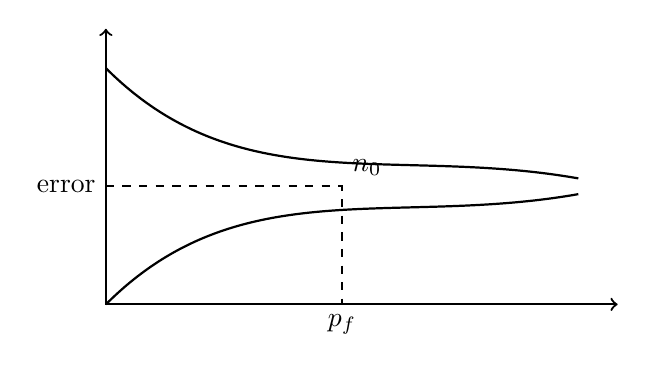
\begin{tikzpicture} [scale = 1] 

\draw[<->, thick] (0.0, 3.5) -- (0.0, 0.0) -- (6.5, 0.0);
\draw[dashed, thick] (0.0, 1.5) -- (3.0, 1.5) -- (3.0, 0.0);
\node[below, thick] at (3.0, 0.0){$p_{f}$};\node[left, thick] at (0.0, 1.5){error};\node[above right, thick] at (3.0, 1.5){$n_{0}$};
\draw[thick] (0.0, 0.0)to [out = 45, in = 190](6.0, 1.4);
\draw[thick] (0.0, 3.0)to [out = -45, in = 170](6.0, 1.6);
\end{tikzpicture} 
\end{figure}


\subsection{Analysis of Nearest Neighbor Classifier}
Given $\left\{\left(X_{i}, Y_{i}\right)\right\}_{i=1}^{n}$
\begin{align*}
&X_{i} \in \mathbb{R}^{d}
\end{align*}
predict $Y $ for new $X $

\begin{thm} \label{thm:ch} 
(Cover and Hart $60's) \mathbb{E}\left[R_{n} \left(X\right)\right] =$ expected error of NN classifier
\begin{align*}
\lim_{n\to \infty} \mathbb{E}\left[R_{n}\left(x\right)\right] &= \mathbb{E}\left[2 \eta\left(x\right) \left(1 - \eta\left(x\right)\right)\right] \leq  2 R^\star 
\end{align*}\end{thm}
as $n \to  \infty$, NN of $X $, say $x' \in \left\{x_{i}\right\}_{i=1}^{n}, x \approx x'$
\\* errs: $Y = 1, Y' = 0$ or $Y = 0, Y' = 1$
\begin{align*}
\eta\left(x\right)\left(1 - \eta\left(x'\right)\right) + \left(1 - \eta\left(x\right)\right) \eta\left(x'\right) &\approx 2 \eta\left(x\right) \left(1 - \eta\left(x\right)\right)
\end{align*}
\begin{align*}
z  :&= \displaystyle\min\left\{\eta\left(x\right), 1 - \eta\left(x\right)\right\}
\\ \eta\left(x\right)\left(1 - \eta\left(x\right)\right) &= z \left(1 - z\right)
\\ \mathbb{E}\left[\eta\left(x\right)\left(1 - \eta\left(x\right)\right)\right] &= \mathbb{E}\left[z \left(1 - z\right)\right] = \mathbb{E}\left[z - z^{2}\right]
\\ &= \mathbb{E}\left[z\right] - \underbrace{\mathbb{E}\left[z^{2}\right]}_{\geq  \mathbb{E}\left[z\right]^{2} \text{\;Jensen's Inequality\;}}
\\ &\leq  \mathbb{E}\left[z\right] - \mathbb{E}\left[z\right]^{2}
\\ &= \mathbb{E}\left[z\right] \left(1 - \mathbb{E}\left[z\right]\right)
\\ &\leq  \mathbb{E}\left[z\right]
\end{align*}





\section{Lecture $3$} 


\subsection{Matrices}
\begin{align*}
&u_{1}, u_{2}, u_{3}
\\ \left\|u_{1}\right\| &= \left\|u_{2}\right\| = 1
\\ u_{i}^{T} u_{j} &= 0, i \neq  j 
\\ U  &= \left[u_{1} u_{2} ... u_{m}\right], u_{i} \in \mathbb{R}^{n}
\end{align*}
Orthogonal matrix
\begin{align*}
U^{T} U &= I_{m}
\\ U^{T} U &= \begin{bmatrix} u_{1}^{T} \\ ... \\ u_{m}^{T} \end{bmatrix} \begin{bmatrix} u_{1} & ... & u_{m} \end{bmatrix} \begin{bmatrix} u_{1}^{T} u_{1} & ... & u_{1}^{T} u_{m} \\ ... & ... & ... \\ u_{m}^{T} u_{1} & ... & u_{m}^{T} u_{m} \end{bmatrix}
\\ &= \begin{bmatrix} 1 & ... & 0 \\ ... & ... & ... \\ 0 & ... & 1 \end{bmatrix}
\end{align*}

\begin{align*}
\mathbb{R}^{n} &= S \oplus S^{\bot}
\\ &  \left\{\hat{u}_{1}, \hat{u}_{2}\right\} \in S, \left\{\hat{u}_{3}\right\} \in S^{\bot}
\end{align*}
\begin{align*}
y  &= A x, y \in \mathbb{R}^{m}, A \in M_{m \times n}, x \in \mathbb{R}^{n}
\end{align*}
\begin{align*}
\begin{bmatrix} y_{r} \\ y_{m} \end{bmatrix} &= \begin{bmatrix} \sigma_{i} & 0 \\ 0 & 0 \end{bmatrix} \begin{bmatrix} x_{r} \\ x_{m} \end{bmatrix}
\\ y_{r} &= \begin{bmatrix} y_{1} \\ ... \\ y_{r} \end{bmatrix}
\\ y_{m} &= \begin{bmatrix} y_{r+1} \\ ... \\ y_{m} \end{bmatrix}, \text{\;always zero\;}
\\ \sigma_{i} &= \begin{bmatrix} \sigma_{1} & ... & 0 \\ ... & ... & ... \\ 0 & ... & \sigma_{r} \end{bmatrix}
\\ x_{r} &= \begin{bmatrix} x_{1} \\ ... \\ x_{r} \end{bmatrix}
\\ x_{m} &= \begin{bmatrix} x_{r+1} \\ ... \\ x_{n} \end{bmatrix}, \text{\;don't matter\;}
\end{align*}
\begin{align*}
\mathbb{R}^{m} &= \underbrace{N\left(A\right)}_{n - r} \oplus \underbrace{N\left(A\right)^{\bot}}_{r }
\end{align*}
where $N\left(A\right) $ is the nullspace
\begin{align*}
\mathbb{R}^{m} &= \underbrace{R\left(A\right)}_{r} \oplus \underbrace{R\left(A\right)^{\bot}}_{n - r}
\end{align*}


\subsection{SVD}
\begin{align*}
\underbrace{A}_{m \times n} &= \underbrace{U}_{m \times m} \underbrace{\Sigma}_{m \times n} \underbrace{V^{T}}_{n \times n}
\\ U^{T}  U &= I 
\end{align*}
if $U $ square, $U^{T} = U^{-1}$
\begin{align*}
\left\| U x \right\|^{2} &= \left(U x\right)^{T} \left(U x\right) = x^{T} U^{T} U x = x^{T} x = \left\|x \right\|
\\ \left(U  x\right)^{T} \left(U y\right) &= x^{T} U^{T} U y = x^{T} y 
\end{align*}
\begin{align*}
y  &= A x = U \Sigma V^{T} x, V^{T} x = \begin{bmatrix} v_{1}^{T} x \\ ... \\ v_{n}^{T} x \end{bmatrix}
\\ V  V^{T} x &= \left(v_{1} v_{1}^{T} + v_{2} v_{2}^{T} + v_{3} v_{3}^{T}\right) x = \left(v_{1}^{T} x\right) v_{1} + \left(v_{2}^{T} x\right) v_{2} + \left(v_{3}^{T} x\right) v_{3}
\\ x  &= v_{i}
\\ y  &= \sigma_{i} u_{i}
\\ r  &= \text{\;rank\;}\left(A\right)
\end{align*}
\begin{align*}
R\left(A\right)  &= \left\{u_{1}, ..., u_{r}\right\}
\\ R\left(A\right) ^{\bot} &= \left\{u_{r+1}, ..., u_{m}\right\}
\\ N\left(A\right)  &= \left\{v_{r+1}, ..., r_{n}\right\}
\\ N\left(A\right) ^{\bot} &= \left\{v_{1}, ..., v_{r}\right\}
\end{align*}


\subsection{Matrix Identities}
\begin{align*}
\begin{bmatrix} I & 0 \\ X & I \end{bmatrix} ^{-1} &= \begin{bmatrix} I & 0 \\ -X & I \end{bmatrix}
\\ \begin{bmatrix} I & 0 \\ X & I \end{bmatrix} \begin{bmatrix} I & 0 \\ -X & I \end{bmatrix} &= \begin{bmatrix} I & 0 \\ 0 & I \end{bmatrix}
\end{align*}
\begin{align*}
&\begin{bmatrix} X \\ Y \end{bmatrix} \sim  \left(0, \begin{bmatrix} \Sigma_{x} & \Sigma_{x,y} \\ \Sigma_{y,x} & \Sigma_{y} \end{bmatrix}\right)
\\ &X  | Y \sim  \left(..., \Sigma_{x} - \Sigma_{x,y} \Sigma_{y^{-1}} \Sigma_{y,x}\right)
\end{align*}
\begin{align*}
A  x_{1} + B x_{2} &= y_{1}
\\ C  x_{1} + D x_{2} &= y_{2}
\\ x_{1} &= A^{-1}\left(y_{1} - B x_{2}\right)
\\ C  A^{-1} y_{1} - C A^{-1} B x_{2} + D x_{2} &= y_{2}
\\ \left(D  - C A^{-1} B\right) x_{2} &= \left(y_{2} - C A^{-1} y_{1}\right)
\end{align*}
Matrix Iversion Lemma
\begin{align*}
\left(A  - B D^{-1} C\right)^{-1} &= A^{-1} + A^{-1} B \left(D - C A^{-1} B\right)^{-1} C A^{-1}
\end{align*}
Other Identities:
\begin{align*}
A  \left(I + A\right)^{-1} &= I - \left(I + A\right)^{-1}
\\ A  &= \left(I + A\right) - I 
\end{align*}


\subsection{Vector derivatives}
\begin{align*}
f\left(x\right)  &= 0, f:\mathbb{R}^{n} \to  \mathbb{R}
\\ \dfrac{\partial f}{\partial x_{1}} &= 0 \text{\;and\;} \dfrac{\partial f}{\partial x_{2}} = 0
\\ \dfrac{d f}{d x} &= \text{\;gradient\;} = \nabla  f 
\\ &f  : \mathbb{R}^{n} \to  \mathbb{R}^{m}
\\ \dfrac{d f}{d x} \in \mathbb{R}^{m \times n} &= \text{\;Jacobian\;}
\\ c^{T} x &= c_{1} x_{1} + ... + c_{n} x_{n}
\\ \dfrac{d c^{T} x}{d x} &= \begin{bmatrix} c_{1} \\ ... \\ c_{n} \end{bmatrix} = c 
\\ \dfrac{d x^{T} Q x}{d x} &= \left(Q + Q^{T}\right) x 
\end{align*}
\begin{align*}
&\displaystyle\min_{x} \left\| A x - b \right\|^{2}
\\ \left(A  x - b\right)^{T} \left(A x - b\right) &= x^{T} \left(A^{T} A\right) x - 2 b^{T} A x + b^{T} b 
\\ \dfrac{d \text{\;above\;}}{d x} &= 2 A^{T} A x - 2 A^{T} b = 0
\\ A^{T}  A x - A^{T} b &= 0
\\ x_{opt} &= \left(A^{T} A\right)^{-1} A^{T} b 
\end{align*}





\section{Lecture $4$} 


\subsection{Bayes Classifier}

\begin{align*}
&\left(X , Y\right) \sim  \mathbb{P}_{X Y}
\\ \eta\left(x\right) :&= \mathbb{P}\left\{Y = 1 | X = x \right\}
\end{align*}
\[ f^\star \left(x\right) =\left\{ \begin{array}{ll}
1& \text{\;if\;} \eta\left(x\right) \geq  \dfrac{1}{2} \\
0& \text{\;otherwise\;} \\
\end{array}\right. \]
\begin{align*}
\mathbb{P}\left\{f^\star \left(X\right) \neq  Y\right\} &= \mathbb{E}_{x\left[\displaystyle\min\left(\eta\left(X\right), 1 - \eta\left(X\right)\right)\right]}
\\ &\left\{\left(X_{i}, Y_{i}\right)\right\}_{i=1}^{n} \stackrel{iid}{\sim} \mathbb{P}_{X Y}
\end{align*}


\subsection{Nearest Neighbor Classifier}
new unlabeled example $x, $
\begin{align*}
i_{1nn\left(x\right)} &= \arg\displaystyle\min_{i = 1 ... n} \left\|x - x_{i}\right\|
\\ \hat{y} &= y_{i_{1nn\left(x\right)}} \leftarrow f_{1nn} \left(x\right)
\end{align*}
\begin{thm} \label{thm:1nn} 
The following inequality holds,
\begin{align*}
\lim_{n \to  \infty} \mathbb{P}\left\{f_{1nn} \left(X\right) \neq  Y\right\} &\leq  \mathbb{E}\left[2 \eta\left(X\right) \left(1 - \eta\left(X\right)\right)\right] \leq  2 \mathbb{P}\left\{f^\star \left(X\right) \neq  Y \right\}
\end{align*}\end{thm}
\begin{thm} \label{thm:1kmm} 
Let $R_{k}^{\infty} = \lim_{n \to  \infty} \mathbb{P}\left\{f_{knn}\left(X\right) \neq  Y \right\}$
\begin{align*}
\mathbb{P}\left\{f^\star \left(X\right) \neq  Y\right\} &\leq  R_{k}^{\infty} \leq  R_{l}^{\infty} \text{\;for\;} l  < k 
\end{align*}\end{thm}


\subsection{KNN Classifier}
\begin{thm} \label{thm:knn} 
(Stone '$77$) Let $k  \to  \infty$ and $\dfrac{k}{n} \to  0$ as $n  \to  \infty$, then,
\begin{align*}
\lim_{n \to  \infty} \mathbb{P}\left\{f_{1nn} \left(X\right) \neq  Y\right\} &= \mathbb{P}\left\{f^\star \left(X\right) = Y \right\}
\end{align*}\end{thm}
\begin{align*}
&  n  \to  k = \sqrt{n}
\\ &  \mathbb{P}\left\{f_{1nn} \left(X\right) \neq  Y\right\} - \mathbb{P}\left\{f^\star \left(X\right) = Y \right\} \to  0 \text{\;as\;} n \to  \infty
\end{align*}


\subsection{Histogram Classifier}
\begin{align*}
&X_{i} \in \left[0, 1\right]^{d}, Y_{i} \in \left\{0, 1\right\}
\\ d  &= 2
\end{align*}
"bin", $\left\{B_{i}\right\}_{j=1}^{M}$ bins, $M  = m^{d}$

\begin{align*}
\hat{p}_{j} &= \dfrac{\displaystyle\sum_{i=1}^{n} \mathbbm{1}_{x_{i} \in B_{j}, y_{i} = 1}}{\displaystyle\sum_{i=1}^{n} \mathbbm{1}_{x_{i} \in B_{j}}}, j = 1, ... M 
\end{align*}
if $x \in B_{j}$ and $\hat{p}_{j} \geq  \dfrac{1}{2}$ then label $1$, otherwise $0$.
\begin{align*}
\hat{\eta}_{n}\left(x\right) &= \displaystyle\sum_{j=1}^{M} \hat{p}_{j} \mathbbm{1}_{x \in B_{j}}
\end{align*}
\[ \hat{f}_{n}\left(x\right) =\left\{ \begin{array}{ll}
1& \text{\;if\;} \hat{\eta}_{n}\left(x\right) \geq  \dfrac{1}{2} \\
0& \text{\;otherwise\;} \\
\end{array}\right. \]
\begin{thm} \label{thm:hist} 
Let $M  \to  \infty$ and $\dfrac{n}{M} \to  \infty$ as $n \to  \infty$. Then,
\begin{align*}
&\mathbb{P}\left\{\hat{f}_{n}\left(X\right) \neq  Y\right\} \to  \mathbb{P}\left\{f^\star \left(X\right) \neq  Y \right\}
\end{align*}\end{thm}
\begin{lem} \label{lem:histl} 
,
\begin{align*}
\mathbb{P}\left\{\hat{f}_{n}\left(X\right) \neq  Y\right\} - \mathbb{P}\left\{f^\star \left(X\right) \neq  Y\right\} &\leq  2 \mathbb{E}\left[| \hat{\eta}_{n}\left(x\right) - \eta\left(x\right) |\right]
\end{align*}\end{lem}
\begin{align*}
p_{j} &= \mathbb{P}\left\{Y = 1 | X \in B_{j}\right\}
\\ p_{j} &= \dfrac{\displaystyle\int_{B_{j}} \eta\left(x\right) p_{x}\left(x\right) dx}{\displaystyle\int_{B_{j}} p_{x}\left(x\right) dx}
\end{align*}
\begin{align*}
\eta^{-x} &= \displaystyle\sum_{j}^{M} p_{j} \mathbbm{1}_{x \in B_{j}}
\end{align*}
\begin{align*}
\mathbb{E}\left[|\eta\left(x\right) - \hat{\eta}_{n}\left(x\right) |\right] &\leq  \underbrace{\mathbb{E}\left[|\eta\left(x\right) - \eta^{-_{n\left(x\right)}} |\right]}_{\text{\;Bias\;}, \to  0 as  M \to  \infty} + \underbrace{\mathbb{E}\left[|\eta^{-x} - \hat{\eta}_{n}\left(x\right) |\right]}_{\text{\;Variance\;}}
\end{align*}





\section{Lecture $5$} 


\subsection{Bayes Classifier}
\begin{align*}
\eta\left(x\right) &= \mathbb{P}\left\{Y = 1 | X = x \right\}
\end{align*}
\[ f^\star \left(x\right) =\left\{ \begin{array}{ll}
1& \text{\;if\;} \eta\left(x\right) \geq  \dfrac{1}{2} \\
0& \text{\;otherwise\;} \\
\end{array}\right. \]
Ideal Histogram Classifier

\begin{align*}
X  \in \left[0, 1\right]^{d}, Y &= \left\{0, 1\right\}
\\ M  &= m^{d} \text{\;"Bins"\;}, \left\{B_{j}\right\}_{j=1}^{\infty}
\\ p_{j} &= \dfrac{\mathbb{E}\left[\mathbbm{1}_{X \in B_{j}, Y = 1}\right]}{\mathbb{E}\left[\mathbbm{1}_{X \in B_{j}}\right]}
\\ &= \dfrac{\displaystyle\int_{B_{j}} \eta\left(x\right) p\left(x\right) d x}{\displaystyle\int_{B_{j}} p\left(x\right) d x}
\\ \bar{\eta}\left(x\right) &= \displaystyle\sum_{j=1}^{M} p_{j} \mathbbm{1}_{x \in B_{j}}
\end{align*}
\[ \bar{f}\left(x\right) =\left\{ \begin{array}{ll}
1& \text{\;if\;} \bar{\eta}\left(x\right) \geq  \dfrac{1}{2} \\
0& \text{\;otherwise\;} \\
\end{array}\right. \]
Empiritcal Histogram Classifier
\begin{align*}
\hat{p}_{j} &= \dfrac{\displaystyle\sum_{i=1}^{n} \mathbbm{1}_{x_{i} \in B_{j}, y_{i} = 1}}{\displaystyle\sum_{i=1}^{n} \mathbbm{1}_{x_{i} \in B_{j}}}
\\ &  \left\{\left(x_{i}, y_{j}\right)\right\} \stackrel{iid}{\sim} P_{x y}
\\ \hat{\eta}\left(x\right) &= \displaystyle\sum_{j=1}^{M} \hat{p}_{j} \mathbbm{1}_{x \in B_{j}}
\end{align*}
\[ \hat{f}\left(x\right) =\left\{ \begin{array}{ll}
1& \text{\;if\;} \hat{\eta}\left(x\right) \geq  \dfrac{1}{2} \\
0& \text{\;otherwise\;} \\
\end{array}\right. \]
A1 $p\left(x\right)  \geq  c > 0 \;\forall\; x $
\\* A2 $\eta$ is uniformly continuous
\begin{align*}
p\left(x\right)  &\geq  c > 0 \text{\;and\;} \dfrac{n}{M} \to  \infty \Rightarrow  N\left(x\right) \to ^{as} \infty
\end{align*}
\begin{thm} \label{thm:ehc} 
If $M  \to  \infty, \dfrac{n}{M} \to  \infty$ as $n  \to  \infty$
\begin{align*}
&\underbrace{\mathbb{P}\left\{\hat{f}\left(X\right) \neq  Y\right\}}_{\mathbb{E}\left[\mathbbm{1}_{\hat{f}\left(X\right) \neq  Y}\right]} \to  \underbrace{\mathbb{P}\left\{f^\star \left(X\right) \neq  Y \right\}}_{\mathbb{E}\left[\mathbbm{1}_{f^\star \left(X\right) \neq  Y}\right]}
\end{align*}\end{thm}
\begin{proof} \label{proof:ehc} 
$\mathbb{P}\left\{\hat{f}\left(X\right) \neq  Y\right\} - \mathbb{P}\left\{f^\star \left(X\right) \neq  Y\right\} \leq  2 \mathbb{E}\left[|\eta\left(X\right) - \hat{\eta}\left(X\right)|\right]$
\begin{align*}
\mathbb{E}\left[| \eta\left(X\right) - \hat{\eta}\left(X\right) |\right] &= \mathbb{E}\left[|\eta\left(X\right) - \bar{\eta}\left(X\right) + \bar{\eta}\left(X\right) - \hat{\eta}\left(X\right)|\right]
\\ &\leq  \underbrace{\mathbb{E}\left[|\eta\left(X\right) - \bar{\eta}\left(X\right)|\right]}_{\text{\;deterministic error\;}} + \underbrace{\mathbb{E}\left[| \bar{\eta}\left(X\right) - \hat{\eta}\left(X\right) |\right]}_{\text{\;stochastic error\;} \to  0, as n \to  \infty}
\end{align*}
where,
\begin{align*}
\mathbb{E}\left[|\eta\left(X\right) - \bar{\eta}\left(X\right)|\right] &= \displaystyle\int |\eta\left(x\right) - \bar{\eta}\left(x\right)| p\left(X\right) dx
\\ &= \displaystyle\sum_{j=1}^{M} \displaystyle\int_{B_{j}} \underbrace{|\eta\left(x\right) - \bar{\eta}\left(x\right)|}_{\leq  \varepsilon_{m} \to  0} p\left(x\right) dx
\\ &\leq  \varepsilon_{m}
\end{align*}
and,
\begin{align*}
\mathbb{E}\left[\bar{|\eta}\left(X\right) - \hat{\eta}\left(X\right)|\right] &= \mathbb{E}\left[\mathbb{E}\left[| \bar{\eta}\left(x\right) - \dfrac{K\left(x\right)}{N\left(x\right)} | | X = x \right]\right]
\end{align*}
where,
\\* $x $ let $B\left(x\right) $ be its bin
\begin{align*}
K\left(x\right)  &= \displaystyle\sum_{i=1}^{n} \mathbbm{1}_{x_{i} \in B\left(x\right), y_{i} = 1}
\\ N\left(x\right)  &= \displaystyle\sum_{i=1}^{n} \mathbbm{1}_{x_{i} \in B\left(x\right)}
\end{align*}
$K\left(x\right)  | N\left(x\right) = n_{x} \sim $ Binomial$\left(n_{x}, \bar{\eta}\left(x\right)\right)$
\begin{align*}
\mathbb{E}\left[K\left(x\right) | N\left(x\right) = n_{x}\right] &= n_{x} \bar{\eta}\left(x\right)
\\ \mathbb{E}\left[\dfrac{K\left(x\right)}{N\left(x\right)} | N\left(x\right) = n_{x}\right] &= \dfrac{n_{x} \bar{\eta}\left(x\right)}{n_{x}} = \bar{\eta}\left(x\right)
\\ \mathbb{E}\left[\left(\bar{\eta}\left(x\right) - \dfrac{K\left(x\right)}{N\left(x\right)}\right)^{2} | N\left(x\right) = n_{x}\right] &= \mathbb{E}\left[\dfrac{1}{\left(n_{x}\right)^{2}} \left(n_{x} \bar{\eta}\left(x\right) - K\left(x\right)\right)^{2} | N\left(x\right) = n_{x}\right]
\\ &= \dfrac{1}{\left(n_{x}\right)^{2}} \mathbb{E}\left[\left(n_{x} \bar{\eta}\left(x\right) - K\left(x\right)\right)^{2} | X = x \right]
\\ &= \dfrac{1}{\left(n_{x}\right)^{2}} \left(n_{x} \bar{\eta}\left(x\right) \left(1 - \bar{\eta}\left(x\right)\right)\right)
\\ &= \dfrac{\bar{\eta}\left(x\right) \left(1 - \bar{\eta}\left(x\right)\right)}{n_{x}}
\end{align*}
Recall, $\mathbb{E}\left[Z^{2}\right] \geq  \left(\mathbb{E}\left[Z\right]\right)^{2}$ Jensen's
\begin{align*}
\mathbb{E}\left[| \bar{\eta}\left(X\right) - \hat{\eta}\left(X\right) | | X = x\right] &\leq  \sqrt{\dfrac{\bar{\eta}\left(x\right) \left(1 - \bar{\eta}\left(x\right)\right)}{n_{x}}}
\end{align*}\end{proof}
\begin{align*}
N\left(x\right)  &\propto \dfrac{n}{M}
\\ \mathbb{E}\left[\bar{|\eta}\left(X\right) - \hat{\eta}\left(X\right)|\right] &= O\left(\sqrt{\dfrac{M}{n}}\right)
\end{align*}
A3: $\eta$ is $1$-Lipschitz
\begin{align*}
| \eta\left(x\right) - \eta\left(x'\right) | &\leq  \| x - x' \| \;\forall\; x, x' \in \left[0, 1\right]^{d}
\end{align*}
if $x , x' \in B_{j}, \| x - x' \| \leq  \dfrac{\sqrt{d}}{m} =: \varepsilon_{m}$

\begin{align*}
\mathbb{P}\left\{\hat{f}\left(X\right) \neq  Y\right\} - \mathbb{P}\left\{f^\star \left(X\right) \neq  Y\right\} &= O\left\{\displaystyle\max\left(\sqrt{\dfrac{m^{d}}{n}}, \dfrac{\sqrt{d}}{m}\right)\right\}
\\ &  \sqrt{\dfrac{m^{d}}{n}} = \dfrac{\sqrt{d}}{m}
\\ &\Rightarrow  m^{d+2} = d n 
\\ &\Rightarrow  m = \left(d n\right)^{\dfrac{1}{d+2}}
\\ \mathbb{P}\left\{\hat{f}\left(X\right) \neq  Y\right\} - \mathbb{P}\left\{f^\star \left(X\right) \neq  Y\right\} &= O\left( \dfrac{\sqrt{d}}{\left(d n\right)^{\dfrac{1}{d+2}}}\right)
\\ &= O\left(\dfrac{1}{n^{\dfrac{1}{d+2}}}\right)
\\ &= O\left(n^{- \dfrac{1}{d+2}}\right)
\end{align*}
Curse of dim



\subsection{Multivariate Normal Distribution}
\begin{align*}
&X  \in \mathbb{R}^{d}
\\ p\left(x\right)  &= \dfrac{1}{\sqrt{\left(2 \pi\right)^{d} | \Sigma |}} \exp\left(- \dfrac{1}{2} \left(x - \mu\right)^{T} \Sigma^{-1} \left(x - \mu\right)\right)
\\ \mu \in \mathbb{R}^{d}, \mathbb{E}\left[X\right] &= \mu, \Sigma = \mathbb{E}\left[\left(X - \mu\right)\left(X - \mu\right)^{T}\right] \in \mathbb{R}^{d \times d}
\\ \Sigma_{ij} &= \mathbb{E}\left[\left(X_{i} - \mu_{i}\right)\left(X_{j} - \mu_{j}\right)\right]
\end{align*}
Covariation of $X_{i}, X_{j}$
\begin{align*}
&X  \sim  N\left(\mu, \Sigma\right)
\end{align*}

If $x  \sim  N\left(\mu, \Sigma\right)$, then $A  x + b \sim  N\left(A \mu + b, A \Sigma A^{T}\right)$

Bivariate: $X  = \begin{bmatrix} x_{1} \\ x_{2} \end{bmatrix} , \mathbb{E}\left[X\right] = \begin{bmatrix} m_{1} \\ m_{2} \end{bmatrix} , \Sigma = \begin{bmatrix} 1 & 0 \\ 0 & 1 \end{bmatrix}$

\begin{align*}
\Sigma &= \begin{bmatrix} 1 & - \dfrac{1}{2} \\ - \dfrac{1}{2} & 1 \end{bmatrix}
\end{align*}
\begin{align*}
\Sigma &= \begin{bmatrix} 1 & 0 \\ 0 & 2 \end{bmatrix}
\end{align*}
MVN Classifier
\\* Suppose $X  | Y = l \sim  \underbrace{N\left(\mu_{l}, \Sigma_{l}\right)}_{\text{\;class-conditional distribution of\;} x }, l = 0, 1, ..., k - 1$
\begin{align*}
&  \mathbb{P}\left\{Y = l\right\} = \dfrac{1}{K}
\\ &  \mathbb{P}\left\{X | Y = l\right\} \mathbb{P}\left\{Y = l\right\}
\end{align*}
Bayes Classifier
\begin{align*}
f^\star \left(x\right) &= \arg\displaystyle\max_{l} p\left(x | y = l\right) \mathbb{P}\left\{Y = l \right\}
\\ K  &= 2
\end{align*}
\[ f^\star \left(x\right) =\left\{ \begin{array}{ll}
1& \text{\;if\;} \underbrace{\log\left(\dfrac{p\left(x | y = 1\right)}{p\left(x | y = 0\right)}\right)}_{\log \text{\;likelihood ratio\;}} \geq  0 \\
0& \text{\;otherwise\;} \\
\end{array}\right. \]
Log LR
\begin{align*}
&  \log\left(\dfrac{\dfrac{1}{\sqrt{\left(2 \pi\right)^{d} | \Sigma_{1} |}} \exp\left(- \dfrac{1}{2} \left(x - \mu_{1}\right)^{T} \Sigma_{1}^{-1} \left(x - \mu_{1}\right)\right)}{\dfrac{1}{\sqrt{\left(2 \pi\right)^{d} | \Sigma_{0} |}} \exp\left(- \dfrac{1}{2} \left(x - \mu_{0}\right)^{T} \Sigma_{0}^{-1} \left(x - \mu_{0}\right)\right)}\right)
\\ &= \underbrace{- \dfrac{1}{2} \left(x - \mu_{1}\right)^{T} \Sigma_{1}^{-1} \left(x - \mu_{1}\right) + \dfrac{1}{2} \left(x - \mu_{0}\right)^{T} \Sigma_{0}^{-1} \left(x - \mu_{0}\right)}_{\text{\;quadratic in\;} x } + \text{\;const\;}
\end{align*}

If $\Sigma_{0} = \Sigma_{1} = \Sigma$,
\[ \hat{y}\left(x\right) =\left\{ \begin{array}{ll}
1& \text{\;if\;} \underbrace{2\left(\mu_{1} - \mu_{0}\right)^{T} \Sigma^{-1}}_{w} x \geq  \underbrace{\mu_{0}^{T} \Sigma \mu_{0} - \mu_{1}^{T} \Sigma \mu_{1}}_{t } \\
0& \text{\;otherwise\;} \\
\end{array}\right. \]
Linear classifier $w^{T} x > t $

\begin{align*}
&\left\{x_{i}, y_{i}\right\}_{i=1}^{n}
\\ \hat{\mu}_{1} &= \dfrac{1}{n_{1}} \displaystyle\sum_{i \in Y_{i} = 1} x_{i}, n_{1} = \text{\;number of\;} Y_{i} = 1
\\ \hat{\Sigma}_{1} &= \dfrac{1}{n_{1}} \displaystyle\sum_{i \in Y_{i} = 1} \left(x_{i} - \hat{\mu}_{1}\right) \left(x_{i} - \hat{\mu}_{1}\right)^{T}
\end{align*}





\section{Lecture $6$} 


\subsection{Generative Models}

$Y  = 0$ or $Y  = 1$
\begin{align*}
\mathbb{P}\left\{Y = 0\right\} &= 1 - \mathbb{P}\left\{Y = 1\right\}
\end{align*}
$\mathbb{P}\left\{X | Y = 0\right\}, P\left\{X | Y = 1\right\}$, Class-conditional distributions
\begin{align*}
X  | Y &= 0 \sim  N\left(\mu_{0}, \Sigma_{0}\right)
\\ X  | Y &= 1 \sim  N\left(\mu_{1}, \Sigma_{1}\right)
\end{align*}
Region $\hat{y} = 0$ is $R_{0}$, region $\hat{y} = 1$ is $R_{1}, x  \in X $
\begin{align*}
X  &= R_{0} \cup R_{1}
\\ \left(X , Y\right) \sim  \mathbb{P}_{x,y} &= \mathbb{P}\left\{X = x, Y = y\right\} = \mathbb{P}\left\{X | Y = y\right\} \mathbb{P}\left\{Y = y\right\}
\\ \text{\;Total Err\;} &= c_{10} \mathbb{P}\left\{Y = 0, \hat{Y} = 1\right\} + c_{01} \mathbb{P}\left\{Y = 1, \hat{Y} = 0\right\}, c_{10}, c_{01} > 0
\\ &= c_{10} \displaystyle\int_{R_{1}} \underbrace{p\left(x | y = 0\right) p\left(y = 0\right)}_{\geq  0} dx + c_{01} \displaystyle\int_{R_{0}} \underbrace{p\left(x | y = 1\right) p\left(y = 1\right)}_{\geq  0} dx
\end{align*}
Aside,
\\* $X $ with density $p\left(x\right) , A $ sub $X , \mathbb{P}\left\{X \in A\right\} = \displaystyle\int_{A} p\left(x\right) dx$

If $p\left(x | y = 0\right)  p\left(y = 0\right) > p\left(x | y = 1\right) p\left(y = 1\right)$
\\* Then put $x $ in $R_{0}$
\\* Conversely if $<$, then $x $ in $R_{1}$
\begin{align*}
&  \dfrac{p\left(x | y = 1\right) p\left(y = 1\right)}{p\left(x | y = 0\right) p\left(y = 0\right)} \gtreqless^{\hat{y} = 1}_{\hat{y} = 0} 1
\\ \text{\;LR\;} &= \dfrac{p\left(x | y = 1\right)}{p\left(x | y = 0\right)} \gtreqless^{\hat{y} = 1}_{\hat{y} = 0} \dfrac{c_{10} p\left(y = 0\right)}{c_{01} p\left(y = 1\right)}
\\ \text{\;LRT\;} &= \dfrac{p\left(x | y = 1\right)}{p\left(x | y = 0\right)} \gtreqless^{\hat{y} = 1}_{\hat{y} = 0} t 
\end{align*}


\subsection{Constrain one type of error}

\begin{align*}
\displaystyle\min \mathbb{P}\left\{\hat{y} = 0, Y = 1\right\} \text{\;such that\;} \mathbb{P}\left\{\hat{y} = 1, Y = 0\right\} &\leq  \alpha < 1
\end{align*}
Neyman-Pearson decision
\\* Solution:
\begin{align*}
&\dfrac{p\left(x | y = 1\right)}{p\left(x | y = 0\right)} \gtreqless^{\hat{y} = 1}_{\hat{y} = 0} t_{\alpha}
\end{align*}
Example
\\* If $X  | Y = j \sim  N\left(\mu_{j}, \Sigma_{j}\right)$
\begin{align*}
p\left(x | y = j\right)  &= \dfrac{1}{\sqrt{\left(2 \pi\right)^{d} | \Sigma_{j} |}} e^{- \dfrac{1}{2} \left(x - \mu_{j}\right)^{T} \Sigma^{-1}_{j} \left(x - \mu_{j}\right)}
\\ \log\left(p\left(x | y = j\right)\right) &= - \dfrac{1}{2} \underbrace{\left(x - \mu_{j}\right)^{T} \Sigma^{-1}_{j} \left(x - \mu_{j}\right)}_{\text{\;Mahanalobis distance\;}} + \text{\;constant\;}
\end{align*}
Special case:
\begin{align*}
\Sigma_{0} &= \Sigma_{1} = \Sigma
\end{align*}
Linear classifier

$\left\{\left(X_{i}, Y_{i}\right)\right\} \stackrel{iid}{\sim} \mathbb{P}_{X,Y}$ MVN cross conditionals
\begin{align*}
j  &= 0, 1
\\ &\Rightarrow  \hat{\mu}_{j} = \dfrac{1}{\#\left\{i : y_{i} = j\right\}} \displaystyle\sum_{i : y_{i} = j} x_{i}
\\ \hat{\Sigma}_{j} &= \dfrac{1}{\#\left\{i : y_{i} = j\right\}} \displaystyle\sum_{i : y_{i} = j} \left(x_{i} - \hat{\mu}_{j}\right)\left(x_{i} - \hat{\mu}_{j}\right)^{T}
\\ \mu_{j} &= \mathbb{E}\left[X | Y = j\right]
\\ \Sigma_{j} &= \mathbb{E}\left[\left(X - \mu_{j}\right)\left(X - \mu_{j}\right)^{T} | Y = j\right]
\end{align*}
Is there a natural notion of "distance" for general class-conditional distributions?
\begin{align*}
p_{0}\left(x\right) &= \mathbb{P}\left\{X | Y = 0\right\}
\\ p_{1}\left(x\right) &= \mathbb{P}\left\{X | Y = 1\right\}
\\ \log \text{\;LR\;} &= \log \dfrac{P_{1}\left(x\right)}{P_{0}\left(x\right)} = \Lambda\left(x\right) \gtreqless^{\hat{y} = 1}_{\hat{y} = 0} 0
\end{align*}
if $X  \sim  q  \left(q \right.$ may be $P_{0}$ or $P_{1}$ or even something else)
\\* What do we expect $\log \text{\;LR\;}$ to be?
\begin{align*}
\mathbb{E}_{q\left[\Lambda\left(X\right)\right]} &= \displaystyle\int q\left(x\right) \log\left(\dfrac{p_{1}\left(x\right)}{p_{0}\left(x\right)}\right) dx
\\ &= \displaystyle\int q\left(x\right) \log\left(\dfrac{p_{1}\left(x\right)}{p_{0}\left(x\right)} \cdot  \dfrac{q\left(x\right)}{q\left(x\right)}\right) dx
\\ &= \displaystyle\int q\left(x\right) \log\left(\dfrac{q\left(x\right)}{p_{0}\left(x\right)}\right) dx - \displaystyle\int q\left(x\right) \log\left(\dfrac{q\left(x\right)}{p_{1}\left(x\right)}\right) dx
\\ &= D\left(q \| p_{0}\right) - D\left(q \| p_{1}\right)
\end{align*}
KLD of $p_{i}$ from $q $, Kullback-Leibler divergence
\begin{align*}
&D\left(q \| p_{0}\right)  \gtreqless^{\hat{y} = 1}_{\hat{y} = 0} D\left(q \| p_{1}\right) 
\end{align*}
KL for MVN
\begin{align*}
D\left(N\left(\mu_{0}, \Sigma_{0}\right) \| N\left(\mu_{1}, \Sigma_{1}\right)\right)  &= \dfrac{1}{2} \left(tr\left(\Sigma^{-1}_{1} \Sigma_{0}\right)  + \left(\mu_{1} - \mu_{0}\right)^{T} \Sigma^{-1}_{1} \left(\mu_{1} - \mu_{0}\right) - d + \log\left(\dfrac{| \Sigma_{1} |}{| \Sigma_{0} |}\right)\right)
\end{align*}
\begin{align*}
D\left(q \| p\right)  &\geq  0
\end{align*}





\section{Lecture $7$} 


\subsection{Optimal Classification}
\begin{align*}
&\left(X , Y\right) \sim  \mathbb{P}_{X,Y}
\end{align*}
$p\left(x, y\right) $ be joint prob density or mass function
\begin{align*}
p\left(y | x\right)  &= \dfrac{p\left(x, y\right)}{p\left(x\right)}
\end{align*}
explicit notation
\begin{align*}
p\left(y | x\right)  &= \mathbb{P}\left\{Y = y | X = x\right\}
\\ \eta\left(x\right) &= \mathbb{P}\left\{Y = 1 | X = x\right\}
\\ 1 - \eta\left(x\right) &= \mathbb{P}\left\{Y = 0 | X = x\right\}
\end{align*}
$\displaystyle\min$ prob of error classifier
\[ f^\star \left(x\right) =\left\{ \begin{array}{ll}
0& \text{\;if\;} \eta\left(x\right) \geq  \dfrac{1}{2} \\
0& \text{\;otherwise\;} \\
\end{array}\right. \]
\begin{align*}
\eta\left(x\right) &\geq  \dfrac{1}{2} \Leftrightarrow  \dfrac{\eta\left(x\right)}{1 - \eta\left(x\right)} \geq  1
\\ \dfrac{\eta\left(x\right)}{1 - \eta\left(x\right)} &= \dfrac{\mathbb{P}\left\{Y = 1 | X = x\right\}}{\mathbb{P}\left\{Y = 0 | X = x\right\}} = \dfrac{p\left(y = 1 | x\right)}{p\left(y = 0 | x\right)}
\\ &= \dfrac{\dfrac{p\left(x, y = 1\right)}{p\left(x\right)}}{\dfrac{p\left(x, y = 0\right)}{p\left(x\right)}} = \dfrac{p\left(x, y = 1\right)}{p\left(x, y = 0\right)}
\\ &= \dfrac{p\left(x | y = 1\right) p\left(y = 1\right)}{p\left(x | y = 0\right) p\left(y = 0\right)} = \text{\;LR\;}
\end{align*}
\begin{align*}
p\left(x, y\right)  &= p\left(y | x\right) p\left(x\right) 
\\ &= p\left(x | y\right) p\left(y\right) 
\end{align*}
class-conditional distribution

\begin{align*}
p_{0}\left(x\right) &= p\left(x | y = 0\right)
\\ p_{1}\left(x\right) &= p\left(x | y = 1\right)
\\ \Lambda\left(x\right) &= \log\left(\dfrac{p_{1}\left(x\right)}{p_{0}\left(x\right)}\right)
\\ &\Lambda \gtreqless^{\hat{y} = 1}_{\hat{y} = 0} 0
\end{align*}
$X  \sim  q $ prob dist ("test")
\\* $\Lambda\left(X\right)$ is a real-valued random variable
\begin{align*}
\Lambda\left(X\right) &= \underbrace{\mathbb{E}\left[\Lambda\left(X\right)\right]}_{\text{\;deterministic, a number\;}} + \underbrace{\left(\Lambda\left(X\right) - \mathbb{E}\left[\Lambda\left(X\right)\right]\right)}_{\text{\;zero-mean random variable\;}}
\\ \mathbb{E}\left[\Lambda\left(X\right)\right] &= \displaystyle\int \Lambda\left(x\right) q\left(x\right) dx
\\ &= \displaystyle\int q\left(x\right) \log\left(\dfrac{p_{1}\left(x\right)}{p_{0}\left(x\right)} \cdot  \dfrac{q\left(x\right)}{q\left(x\right)}\right) dx
\\ &= \underbrace{\displaystyle\int q\left(x\right) \log\left(\dfrac{q\left(x\right)}{p_{0}\left(x\right)}\right) dx}_{D\left(q \| p_{0}\right)} - \underbrace{\displaystyle\int q\left(x\right) \log\left(\dfrac{q\left(x\right)}{p_{1}\left(x\right)}\right) dx}_{D\left(q \| p_{1}\right)}
\end{align*}
Kullback-Leibler (KL) divergences
\begin{lem} \label{lem:kl} 
$D\left(q \| p\right)  \geq  0$ for any $q , p $ distributions, $D\left(q \| q\right)  = 0$.
\end{lem}
\begin{proof} \label{proof:kl} 
,
\begin{align*}
D\left(q \| p\right)  &= \displaystyle\int q\left(x\right) \log\left(\dfrac{q\left(x\right)}{p\left(x\right)}\right) dx
\\ &= - \displaystyle\int q\left(x\right) \log\left(\dfrac{p\left(x\right)}{q\left(x\right)}\right) dx
\\ &= - \mathbb{E}_{q\left[\log\left(\dfrac{p\left(x\right)}{q\left(x\right)}\right)\right]}
\\ &\geq  - \log\left(\mathbb{E}\left[\dfrac{p\left(x\right)}{q\left(x\right)}\right]\right)
\\ &= - \log\left(\displaystyle\int q\left(x\right) \dfrac{p\left(x\right)}{q\left(x\right)} dx\right)
\\ &= - \log\left(1\right)
\\ &\geq  0
\end{align*}
Jensen's Inequality. If $f $ is convex, then $\mathbb{E}\left[f\left(Z\right)\right] \geq  f\left(\mathbb{E}\left[Z\right]\right)$
\end{proof}
\begin{align*}
&D\left(q \| p_{0}\right)  - D\left(q \| p_{1}\right)
\end{align*}
Case $1: q  = p_{1}$
\\* Case $2: q  = p_{0}$

\begin{eg} \label{eg:normlam} 
$X  | Y = 0 \sim  N\left(-\mu, 1\right), X  | Y = 1 \sim  N\left(\mu, 1\right)$
\begin{align*}
\Lambda\left(x\right) &= \log\left(\dfrac{\dfrac{1}{\sqrt{2 \pi}} e^{- \dfrac{\left(x - \mu\right)^{2}}{2}}}{\dfrac{1}{\sqrt{2 \pi}} e^{- \dfrac{\left(x + \mu\right)^{2}}{2}}}\right)
\\ &= - \dfrac{\left(x - \mu\right)^{2}}{2} +  \dfrac{\left(x + \mu\right)^{2}}{2}
\\ &= \dfrac{2 \mu x + 2 \mu x}{2}
\\ &= 2 \mu x \gtreqless^{\hat{y} = 1}_{\hat{y} = 0}
\\ \Lambda\left(x\right) &= 2 \mu x 
\end{align*}\end{eg}
\begin{align*}
&X  \sim  p_{1}
\\ \Lambda\left(x\right) &= 2 \mu X \sim  N\left(2 \mu^{2}, 4 \mu^{2}\right), \sigma = 2 \mu
\end{align*}
$\mu$ bigger is better
\\* MVN: $x  | y = j \sim  N\left(\mu_{j}, \Sigma\right), j = 0, 1$
\begin{align*}
D\left(p_{0} \| p_{1}\right)  &= D\left(p_{1} \| p_{0}\right) 
\\ &= \dfrac{1}{2} \left(\mu_{1} - \mu_{0}\right)^{T} \Sigma^{-1} \left(\mu_{1} - \mu_{0}\right)
\\ D\left(p_{1} \| p_{0}\right)  &= D\left(p_{0} \| p_{1}\right) 
\\ &= 2 \mu^{2}
\end{align*}





\section{Lecture $8$} 


\subsection{Bayes Classifier (minimum prob of err)}
\[ f^\star \left(x\right) =\left\{ \begin{array}{ll}
+1& \text{\;if\;} \mathbb{P}\left(y = 1 | X = x\right\} \geq  \dfrac{1}{2} \\
-1& \text{\;otherwise\;} \\
\end{array}\right. \]
or
\[ \left\{ \begin{array}{ll}
+1& \text{\;if\;} \log \left(\dfrac{p\left(x | y = 1\right)}{p\left(x | y = -1\right)}\right) \geq  \log \left(\dfrac{p\left(y = -1\right)}{p\left(y = +1\right)}\right) \\
-1& \text{\;otherwise\;} \\
\end{array}\right. \]


\subsection{Nearest Neighbor Classifier}
\begin{align*}
&  \left\{\left(X_{i}, Y_{i}\right)\right\} \stackrel{iid}{\sim} \mathbb{P}_{XY}
\\ f_{1nn}\left(x\right) &= y_{i_{x}}, i_{x} = \arg\displaystyle\min_{i} \left\|x - x_{i}\right\|
\\ \lim_{n\to \infty} \mathbb{P}\left\{f_{1nn}\left(X\right) \neq  Y\right\} &\leq  2 \mathbb{P}\left\{f^\star \left(X\right) \neq  Y\right\}
\end{align*}
\begin{eg} \label{eg:zerobayes} 
$x \in \left\{-1, 1\right\}^{d}, y \in \left\{-1, 1\right\}, y  = x_{1}$, and $x_{2}, ..., x_{d} \stackrel{iid}{\sim} \pm 1$ with probability $\dfrac{1}{2}$ .
\begin{align*}
\text{\;Bayes Error\;} &= 0
\\ n  &= 2, x  = \left(+1, +1, ..., +1\right)
\\ d  &= 2, x  = \left(1, 1\right)
\end{align*}
Possible cases for $\left(x_{1}, +1\right)$ and $\left(x_{2}, -1\right)$,

\begin{center} \begin{tabular}{|c|c|c|c|}
\hline
 $1$ &-$1$ &correct\\ \hline
-$1$ &$1$ &incorrect\\ \hline
$1$ &$1$ &correct\\ \hline
-$1$ &-$1$ &incorrect\\ \hline
$1$ &-$1$ &tie\\ \hline
-$1$ &$1$ &tie\\ \hline
$1$ &-$1$ &correct\\ \hline
-$1$ &-$1$ &incorrect\\ \hline
\end{tabular} \end{center}
\begin{align*}
\dfrac{1}{4} \cdot  \dfrac{1}{2} &= \dfrac{1}{8}
\\ &  \mathbb{P}\left\{f_{1nn}\left(X\right) \neq  Y\right\} \to  \dfrac{1}{2} \text{\;as\;} d  \to  \infty
\end{align*}\end{eg}


\subsection{Generative Model Plug-in Classifier}
\begin{align*}
p\left(y = +1\right)  &= p\left(y = -1\right)
\\ X  | Y &= +1 \sim  N\left(\theta, I\right)
\\ X  | Y &= -1 \sim  N\left(-\theta, I\right)
\end{align*}
Bayes Classifier
\begin{align*}
&- \dfrac{1}{2} \left\|x - \theta\right\|^{2} + \dfrac{1}{2} \left\|x + \theta\right\|^{2} - \dfrac{1}{2} \left\|x - \theta\right\|^{2} + \dfrac{1}{2} \left\|x + \theta\right\|^{2}
\end{align*}
\[ f^\star \left(x\right) =\left\{ \begin{array}{ll}
+1& \text{\;if\;} x^{T} \theta > 0 \\
-1& \text{\;if\;} x^{T} \theta < 0 \\
\end{array}\right. \]
Bayes Err Rate
\begin{align*}
\mathbb{P}\left\{f^\star \left(X\right) \neq  Y\right\} &= \dfrac{1}{2} \mathbb{P}\left\{x^{T} \theta > 0 | Y = -1\right\} + \dfrac{1}{2} \mathbb{P}\left\{x^{T} \theta < 0 | Y = +1\right\}
\\ \mathbb{P}\left\{x^{T} \theta > 0 | Y = -1\right\}, &  x^{T} \theta \sim  N\left(-\left\|\theta\right\|^{2}, \left\|\theta\right\|^{2}\right)
\\ \mathbb{P}\left\{Z > 0\right\} &= \mathbb{P}\left\{Z' > \left\|\theta\right\|^{2}\right\}, Z \sim  N\left(-\left\|\theta\right\|^{2}, \left\|\theta\right\|^{2}\right), Z' \sim  N\left(0, \left\|\theta\right\|^{2}\right)
\\ &\leq  \dfrac{\left\|\theta\right\|^{2}}{\left(\left\|\theta\right\|\right)^{4}}
\\ &= \dfrac{1}{\left\|\theta\right\|^{2}}
\end{align*}
Use Markov,
\begin{align*}
\mathbb{P}\left\{Z > t\right\} &\leq  \mathbb{P}\left\{Z^{2} > t^{2}\right\} \leq  \dfrac{\mathbb{E}\left[Z^{2}\right]}{t^{2}}
\end{align*}
Plug-in,
\begin{align*}
\hat{\theta} &= \dfrac{1}{n} \displaystyle\sum_{i=1}^{n} y_{i} x_{i}
\end{align*}
\[ \hat{f}\left(x\right) =\left\{ \begin{array}{ll}
+1& \text{\;if\;} x^{T} \hat{\theta} > 0 \\
-1& \text{\;if\;} x^{T} \hat{\theta} < 0 \\
\end{array}\right. \]
What is the distribution of $x^{T} \hat{\theta} | Y = -1$
\begin{align*}
X  &= -\theta + e_{1}, e_{1} \sim  N\left(0, I \right)
\\ \hat{\theta} &= \theta + e_{2}, e_{2} \sim  N\left(0, \dfrac{1}{n} I \right)
\end{align*}
Ignoring constant factors,
\begin{align*}
\mathbb{P}\left\{x^{T} \hat{\theta} > 0 | Y = -1\right\} &\leq  \dfrac{1}{\left\|\theta\right\|^{2}} + \dfrac{d^{2}}{n} \dfrac{1}{\left\|\theta\right\|^{4}}
\\ \dfrac{d^{2}}{n} \dfrac{1}{\left\|\theta\right\|^{4}} &\approx \dfrac{1}{\left\|\theta\right\|^{2}}
\\ n  &\approx \left(\dfrac{\left\|\theta\right\|}{d}\right)^{2}
\end{align*}


\subsection{Maximum Likelihood Estimation}
\begin{align*}
&x_{1}, ..., x_{n} \sim  q 
\\ &q  \in \left\{p_{\theta}\right\}_{\theta \in \Theta}
\end{align*}
\begin{eg} \label{eg:normalmle} 
$x_{1}, ..., x_{n} \stackrel{iid}{\sim} N\left(\theta, I \right)$ for some $\theta \in \mathbb{R}^{d}$
\end{eg}
Two approaches
\begin{enumerate}
\item Method of Moments
\begin{align*}
\mu_{f} &= \displaystyle\int f\left(x\right) q\left(x\right) dx, \text{\;for any\;} f 
\\ \hat{\mu}_{f} &= \dfrac{1}{n} \displaystyle\sum_{i=1}^{n} f\left(x_{i}\right)
\\ \mu_{f}\left(\theta\right) &= \displaystyle\int f\left(x\right) p_{\theta}\left(x\right) dx
\end{align*}
find $\theta$ that minimizes,
\begin{align*}
&| \hat{\mu}_{f} - \mu_{f}\left(\theta\right) | \to  \hat{\theta}
\end{align*}
for one or more functions $f. $
\item MLE
\begin{align*}
\hat{\theta} &= \arg\displaystyle\max_{\theta} \displaystyle\prod_{i=1}^{n} p_{\theta}\left(x_{i}\right)
\\ &= \arg\displaystyle\min_{\theta} - \displaystyle\sum_{i=1}^{n} \log p_{\theta}\left(x_{i}\right)
\end{align*}

\end{enumerate}




\section{Lecture $9$} 


\subsection{Maximum Likehood}
\begin{align*}
&x_{1}, ..., x_{n} \stackrel{iid}{\sim} q 
\end{align*}
Models $\left\{P_{\theta}\right\}_{\theta \in \Theta}$
\begin{align*}
L\left(\theta\right)  &= \log \left(\displaystyle\prod_{i=1}^{n} P_{\theta}\left(x\right)\right)
\end{align*}
when viewed as function of $\theta$ is called the likehood of $\theta$.
\begin{align*}
\hat{\theta} &= \arg\displaystyle\max_{\theta} L\left(\theta\right)
\end{align*}
\begin{eg} \label{eg:normmle} 
$x  | \theta \sim  N\left(\theta, I\right), \theta \in \mathbb{R}^{d}$
\begin{align*}
\log p\left(x | \theta\right) &= \log \left(\dfrac{1}{\sqrt{2 \pi d}} \exp\left(- \dfrac{1}{2} \left(x_{1} - \theta\right)^{T}\left(x_{1} - \theta\right)\right)\right)
\\ &= - \dfrac{1}{2} \left(x_{1} - \theta\right)^{T} \left(x_{1} - \theta\right) + \text{\;const\;}
\\ &= - \dfrac{1}{2} \left(x_{1}^{T} x_{1} - 2 x_{1}^{T} \theta + \theta^{T} \theta\right)
\\ \hat{\theta} &= \arg\displaystyle\max_{\theta \in \mathbb{R}^{d}} - \displaystyle\sum_{i=1}^{n} \dfrac{1}{2} \left(x_{1} - \theta\right)^{T} \left(x_{1} - \theta\right)
\\ &\Rightarrow  \displaystyle\sum_{i=1}^{n} \left(x_{i} - \theta\right) = 0
\\ &\Rightarrow  \displaystyle\sum x_{i} = \displaystyle\sum \theta
\\ &\Rightarrow  \displaystyle\sum x_{i} = n \theta
\\ &\Rightarrow  \hat{\theta} = \dfrac{1}{n} \displaystyle\sum x_{i}
\end{align*}\end{eg}
\begin{eg} \label{eg:poissmle} 
$x  | \theta \sim  \text{\;Poiss\;} \left(\theta\right), \theta > 0$
\begin{align*}
p\left(x | \theta\right)  &= e^{-\theta} \dfrac{\theta^{x}}{x!}, x = 1, 2, ...
\\ \log p\left(x | \theta\right) &= -\theta + x \log \theta - \log x!
\\ &x_{1}, x_{2}, ..., x_{n}
\\ &  \displaystyle\max_{\theta} \displaystyle\sum_{i} \left(-\theta + x_{i} \log \theta\right)
\\ &\Rightarrow  \displaystyle\sum_{i} \left(-\theta + x_{i}\right) = 0
\\ &\Rightarrow  \hat{\theta} = \dfrac{1}{n} \displaystyle\sum x_{i}
\end{align*}\end{eg}
MLE $\Rightarrow  \hat{\theta}, P_{\hat{\theta}}$
\\* Questions:
\begin{enumerate}
\item In what sense is $P_{\hat{\theta}} a$ good model for $q $
\item If $q  = P_{\theta^\star }$, then we hope that $\hat{\theta} \to  \theta^\star $ as $n  \to  \infty$
\end{enumerate}

\begin{align*}
\hat{\theta} &= \arg\displaystyle\max_{\theta} \displaystyle\sum_{i=1}^{n} \log p\left(x_{1} | \theta\right)
\\ &= \arg\displaystyle\min_{\theta} - \displaystyle\sum_{i=1}^{n} \log p\left(x_{i} | \theta\right) + \log q\left(x_{i}\right)
\\ &= \arg\displaystyle\min_{\theta} \dfrac{1}{n} \displaystyle\sum_{i=1}^{n} \log \dfrac{q\left(x_{i}\right)}{p\left(x_{i} | \theta\right)}
\\ &  \dfrac{1}{n} \displaystyle\sum_{i=1}^{n} \log \dfrac{q\left(x_{i}\right)}{p\left(x_{i} | \theta\right)} \to _{n \to  \infty}  D\left(q \| P_{\theta}\right)  \text{\;a.s.\;}
\\ \theta^\star  &= \arg\displaystyle\min_{\theta} D\left(q \| p_{\theta}\right)
\\ 0 &\geq  \dfrac{1}{n} \displaystyle\sum_{i=1}^{n} \log \dfrac{q\left(x_{i}\right)}{p\left(x_{i} | \hat{\theta}\right)} - \displaystyle\sum_{i=1}^{n} \log \dfrac{q\left(x_{i}\right)}{p\left(x_{i} | \theta^\star \right)}
\\ &= D\left(q | p_{\hat{\theta}}\right) - D\left(q \| p_{\theta^\star }\right)
\\ D\left(q \| p_{\theta^\star }\right)  &\leq  D\left(q \| p_{\hat{\theta}}\right) \leq \left(\approx\right) D\left(q \| p_{\theta^\star }\right)
\end{align*}
Claim: $D\left(q \| p_{\hat{\theta}}\right)  \to  D\left(q \| p_{\theta^\star }\right) $ as $n  \to  \infty$



\subsection{Central Limit Theorem}
If $z_{1}, .., z_{n}$ are zero mean, id with variance $\sigma^{2}$, then
\begin{align*}
&\sqrt{n}\left(\dfrac{1}{n}  \displaystyle\sum_{i=1}^{n} z_{i}\right) \stackrel{\text{\;assmp dist\;}}{\sim} N\left(0, \sigma^{2}\right)
\end{align*}
\begin{thm} \label{thm:cltc} 
$x_{1}, x_{2}, ..., x_{n} \stackrel{iid}{\sim} p_{\theta^\star }$. Let $L\left(\theta\right)  = \displaystyle\sum_{i=1}^{n} \log p\left(x_{i} | \theta\right)$. Assume $\dfrac{\partial L}{\partial \theta_{j}}$ and $\dfrac{\partial L}{\partial \theta_{j} \partial \theta_{k}}$ exist $\;\forall\; j , k $. Then,
\begin{align*}
&\sqrt{n} \left(\hat{\theta}_{n} - \theta^\star \right) \stackrel{\text{\;assmp dist\;}}{\sim} N\left(0, I^{-1}\left(\theta^\star \right)\right)
\end{align*}
where, Fisher Information matrix,
\begin{align*}
\left[I\left(\theta^\star \right) \right]_{j,k} &= - \mathbb{E}\left[ \dfrac{\partial \log p\left(x | \theta\right)}{\partial \theta_{j} \partial \theta_{k}} \bigg|_{\theta = \theta^\star }\right]
\end{align*}\end{thm}
Low curvature  $\Rightarrow $ high variance
\\* High curvature $\Rightarrow $ low variance in MLE


\begin{proof} \label{proof:cltc} 
$1$-dim case
\begin{align*}
L\left(\theta\right)  &= \displaystyle\sum_{i=n} \log p\left(x_{i} | \theta\right)
\end{align*}
Taylor's Series (Mean Value Theorem):
\begin{align*}
f\left(x\right)  &= f\left(x_{0}\right) + f\left(x_{0}\right) + f'\left(\bar{x}\right)\left(x - x_{0}\right)
\end{align*}
$\bar{x}$ is between $x $ and $x_{0}$
\begin{align*}
0 &= L'\left(\hat{\theta}\right) = L'\left(\theta^\star \right) + L''\left(\bar{\theta}\right)\left(\hat{\theta} - \theta^\star \right)
\\ &\Rightarrow  \left(\hat{\theta} - \theta^\star \right) = - \dfrac{L'\left(\theta^\star \right)}{L''\left(\bar{\theta}\right)}, \bar{\theta} \text{\;is between\;} \hat{\theta} \text{\;and\;} \theta^\star 
\\ &\Rightarrow  \sqrt{n} \left(\hat{\theta} - \theta^\star \right) = - \dfrac{\dfrac{1}{\sqrt{n}} L'\left(\theta^\star \right)}{\dfrac{1}{n} L''\left(\bar{\theta}\right)}
\\ \dfrac{1}{\sqrt{n}} L'\left(\theta^\star \right) &= \dfrac{1}{\sqrt{n}} \displaystyle\sum_{i=1}^{n} \dfrac{\partial \log p\left(x_{i} | \theta\right)}{\partial \theta} \bigg|_{\theta = \theta^\star }
\end{align*}
Then,
\begin{align*}
\mathbb{E}\left[ \dfrac{\partial \log p\left(x_{i} | \theta\right)}{\partial \theta} \bigg|_{\theta = \theta^\star } \right] &= \mathbb{E} \left[ \dfrac{1}{p\left(x_{i} | \theta\right)} \dfrac{\partial p\left(x_{i} | \theta\right)}{\partial \theta} \bigg|_{\theta = \theta^\star }\right]
\\ &= \displaystyle\int \dfrac{1}{p\left(x_{i} | \theta\right)} \dfrac{\partial p\left(x_{i} | \theta\right)}{\partial \theta} \bigg|_{\theta = \theta^\star } p\left(x_{i} | \theta^\star \right) dx_{i}
\\ &= \displaystyle\int 1 \dfrac{\partial p\left(x_{i} | \theta\right)}{\partial \theta} \bigg|_{\theta = \theta^\star } dx_{i}
\\ &= \dfrac{\partial }{\partial \theta} \left(\displaystyle\int p\left(x_{i} | \theta\right) dx\right) \bigg|_{\theta = \theta^\star }
\\ &= \dfrac{\partial 1}{\partial \theta} \bigg|_{\theta = \theta^\star }
\\ &= 0
\end{align*}
and,
\begin{align*}
\dfrac{\partial^2 \log p\left(x | \theta\right)}{\partial \theta^2} &= \dfrac{\partial }{\partial \theta} \left(\dfrac{1}{p\left(x | \theta\right)} \dfrac{\partial p\left(x | \theta\right)}{\partial \theta}\right)
\\ &= - \dfrac{1}{p^{2}\left(x | \theta\right)} \left(\dfrac{\partial p\left(x | \theta\right)}{\partial \theta}\right)^{2} + \dfrac{1}{p\left(x | \theta\right)} \dfrac{\partial^2 p\left(x | \theta\right)}{\partial \theta^2}
\end{align*}
In expectations given $\theta = \theta^\star $,
\begin{align*}
\mathbb{E}\left[\dfrac{\partial^2 \log p\left(x | \theta\right)}{\partial \theta^2} \right] &= \mathbb{E}\left[- \dfrac{1}{p^{2}\left(x | \theta\right)} \left(\dfrac{\partial p\left(x | \theta\right)}{\partial \theta}\right)^{2} \right] + 0
\\ &= \displaystyle\int - \dfrac{1}{p^{2}\left(x | \theta\right)} \left(\dfrac{\partial p\left(x | \theta\right)}{\partial \theta}\right)^{2} \bigg|_{\theta = \theta^\star } p\left(x | \theta^\star \right) dx
\\ &= - \mathbb{E}\left[\left(\dfrac{\partial \log p\left(x | \theta\right)}{\partial \theta}\right)^{2} \bigg|_{\theta = \theta^\star }\right]
\\ &= - \mathbb{V}\left[\dfrac{\partial \log p\left(x | \theta\right)}{\partial \theta} \bigg|_{\theta = \theta^\star }\right]
\end{align*}\end{proof}





\section{Lecture $10$} 


\subsection{Performance of MLE}
\begin{align*}
&  x_{1}, x_{2}, ..., x_{n} \stackrel{iid}{\sim} P_{\theta^\star }
\\ \hat{\theta}_{n} &= \arg\displaystyle\min_{\theta} - \displaystyle\sum_{i=1}^{n} \underbrace{\log p\left(x_{i} | \theta\right)}_{l\left(\theta\right)}
\end{align*}


\subsection{Fischer Info Matrix}
\begin{align*}
I\left(\theta^\star \right)  &= \left\{\mathbb{E}\left[- \dfrac{\partial \log p\left(x | \theta\right)}{\partial \theta_{j} \partial \theta_{k}} \bigg|_{\theta = \theta^\star }\right]\right\}_{j,k}
\\ &  \hat{\theta}_{n} \stackrel{asymp}{\sim} N\left(\theta^\star , \underbrace{\dfrac{1}{n} I^{-1}\left(\theta^\star \right)}_{\text{\;error covariance\;}}\right)
\end{align*}
Assumptions:
\begin{enumerate}
\item $L'\left(\theta\right) , L''\left(\theta\right)$ exist,
\item $\mathbb{E}\left[ \dfrac{\partial \log p\left(x | \theta\right)}{\partial \theta} \right] = 0 \;\forall\; \theta$
\end{enumerate}

\begin{eg} \label{eg:normtsmle} 
$x_{1}, ..., x_{n} \stackrel{iid}{\sim} N\left(\theta, \sigma^{2}\right), \sigma^{2}$ known, $\theta$ unknown, $\theta  \in \mathbb{R}$
\begin{align*}
\hat{\theta} &= \dfrac{1}{n} \displaystyle\sum x_{i} \sim  N\left(\theta^\star , \dfrac{\sigma^{2}}{n}\right)
\\ \dfrac{\partial \log p\left(x | \theta\right)}{\partial \theta} &= \dfrac{2}{\sigma} \left(- \dfrac{1}{2} \dfrac{\left(x - \theta\right)^{2}}{\sigma^{2}} + \text{\;const\;}\right) = \dfrac{x - \theta}{\sigma^{2}}
\\ \dfrac{\partial^2 \log p\left(x | \theta\right)}{\partial \theta^2} &= - \dfrac{1}{\sigma^{2}} \Rightarrow  I\left(\theta^\star \right)  = \dfrac{1}{\sigma^{2}}
\end{align*}\end{eg}
\begin{eg} \label{eg:unifmle} 
$x_{i} \stackrel{iid}{\sim} \text{\;Unif\;} \left[0, \theta\right]$
\begin{align*}
\hat{\theta}_{n} &= \displaystyle\max_{i = 1, ..., n} x_{i}
\end{align*}
extremal stats
\end{eg}
\begin{align*}
&x_{i} \stackrel{iid}{\sim} N\left(0, 1\right)
\\ &\displaystyle\max_{i = 1, ..., n} x_{i} \stackrel{asymp}{\sim} \sqrt{2 \log n}
\\ x_{i^\star } \sim  N\left(\mu, 1\right), \mu &> 0
\end{align*}


\subsection{Sufficient Statistics}
\begin{align*}
&  X  \sim  \text{\;Bernoulli\;}\left(\theta\right)
\\ p\left(x | \theta\right)  &= \theta^{x} \left(1 - \theta\right)^{1 - x}, x \in \left\{0, 1\right\}
\\ &  x_{1}, ..., x_{n} \stackrel{iid}{\sim} \text{\;Be\;}\left(\theta\right)
\\ S  &= \displaystyle\sum x_{i} \sim  \text{\;Bi\;}\left(\theta, n\right)
\\ p\left(s = k | \theta\right)  &= \dbinom{n}{k} \theta^{k} \left(1 - \theta\right)^{n - k}
\end{align*}
\[ p\left(x_{1}, ..., x_{n}, S | \theta\right) =\left\{ \begin{array}{ll}
p\left(x_{1}, ..., x_{n} | \theta\right)& \text{\;if\;} \displaystyle\sum x_{i} = S  \\
0& \text{\;otherwise\;} \\
\end{array}\right. \]
\begin{align*}
p\left(x_{1}, ..., x_{n} | s = k, \theta\right)  &= \dfrac{p\left(x_{1}, ..., x_{n}, s = k | \theta\right)}{p\left(s | \theta\right)}
\\ &= \dfrac{\displaystyle\prod_{i=1}^{n} \theta^{x_{i}} \left(1 - \theta\right)^{1 - x_{i}}}{\dbinom{n}{k} \theta^{k} \left(1 - \theta\right)^{n-k}}
\\ &= \dfrac{\theta^{k} \left(1 - \theta\right)^{n-k}}{\dbinom{n}{k} \theta^{k} \left(1 - \theta\right)^{n-k}}
\\ &= \dfrac{1}{\dbinom{n}{k}}
\\ &  \displaystyle\max_{\theta} p\left(x_{1}, ..., x_{n}, s | \theta\right)
\\ &= \displaystyle\max_{\theta} p\left(x_{1}, ..., x_{n} | s\right) p\left(s | \theta\right)
\\ &= \displaystyle\max_{\theta} p\left(\underbrace{s}_{\text{\;sufficient statistics for\;} \theta} | \theta\right)
\end{align*}


\subsection{Fischer-Neyman Factorization Thm}
\begin{align*}
&x_{1}, ..., x_{n} \stackrel{iid}{\sim} P_{\theta}
\end{align*}
$t\left(x_{1}, ..., x_{n}\right) $ is a sufficient statistic for $\theta$ iff
\begin{align*}
p\left(x_{1}, ..., x_{n} | \theta\right)  &= \underbrace{a\left(x_{1}, ..., x_{n}\right)}_{\text{\;no\;} \theta \text{\;dependence\;}} b\left(t, \theta\right)
\end{align*}
MVN $x_{i} \stackrel{iid}{\sim} N\left(\mu, \Sigma\right)$, both unknowns, $\theta = \left(\mu, \Sigma\right), x_{i} \in$ real$^{d}, i  = 1, ..., n , n  d $
\\* Sufficient Statistics:
\begin{align*}
n  \hat{\mu} &= \displaystyle\sum_{i} x_{i}
\\ n  \hat{\Sigma} &= \displaystyle\sum_{i} \left(x_{i} - \hat{\mu}\right)\left(x_{i} - \hat{\mu}\right)^{T} = t\left(x_{1}, ..., x_{n}\right)
\\ &\approx d + d^{2} \text{\;numbers\;}
\end{align*}


\subsection{Rao-Blackwell Theorem}
$x_{1}, ..., x_{n} \stackrel{iid}{\sim} P_{\theta^\star }, t = t\left(x_{1}, ..., x_{n}\right)$, sufficient for $\theta$,
\\* Let $\underbrace{f\left(x_{1}, ..., x_{n}\right) }_{\hat{\theta}}$ be an estimator of $\theta$
\begin{align*}
\underbrace{g\left( \left[t\left(x_{1}, ..., x_{n}\right)\right] \right) }_{\text{\;just depends on\;} x's \text{\;through sufficient statistics\;}} &= \mathbb{E}\left[f\left(x_{1}, ..., x_{n}\right) | t\left(x_{1}, ..., x_{n}\right) = t\right]
\\ \mathbb{E}\left[g\left( t\left(x_{1}, ..., x_{n}\right) \right)\right] &= \mathbb{E}\left[\mathbb{E}\left[f\left(x_{1}, ..., x_{n}\right) | t\left(x_{1}, ..., x_{n}\right) = t\right]\right] = \mathbb{E}\left[f\left(x_{1}, ..., x_{n}\right)\right]
\end{align*}
Then,
\begin{align*}
\mathbb{E}\left[g\left(t\left(x_{1}, ..., x_{n}\right)\right)^{2}\right] &\leq  \mathbb{E}\left[\left(f\left(x_{1}, ..., x_{n}\right) - \theta\right)^{2}\right]
\end{align*}
\begin{eg} \label{eg:raoblack} 
$n  > 2, x_{1}, ..., x_{n} \stackrel{iid}{\sim} N\left(\theta, 1\right), t_{n} = \dfrac{1}{n} \displaystyle\sum_{i=1}^{n} x_{i}$
\begin{align*}
f\left(x_{1}, ..., x_{n}\right)  &= \dfrac{x_{1} + x_{2}}{2}
\end{align*}\end{eg}


\subsection{Linear Models}
predict $y $ from $x  \in \mathbb{R}^{d}$
\begin{align*}
\hat{y} &= f\left(x^{T} w\right)
\end{align*}
$f $ non-linear, $w  =$ weights $\in \mathbb{R}^{d}$, "weighted sum of features"
\begin{align*}
\hat{y} &= \displaystyle\sum_{i=1}^{k} w_{j} x_{j}
\end{align*}


\subsection{Linear Regression}
$\left\{\left(x_{i}, y_{i}\right)\right\}_{i=1}^{n}$ training data
\begin{align*}
\hat{y}_{i} &= x_{i}^{T} w 
\end{align*}
prediction errors
\begin{align*}
e_{1} &= y_{1} - x_{1}^{T} w 
\\ e_{2} &= y_{2} - x_{2}^{T} w 
\\ ... & 
\\ e_{n} &= y_{n} - x_{n}^{T} w 
\end{align*}
Least squares
\begin{align*}
y  &= \begin{bmatrix} y_{1} \\ ... \\ y_{n} \end{bmatrix}
\\ x  &= \begin{bmatrix} x_{1}^{T} \\ ... \\ x_{n}^{T} \end{bmatrix}
\\ w  &= \begin{bmatrix} w_{1} \\ ... \\ w_{n} \end{bmatrix}
\\ &\displaystyle\min_{w} \displaystyle\sum_{i=1}^{n} \left(y_{i} - x_{i}^{T} w\right)^{2}
\\ &\displaystyle\min_{w} \| y - X w \|^{2}
\\ \left\|y - X w\right\|^{2} &= \left(y - X w\right)^{T}\left(y - X w \right)
\\ &= y^{T} y - 2 y^{T} X w + x^{T} X^{T} X w 
\\ 0 &= \dfrac{\partial \text{\;above\;}}{\partial w} = 2 X^{T} y + 2 X^{T} X w 
\\ X^{T} y &= X^{T} X w 
\end{align*}
normal equations
\\* $\hat{w} = \left(X^{T} X\right)^{-1} X^{T} y $, assuming invertable






\section{Lecture $11$} 


\subsection{Linear Models}
\begin{align*}
e_{1} &= y_{1} - x_{1}^{T} w 
\\ e_{2} &= y_{2} - x_{2}^{T} w 
\end{align*}


\subsection{Least Squares (LS)}
\begin{align*}
&\displaystyle\min_{w \in \mathbb{R}^{d}} \displaystyle\sum_{i=1}^{n} \left(y_{i} - x_{i}^{T} w\right)^{2}
\\ \left(x^{T} x\right)^{-1} x^{T} y &= \arg\displaystyle\min_{w} \| y - x w \|_{2}^{2}
\\ \displaystyle\sum_{i} \left(y_{i} - x_{i}^{T} w\right)^{2} &= \displaystyle\sum_{i} \left(y_{i}^{2} - 2 w^{T} x_{i} y_{i} + w^{T} x_{i} x_{i}^{T} w \right)
\\ &  w^{T} \left(\displaystyle\sum \begin{bmatrix} x_{i1} \\ ... \\ x_{id} \end{bmatrix} y_{i}\right) \to  w^{T} \begin{bmatrix} \displaystyle\sum x_{i1} y_{i} \\ ... \\ \displaystyle\sum x_{id} y_{i} \end{bmatrix}
\end{align*}
If for example,
\begin{align*}
\displaystyle\sum x_{i1} y_{i} \text{\;large\;} &  + \Rightarrow  w_{1} > 0
\\ \displaystyle\sum x_{i2} y_{i} \text{\;large\;} &  - \Rightarrow  w_{2} < 0
\\ \displaystyle\sum x_{i3} y_{i} &= 0 \Rightarrow  w_{3} \approx 0
\end{align*}


\subsection{MLE Perspective}
\begin{align*}
y_{i} &= x_{i}^{T} w + v_{i}, v_{i} \stackrel{iid}{\sim} N\left(0, 1\right)
\\ y_{i} - x_{i}^{T} w &= v_{i} \sim  N\left(0, 1\right)
\\ p\left(v_{i}\right)  &= \dfrac{1}{\sqrt{2 \pi}} e^{- \dfrac{1}{2} v_{i}^{2}}
\\ &= \dfrac{1}{\sqrt{2 \pi}} e^{- \dfrac{1}{2} \left(y_{i} - x_{i}^{T} w\right)^{2}}
\\ \log \displaystyle\prod_{i=1}^{n} p\left(v_{i}\right) &= \displaystyle\sum_{i=1}^{n} \log \left(\dfrac{1}{\sqrt{2 \pi}} e^{- \dfrac{1}{2} \left(y_{i} - x_{i}^{T} w\right)^{2}}\right)
\\ &= - \dfrac{1}{2} \displaystyle\sum_{i=1}^{n} \left(y_{i} - x_{i}^{T} w\right)^{2} + \text{\;const.\;}
\end{align*}
$p\left(v_{i}\right)  = \dfrac{1}{2} e^{- |v_{i}|}$ heavy tails
\begin{align*}
&  \log \displaystyle\prod_{i=1}^{n} \dfrac{1}{2} e^{- |y_{i} - x_{i}^{T} w|}
\\ &= - \dfrac{1}{2} \displaystyle\sum_{i=1}^{n} |y_{i} - x_{i}^{T} w| + \text{\;const\;}
\\ &\Rightarrow  \text{\;MLE\;} \displaystyle\max_{w} - \displaystyle\sum |y_{i} - x_{i}^{T} w|
\\ &\Rightarrow  \displaystyle\min_{w} \displaystyle\sum | y_{i} - x_{i}^{T} w |
\\ &\Rightarrow  \displaystyle\min_{w} \| y - x^{T} w \|_{1}
\end{align*}
\begin{align*}
&z_{1}, z_{2}, ..., z_{n}
\end{align*}
$\displaystyle\min_{\theta \in \mathbb{R}} \displaystyle\sum_{i=1}^{n} \left(z_{i} - \theta\right)^{2} \Rightarrow  \theta$ is mean
\\* $\displaystyle\min_{\theta \in \mathbb{R}} \displaystyle\sum_{i=1}^{n} |z_{i} - \theta| \Rightarrow  \theta$ is median



\subsection{Binary Classification and Linear Prediction}
\begin{align*}
y  \in \left\{0, 1\right\}, \hat{y}_{i} &= x_{i}^{T} w 
\\ \mathbb{P}\left\{y_{i} = 1\right\} &= f\left(x_{i}^{T} w\right), f : \mathbb{R} \to  \left[0, 1\right]
\end{align*}
\[ \hat{y}_{i} =\left\{ \begin{array}{ll}
1& \text{\;if\;} \text{sign}\left(x_{i}^{T} w\right) > 0 \\
0& \text{\;otherwise\;} \\
\end{array}\right. \]


\subsection{Bernoulli Distribution}
\begin{align*}
p\left(y_{i}\right)  &= p_{i}^{y_{i}} \left(1 - p_{i}\right)^{1 - y_{i}}
\\ &= f\left(x_{i}^{T} w\right)^{y_{i}} \left(1 - f\left(x_{i}^{T} w\right)\right)^{1 - y_{i}}
\\ &= \exp\left(y_{i} \log p_{i} + \left(1 - y_{i}\right) \log \left(1 - p_{i}\right)\right)
\\ &= \exp\left(y_{i} \underbrace{\log \left(\dfrac{p_{i}}{1 - p_{i}}\right)}_{\theta_{i}} + \log \left(1 - p_{i}\right)\right)
\end{align*}
Canonical $\theta_{i} = \log \left(\dfrac{p_{i}}{1 - p_{i}}\right)$
\begin{align*}
\theta_{i} &= x_{i}^{T} w 
\\ y_{i} \theta_{i} &= y_{i} x_{i}^{T} w 
\\ &= w x_{i} y_{i}^{T}
\\ e^{\theta_{i}} &= \dfrac{p_{i}}{1 - p_{i}}
\\ e^{\theta_{i}} \left(1 - p_{i}\right) &= p_{i}
\\ e^{\theta_{i}} &= \left(1 + e^{\theta_{i}}\right) p_{i}
\\ p_{i} &= \dfrac{e^{\theta_{i}}}{1 + e^{\theta_{i}}} = \dfrac{1}{1 + e^{-\theta_{i}}}
\\ f\left(x_{i}^{T} w\right) &= \dfrac{1}{1 + e^{-\theta_{i}}}
\\ &  \displaystyle\max_{w \in \mathbb{R}^{d}} \displaystyle\prod_{i=1}^{n} \exp\left(y_{i} x_{i}^{T} w + \log\left(1 - \dfrac{1}{1 + e^{-x_{i}^{T} w}}\right)\right)
\end{align*}


\subsection{Logistic Regression}

\begin{align*}
\theta_{i} &= x_{i}^{T} w 
\\ &  p_{i}^{y_{i}} \left(1 - p_{i}\right)^{1 - y_{i}}
\\ p\left(y_{i} | \theta_{i}\right)  &= \exp\left(y_{i} \log p_{i} + \left(1 - y_{i}\right) \log \left(1 - p_{i}\right)\right)
\\ &= \exp\left(y_{i} \log \left(\dfrac{1}{1 + e^{-\theta_{i}}}\right) + \left(1 - y_{i}\right) \log \left(\dfrac{1}{1 + e^{\theta_{i}}}\right)\right)
\end{align*}
\[ \log\left(p\left(y_{i} | \theta_{i}\right)\right) =\left\{ \begin{array}{ll}
\log\left(\dfrac{1}{1 + e^{-\theta_{i}}}\right)& \text{\;if\;} y_{i} = 1 \\
\log\left(\dfrac{1}{1 + e^{\theta_{i}}}\right)& \text{\;if\;} y_{i} = 0 \\
\end{array}\right. \]
\begin{align*}
z_{i} &= 2 y_{i} - 1 \in \left\{-1, 1\right\}
\\ \displaystyle\sum_{i=1}^{n} \log p\left(z_{i} | \theta_{i}\right) &= \displaystyle\sum_{i=1}^{n} \log \left(\dfrac{1}{1 + e^{-\theta_{i} z_{i}}}\right)
\end{align*}
MLE, $\theta_{i} = w^{T} x_{i}$
\begin{align*}
&  \displaystyle\max_{w \in \mathbb{R}^{d}} \displaystyle\sum_{i=1}^{n} \log\left(\dfrac{1}{1 + e^{- w^{T} x_{i} z_{i}}}\right)
\\ &= \displaystyle\min_{w \in \mathbb{R}^{d}} \displaystyle\sum_{i=1}^{n} \underbrace{ \log\left(1 + e^{- w^{T} x_{i} z_{i}}\right) }_{\text{\;logistic loss function\;}}
\end{align*}
LS,
\begin{align*}
\displaystyle\min_{w} \displaystyle\sum_{i=1}^{n} \underbrace{\left(y_{i} - x_{i}^{T} w\right)^{2} }_{\text{\;squared err loss function\;}}, z_{i} &= 2 y_{i} - 1
\end{align*}


\subsection{Multiclass Problems}
\begin{align*}
&y_{i} \in \left\{1, 2, ..., k \right\}
\end{align*}
$k $ weight vectors, $w_{1}, ..., w_{k}$
\begin{align*}
&l  \in \left\{1, ..., k \right\}
\\ p\left(y_{i} = l\right)  &= \dfrac{e^{w_{l}^{T} x_{i}}}{\displaystyle\sum_{j=1}^{k} e^{w_{j}^{T} x_{i}}} \in \left[0, 1\right]
\\ &  \displaystyle\max_{w_{1}, ..., w_{k} \in \mathbb{R}^{d}} \displaystyle\sum_{i=1}^{n} \log \left(\dfrac{e^{w_{l}^{T} x_{i}}}{\displaystyle\sum_{j=1}^{k} e^{w_{j}^{T} x_{i}}}\right)
\end{align*}
Softmax.
\\* Multinomial Logistic Regression






\section{Lecture $12$} 


\subsection{GLMs}
Models for $p\left(y | x \right) $ then depend on $x $ only through a linear map $w^{T} x $. The weight $w  \in \mathbb{R}^{d}$ can be fit by maximum likelihood.
\begin{align*}
p\left(y | x\right)  &= p\left(y | w^{T} x\right)
\end{align*}
Gaussian: $y_{i} \in \mathbb{R}$,
\begin{align*}
p\left(y_{i} | w^{T} x_{i}\right)  &= \dfrac{1}{\sqrt{2 \pi}} \exp\left(- \dfrac{1}{2} \left(y_{i} - w^{T} x_{i}\right)^{2}\right)
\end{align*}
Binomial: $y_{i} \in \left\{0, 1\right\}$
\begin{align*}
p\left(y_{i} | w^{T} x_{i}\right)  &= \exp\left(y_{i} \log\left(\dfrac{1}{1 + e^{- w^{T} x_{i}}}\right) + \left(1 - y_{i}\right) \log\left(\dfrac{1}{1 + e^{w^{T} x_{i}}}\right)\right)
\\ &  y_{i} \in \left\{-1, +1\right\}
\\ p\left(y_{i} | w^{T} x_{i}\right)  &= \exp\left(\log\left(\dfrac{1}{1 + e^{-y_{i} x_{i}^{T} w}}\right)\right)
\end{align*}


\subsection{MLEs}
Guassian:
\begin{align*}
&  \displaystyle\min_{w \in \mathbb{R}^{d}} - \displaystyle\sum_{i=1}^{n} \underbrace{\dfrac{1}{2} \left(y_{i} - w^{T} x_{i}\right)^{2}}_{\text{\;squared error loss\;}}
\\ &= \displaystyle\min_{w} \| y - X w \|^{2}
\end{align*}
If $X $ is full rank,
\begin{align*}
\hat{w} &= \left(X^{T} X\right)^{-1} X^{T} y 
\end{align*}
Bernoulli:
\begin{align*}
&\displaystyle\min_{w \in \mathbb{R}^{d}} \displaystyle\sum_{i=1}^{n} \underbrace{\log\left(1 + \exp\left(-y_{i} x^{T}_{i} w_{i}\right)\right)}_{\text{\;logistic loss\;}}
\end{align*}


\subsection{Binary Classification}
\begin{align*}
&y_{i} \in \left\{-1, +1\right\}
\end{align*}
sq err loss:
\begin{align*}
\left(y_{i} - w^{T} x_{i}\right)^{2} &= \left(1 - y_{i} x_{i}^{T} w\right)^{2}
\end{align*}
logistic loss:
\begin{align*}
&\log\left(1 + e^{- y_{i} x_{i}^{T} w}\right)
\end{align*}
hinge loss:
\begin{align*}
\displaystyle\max\left\{0, 1 - y_{i} x_{i}^{T} w\right\} &= \left(1 - y_{i} x_{i}^{T} w\right)^{+}
\end{align*}
$0-1$ loss:
\begin{align*}
&\mathbbm{1}_{y_{i} x_{i}^{T} w < 0}
\end{align*}
Then,
\begin{align*}
\hat{y}_{i} &= \text{sign}\left(x_{i}^{T} w \right)
\\ &  \left\{\left(x_{i}, y_{i}\right)\right\}_{i=1}^{n} \stackrel{iid}{\sim} \mathbb{P}_{xy}
\\ &  \mathbb{P}_{xy} \left\{y \neq  \text{sign}\left(\hat{w}^{T} x\right)\right\}
\end{align*}


\subsection{Convex Losses}
loss $l $ is convex in $w $ if for any $w_{0}, w_{1}$, and $\lambda \in \left[0, 1\right]$
\begin{align*}
l\left(\lambda y_{i} x_{i}^{T} w_{0} + \left(1 - \lambda\right) y_{i} x_{i}^{T} w_{1}\right)  &\leq  \lambda l\left(y_{i} x_{i}^{T} w_{0}\right)  + \left(1 - \lambda\right) l\left(\lambda y_{i} x_{i}^{T} w_{1}\right) 
\end{align*}


\subsection{Least Square}
\begin{align*}
&\displaystyle\min_{w} \underbrace{\| y - X w \|^{2}}_{\left(y - X w\right)^{T} \left(y - X w \right)}
\\ \dfrac{\partial \text{\;above\;}}{\partial w} &= - 2 X^{T} y + 2 X^{T} X w 
\\ &= -2 X^{T} \left(y - X w\right)
\end{align*}
Set it to $0$,
\begin{align*}
X^{T} y &= X^{T} X w 
\\ w^\star  &= \left(X^{T} X\right)^{-1} X^{T} y 
\end{align*}
$w_{1}$ initial guess (often $0$ or random)
\begin{align*}
w_{t+1} &= w_{t} - \gamma \nabla  f\left(w_{t}\right), t = 1, 2, ...
\\ &= w_{t} + \underbrace{\gamma}_{\text{\;step size\;}} X^{T} \left(y - X^{T} w_{t}\right)
\end{align*}





\section{Lecture $13$} 


\subsection{Gradient Descent and LS}
\begin{align*}
\displaystyle\min_{w} \| y - X w \|^{2} &= \displaystyle\min_{w} \displaystyle\sum_{i=1}^{n} \left(y_{i} - x_{i}^{T} w\right)^{2}
\\ f\left(w\right)  &= \| y - X w \|^{2}
\\ \nabla  f\left(w\right) &= \dfrac{\partial }{\partial w} \left(\left(y - X w\right)^{T} \left(y - X w\right)\right)
\\ &= - X^{T} y + X^{T} X w 
\\ &= - X^{T} \left( y - X w \right)
\\ w_{t+1} &= w_{t} - \gamma \nabla  f\left(w_{t}\right), t = 1, 2, ..., \gamma > 0
\\ &= w_{t} + \gamma X^{T} \left(y - X w_{t}\right)
\\ &= w_{t} + \gamma \left(X^{T} - X^{T} X w_{t}\right)
\\ &= w_{t} + \gamma X^{T} X\left(\left(X^{T} X\right)^{-1} X^{T} y - w_{t}\right)
\\ &= w_{t} - \gamma X^{T} X \left(w_{t} - w^\star \right)
\end{align*}
Goal:
\begin{align*}
&  w_{t} - w^\star  \to  0 \text{\;as\;} t \to  \infty
\\ w_{t+1} - w^\star  &= w_{t} - w^\star  - \gamma X^{T} X \left(w_{t} - w^\star \right)
\\ &= \left(I - \gamma X^{T} X\right)\underbrace{\left(w_{t} - w^\star \right)}_{v_{t}}
\\ v_{t+1} &= \left(I - \gamma X^{T} X\right) v_{t}
\\ &= \left(I - \gamma X^{T} X\right) \left(I - \gamma X^{T} X\right) v_{t-1}
\\ &= \left(I - \gamma X^{T} X\right)^{t} v_{1}
\end{align*}
Eigendecomposition of $\left(I  - \gamma X^{T} X\right)$
\begin{align*}
I  - \gamma X^{T} X &= U D U^{T}
\end{align*}
$U $: orthogonal: $U^{T} U = I $
\\* $D $: diagonal $\begin{bmatrix} \gamma_{1} & 0 \\ 0 & \gamma_{2} \end{bmatrix}$
\begin{align*}
D^{2} &= \begin{bmatrix} \gamma_{1}^{2} & 0 \\ 0 & \gamma_{2}^{2} \end{bmatrix}
\\ \left(U  D D^{T}\right)^{2} &= \left(U D U^{T}\right) \left(U D U^{T}\right)
\\ &= U D I D U^{T}
\\ &= U D^{2} U^{T}
\end{align*}
Convergence Condition:
\begin{align*}
|\lambda_{i}| &< 1 \text{\;for\;} i = 1, 2, ..., d 
\\ D  &= U^{T} U D U^{T} U 
\\ &= U^{T} \left(I - Y X^{T} X\right) U 
\\ &= \left(I - \gamma U^{T} X^{T} X U \right) \leftarrow \text{\;is diagonal\;}
\end{align*}
$U^{T} X^{T} X U =$ diag$\left(\lambda_{1}\left(X^{T} X\right) > 0, ..., \lambda_{d}\left(X^{T} X\right) > 0\right)$
\\* is positive definite.
\begin{align*}
|\lambda_{i}| &= |1 - \gamma \lambda_{i}\left(X^{T} X\right)| < 1
\\ \gamma \lambda_{i} \left(X^{T} X\right) &\leq  2, i = 1, ..., d 
\\ &\Rightarrow  \gamma < \dfrac{2}{\lambda_{\displaystyle\max} \left(X^{T} X\right)}
\end{align*}
LS GD:
\begin{align*}
w_{t+1} &= w_{t} - \gamma \dfrac{\partial }{\partial w} \left(\dfrac{1}{2} \displaystyle\sum_{i=1}^{n} \left(y_{i} - x_{i}^{T} w\right)^{2} \right) \bigg|_{w = w_{t}}
\end{align*}
Stochastic GD:
\begin{align*}
w_{t+1} &= w_{t} - \gamma \dfrac{\partial }{\partial w} \dfrac{1}{2} \left(y_{i_{t}} - x_{i_{t}}^{T} w\right)^{2} \bigg|_{w = w_{t}}, i_{t} \sim  \text{\;Unif\;} \left(1, ..., n \right)
\end{align*}
Then,
\begin{align*}
&\mathbb{E}\left[\dfrac{\partial }{\partial w} \dfrac{1}{2} \left(y_{i_{t}} - X_{i_{t}}^{T} w\right)^{2} \right]
\\ &= \mathbb{E}\left[\dfrac{\partial }{\partial w} \displaystyle\sum_{i=1}^{n} \left(y_{i} - X_{i}^{T} w\right) \mathbbm{1}_{\left\{i = i_{t}\right\}}\right]
\\ &= \dfrac{\partial }{\partial w} \dfrac{1}{n} \displaystyle\sum_{i=1}^{n} \left(y_{i} - X_{i}^{T} w\right)^{2}
\end{align*}


\subsection{SGD with Convex Loss}
\begin{align*}
w^\star  &= \arg\displaystyle\max_{w \in \mathbb{R}^{d}} = \dfrac{1}{T} \displaystyle\sum_{i=1}^{T} f_{t}\left(w\right), \text{\;convex in\;} w 
\end{align*}
LS:
\begin{align*}
f_{t}\left(w\right) &= \left(y_{i_{t}} - X_{i_{t}}^{T} w\right)^{2}
\end{align*}
Logistic:
\begin{align*}
f_{t}\left(w\right) &= \log\left(1 + \exp\left(-y_{i_{t}} x_{i_{t}}^{T} w\right)\right)
\end{align*}
$T  \to  \infty$, LS:
\begin{align*}
&\dfrac{1}{T} \displaystyle\sum_{i=1}^{T} \left(\underbrace{y_{i_{t}} - X_{i_{t}}^{T} w}_{Z_{t} \text{\;iid\;}}\right)^{2} \to ^{as} \dfrac{1}{n} \displaystyle\sum_{i=1}^{n} \left(y_{i} - x_{i}^{T} w\right)^{2}
\\ \mathbb{E}\left[Z_{t}\right] &= \dfrac{1}{n} \displaystyle\sum_{i=1}^{n} \left(y_{i} - x_{i}^{T} w\right)^{2}
\end{align*}
Convex iff $f $ is above tangent plane
\\* for any $w , u \in \mathbb{R}^{d}$
\begin{align*}
f\left(u\right)  &\geq  f\left(w\right) + \nabla ^{T} f\left(w\right)\left(u - w \right)
\end{align*}
Example,
\begin{align*}
w^{2} &= f\left(w\right)
\\ \dfrac{\partial }{\partial x} w^{2} &= 2 w = 0
\\ w  &= 0, f\left(w\right) = 0, \nabla  f\left(0\right) = 0
\\ f\left(u\right)  &\geq  0 + 0 \left(u - w \right)
\\ &\geq  0
\\ w  &= 1, f\left(1\right) = 1, \nabla  f\left(1\right) = 2
\\ f\left(u\right)  &\geq  1 + 2 \left(u - w \right)
\end{align*}





\section{Lecture $14$} 


\subsection{Supervised ML}
$\left\{\left(x_{i}, y_{i}\right)\right\}_{i=1}^{n} \stackrel{iid}{\sim} \mathbb{P}_{XY}$, unknown
\\* learn to predict $y $ from $x $

What would we do if we knew $\mathbb{P}_{XY}$
\\* in Binary Classification
\begin{align*}
&y  \in \left\{0, 1\right\} \text{\;or\;} \left\{-1, +1\right\}
\end{align*}
\begin{align*}
&\dfrac{\mathbb{P}\left\{Y = 1 | X = x\right\}}{\mathbb{P}\left\{Y = -1 | X = x\right\}} \gtreqless^{\text{\;class\;} 1}_{\text{\;class\;} -1} 1
\end{align*}


\subsection{Bayes Rule}
\begin{align*}
p\left(y | x\right)  &= \dfrac{p\left(x | y\right) p\left(y\right)}{p\left(x\right)}
\\ &\dfrac{p\left(x | y = +1\right) p\left(y = +1\right)}{p\left(x | y = -1\right) p\left(y = -1\right)} \gtreqless^{\text{\;class\;} 1}_{\text{\;class\;} -1} 1
\\ &\dfrac{p\left(x | y = +1\right)}{p\left(x | y = -1\right)} \gtreqless^{\text{\;class\;} 1}_{\text{\;class\;} -1} \dfrac{p\left(y = -1\right)}{p\left(y = +1\right)}
\end{align*}
\begin{align*}
\eta\left(x\right) &= p\left(y = +1 | x \right)
\\ &\hat{\eta}\left(x\right) \gtreqless^{\text{\;class\;} 1}_{\text{\;class\;} -1} \dfrac{1}{2}
\end{align*}
"plug-in" approach



\subsection{Empirical Risk Minization}
$\left\{\left(x_{i}, y_{i}\right)\right\}_{i=1}^{n}$, set of classifiers $\mathcal{F}$
\begin{align*}
f\left(x\right)  &= \pm 1
\\ &\displaystyle\min_{f \in \mathcal{F}} \displaystyle\sum_{i=1}^{n} \text{\;loss\;} \left(f\left(x_{i}\right), y_{i}\right)
\end{align*}
$0-1$ loss: $\mathbbm{1}_{\left\{f\left(x_{i}\right) \neq  y_{i}\right\}} = \mathbbm{1}_{\left\{y_{i} f\left(x_{i}\right) < 0\right\}}$
\\* sq err loss: $\left(y_{i} - f\left(x_{i}\right)\right)^{2} = \left(1 - y_{i} f\left(x_{i}\right)\right)^{2}$
\\* abs err loss: $| 1 - y_{i} f\left(x_{i}\right) |$
\\* logistic loss: $\log\left(1 + \exp\left(- y_{i} f\left(x_{i}\right)\right)\right)$
\\* hinge: $\displaystyle\max\left\{0, 1 - y_{i} f\left(x_{i}\right)\right\}$



\subsection{Linear Models}
\begin{align*}
f\left(x_{i}\right)  &= w^{T} x_{i}
\\ &= \displaystyle\sum_{j=1}^{n} w_{j} x_{ij}
\end{align*}


\subsection{GLMs}
Parametric model $p\left(y_{i} | x_{i}\right)  = p\left(y_{i} | w^{T} x_{i}\right)$
\\* Binary Classification $p\left(y | x \right) $ is Bernoulli
\begin{align*}
&  y_{i} \in \left\{-1, +1\right\}
\\ p\left(y_{i} | w^{T} x_{i}\right)  &= \dfrac{1}{1 + \exp\left(- y_{i} x_{i}^{T} w_{i}\right)}
\\ \log\left(p\left(y_{i} | w^{T} x_{i}\right)\right) &= - \log\left(1 + \exp\left(- y_{i} x_{i}^{T} w_{i}\right)\right)
\end{align*}
MLE of $w $
\begin{align*}
&  \displaystyle\max_{w} \displaystyle\prod_{i=1}^{n} p\left(y_{i} | w^{T} x_{i}\right)
\\ &\Rightarrow  \displaystyle\min_{w} - \displaystyle\sum_{i=1}^{n} \log p\left(y_{i} | x_{i}^{T} w \right)
\\ &\Rightarrow  \displaystyle\min_{w} \displaystyle\sum_{i=1}^{n} \log\left(1 + \exp\left(- y_{i} x_{i}^{T} w_{i}\right)\right)
\end{align*}
\begin{eg} \label{eg:nmoptcl} 
$X  | Y \sim  N\left(y \dfrac{w}{2}, I \right)$
\begin{align*}
y  \in \left\{-1, +1\right\}, p\left(y = +1\right) &= p\left(y = -1\right)
\end{align*}
opt classifier
\begin{align*}
p\left(y | x\right)  &= \dfrac{p\left(x | y\right) p\left(y\right)}{p\left(x\right)}
\\ p\left(x\right)  &= p\left(x, y = +1\right) + p\left(x, y = -1\right)
\\ p\left(x | y = +1\right)  &= \exp\left(- \dfrac{1}{2} \left(x - \dfrac{w}{2}\right)^{T} \left(x - \dfrac{w}{2}\right)\right)
\\ &= \exp\left(- \dfrac{1}{2} x^{T} x\right) \exp\left(\dfrac{1}{8} w^{T} w\right) \exp\left(\dfrac{1}{2} w^{T} x \right)
\end{align*}\end{eg}
\begin{align*}
p\left(y = +1 | X = x\right)  &= \dfrac{p\left(x | y = +1\right)}{p\left(x | y = +1\right) + p\left(x | y = -1\right)}
\\ &= \dfrac{\exp\left(\dfrac{1}{2} w^{T} x\right)}{\exp\left(\dfrac{1}{2} w^{T} x\right) + \exp\left(- \dfrac{1}{2} w^{T} x\right)}
\\ &= \dfrac{1}{1 + \exp\left(- w^{T} x\right)}
\end{align*}
MLE of $\mu$
\begin{align*}
\hat{\mu} &= \dfrac{1}{n} \displaystyle\sum_{i=1}^{n} y_{i} x_{i}
\\ &  \mathbb{E}\left[\hat{\mu}\right] = \mu = \dfrac{w}{2}
\\ &\Rightarrow  \hat{w} = 2 \hat{\mu}
\end{align*}





\section{Lecture $15$} 


\subsection{Optimization in ML}
\begin{align*}
&\displaystyle\min_{w \in \mathbb{R}^{d}} \displaystyle\sum_{t=1}^{T} f_{t}\left(w \right)
\\ f_{t}\left(w\right) &= \left(y_{t} - w^{T} x_{t}\right)^{2}
\\ f_{t}\left(w\right) &= \log\left(1 - \exp\left(-y_{t} w^{T} x_{t}\right)\right)
\\ f_{t}\left(w\right) &= \displaystyle\max\left(0, 1 - y_{t} x^{T}_{t} w \right)
\end{align*}
\begin{align*}
&\left(x_{t}, y_{t}\right) \stackrel{unif}{\sim} \left\{\left(x_{i}, y_{i}\right)\right\}_{i=1}^{n}
\\ &\dfrac{1}{T} \displaystyle\sum_{t=1}^{T} f_{t}\left(w\right) \to ^{as} \dfrac{1}{n} \displaystyle\sum_{i=1}^{n} f_{i}\left(w\right)
\end{align*}


\subsection{Prob Model Approach}
\begin{align*}
&  p\left(y | w^{T} x \right) 
\\ &  \displaystyle\min_{w} \displaystyle\sum_{t=1}^{n} \underbrace{-\log p\left(y_{t} | w^{T} x_{t}\right)}_{f_{t}\left(w\right)}
\\ &\Rightarrow  p\left(y_{t} | w^{T} x_{t}\right) = \exp\left(-f_{t}\left(w\right)\right)
\end{align*}
What properties should $f_{t}$ have?
\begin{enumerate}
\item $f_{t}$ is convex function (opt)
\item $f_{t}$ is non-negative (prob interpretation)
\end{enumerate}


\begin{align*}
&f_{t} : \mathbb{R} \to  \left[0, \infty\right)
\\ &\exp\left(-f_{t}\right) \in \left[0, 1\right]
\end{align*}
SGD $\left\{\left(x_{i}, y_{i}\right)\right\}_{i=1}^{n}$
\begin{align*}
\left(x_{t}, y_{t}\right) \stackrel{unif}{\sim} \left\{\left(x_{i}, y_{i}\right)\right\}_{i=1}^{n}, t &= 1, 2, ...
\\ &w_{1} \in \mathbb{R}^{d} \text{\;arbitrary\;}
\\ w_{t+1} &= w_{t} - \gamma_{t} \nabla  f_{t}\left(w_{t}\right), t = 1, 2, ...
\end{align*}
$\gamma_{t}$ is stop size

Key fact
\\* If $f_{t}$ is convex:
\begin{align*}
f_{t}\left(w^\star \right) &\geq  f_{t}\left(w\right) + \left(w^\star  - w\right)^{T} \nabla  f_{t}\left(w\right)
\end{align*}
\begin{thm} \label{thm:t1} 
$\gamma_{t} = \gamma$ fixed, $\| \nabla  f_{t}\left(w\right) \| \leq  G \;\forall\; t, w $
\\* Let $w^\star _{T} = \arg\displaystyle\min_{w} \displaystyle\sum_{t=1}^{T} f_{t}\left(w\right)$
\begin{align*}
\dfrac{1}{T} \displaystyle\sum_{t=1}^{T} f_{t}\left(w_{t}\right) - f_{t}\left(w^\star _{T}\right) &\leq  \dfrac{\| w_{1} - w^\star  \|^{2}}{2 \gamma T} + \dfrac{\gamma}{2} G^{2}
\end{align*}\end{thm}
Remark: choose $\gamma$ so,
\begin{align*}
\dfrac{1}{\gamma T} &\approx \gamma \Rightarrow  \gamma = \dfrac{1}{\sqrt{T}}
\\ &O\left(\dfrac{1}{\sqrt{T}}\right) 
\end{align*}
\begin{proof} \label{proof:t1} 
:
\begin{align*}
\| w_{t+1} - w^\star  \|^{2} &= \| w_{t} - \gamma \nabla  f_{t}\left(w_{t}\right) - w^\star  \|^{2}
\\ &= \| w_{t} - w^\star  \|^{2} - 2 \gamma \left(w_{t} - w^\star \right)^{T} \nabla  f_{t}\left(w_{t}\right) + \gamma^{2} \underbrace{ \nabla  f_{t}^{T}\left(f_{t}\right) \nabla  f_{t}\left(w_{t}\right) }_{\| \nabla  f_{t}\left(w_{t}\right) \|^{2} \leq  G^{2}}
\\ &\Rightarrow  \left(w_{t} - w^\star \right)^{T} \nabla  f_{t}\left(w_{t}\right) \leq  \dfrac{\| w_{t} = w^\star  \|^{2} - \|w_{t+1} - w^\star  \|^{2}}{2 \gamma} + \dfrac{\gamma G^{2}}{2}
\\ &\Rightarrow  f_{t}\left(w_{t}\right) - f_{t}\left(w^\star \right) \leq  \left(w_{t} - w^\star \right)^{T} \nabla  f_{t}\left(w_{t}\right) \leq  \dfrac{\| w_{t} - w^\star  \|^{2} - \|w_{t+1} - w^\star  \|^{2}}{2 \gamma} + \dfrac{\gamma G^{2}}{2}
\\ &\Rightarrow  \dfrac{1}{T} \displaystyle\sum_{t=1}^{T} f_{t}\left(w_{t}\right) - f_{t}\left(w^\star \right) \leq  \dfrac{1}{T} \displaystyle\sum_{t=1}^{T} \left(\dfrac{\| w_{t} - w^\star  \|^{2} - \|w_{t+1} - w^\star  \|^{2}}{2 \gamma} + \dfrac{\gamma G^{2}}{2}\right)
\\ &\Rightarrow  \dfrac{1}{T} \displaystyle\sum_{t=1}^{T} f_{t}\left(w_{t}\right) - f_{t}\left(w^\star \right) \leq  \dfrac{\| w_{1} - w^\star  \|^{2}}{2 \gamma} + \dfrac{\gamma G^{2}}{2}
\end{align*}
where,
\begin{align*}
&  \displaystyle\sum_{t=1}^{T} \| w_{t} - w^\star  \|^{2} - \|w_{t+1} - w^\star  \|^{2}
\\ &= \| w_{1} - w^\star  \|^{2} - \| w_{2} - w^\star  \|^{2} + \| w_{2} - w^\star  \|^{2} - \| w_{3} - w^\star  \|^{2} + ... - \| w_{T+1} - w^\star  \|^{2}
\\ &= \| w_{1} - w^\star  \|^{2} - \| w_{T+1} - w^\star  \|^{2}
\\ &\leq  \| w_{1} - w^\star  \|^{2}
\end{align*}\end{proof}
\begin{thm} \label{thm:t2} 
$\gamma_{t} = \dfrac{1}{\sqrt{t}}, \| w_{t} \| \leq  B , \| \nabla  f_{t}\left(w\right) \| \leq  G \;\forall\; t, w $
\\* Let $w^\star _{T} = \arg\displaystyle\min_{w} \displaystyle\sum_{t=1}^{T} f_{t}\left(w\right)$
\begin{align*}
\dfrac{1}{T} \displaystyle\sum_{t=1}^{T} f_{t}\left(w_{t}\right) - f_{t}\left(w^\star _{T}\right) &\leq  \dfrac{2 B^{2} + G^{2}}{\sqrt{T}} \;\forall\; T 
\end{align*}\end{thm}
\begin{proof} \label{proof:t2} 
Similar,
\begin{align*}
\dfrac{1}{T} \displaystyle\sum_{t=1}^{T} f_{t}\left(w_{t}\right) - f_{t}\left(w^\star \right) &\leq  \dfrac{1}{T} \displaystyle\sum_{t=1}^{T} \left(\dfrac{\| w_{t} - w^\star  \|^{2} - \|w_{t+1} - w^\star  \|^{2}}{2 \gamma_{t}} + \dfrac{\gamma_{t} G^{2}}{2}\right)
\\ &= \dfrac{1}{T} \displaystyle\sum_{t=1}^{T} \left(\sqrt{t} \dfrac{\| w_{t} - w^\star  \|^{2}}{2} - \sqrt{t} \dfrac{\| w_{t+1} - w^\star  \|^{2}}{2} + \dfrac{1}{2 \sqrt{t}} G^{2}\right)
\\ &= \dfrac{1}{T} \left(\dfrac{\| w_{1} - w^\star  \|^{2}}{2} - \dfrac{\| w_{T+1} - w^\star  \|^{2}}{2}\right) + \dfrac{1}{T}  \displaystyle\sum_{t=2}^{T} \dfrac{\| w_{t} - w^\star  \|^{2}}{2} \left(\sqrt{t} - \sqrt{t-1}\right) + \dfrac{1}{T} \displaystyle\sum_{t=1}^{T} \dfrac{G^{2}}{2 \sqrt{t}}
\\ &\leq  \dfrac{1}{T} \left(\dfrac{\| w_{1} - w^\star  \|^{2}}{2} - \dfrac{\| w_{T+1} - w^\star  \|^{2}}{2}\right) + \dfrac{1}{T}  \displaystyle\sum_{t=2}^{T} 2 B^{2} \left(\sqrt{t} - \sqrt{t-1}\right) + \dfrac{1}{T} \displaystyle\sum_{t=1}^{T} \dfrac{G^{2}}{2 \sqrt{t}}
\\ &\leq  \dfrac{2 B^{2}}{T} + \dfrac{2 B^{2}}{\sqrt{T}} + \dfrac{G^{2}}{\sqrt{T}}
\end{align*}
where,
\begin{align*}
\displaystyle\sum_{t=1}^{T} \dfrac{1}{\sqrt{t}} &\approx \displaystyle\int_{1}^{T} \dfrac{1}{\sqrt{t}} dt \leq  \sqrt{T}
\end{align*}\end{proof}





\section{Lecture $16$} 


\subsection{Regularization and Bayesian Inference}
MLE GLE: $p\left(y_{i} | w^{T} x_{i}\right) $
\begin{align*}
\hat{w} &= \arg\displaystyle\min_{w} \displaystyle\sum_{i=1}^{n} - \log p\left(y_{i} | w^{T} x_{i}\right)
\end{align*}
Gaussian
\begin{align*}
&  y_{i} | w^{T} x_{i} \sim  N\left(w^{T} x_{i}, I \right)
\\ &  \displaystyle\min_{w} \displaystyle\sum_{i=1}^{n} \left(y_{i} - w^{T} x_{i}\right)^{2}
\\ &  \displaystyle\min_{w} \| y - X w \|^{2}
\\ &  X^{T} y = X^{T} X \hat{w}
\end{align*}
system of $n $ equations in $d $ unknowns
\begin{align*}
\left\{\left(x_{i}, y_{i}\right)\right\}_{i=1}^{n} , n  &< d 
\end{align*}
underdetermined
\\* if $n  < d, $
\\* then exists $v \in \mathbb{R}^{d}$
\\* such that
\begin{align*}
X  v &= 0 \text{\;and\;} v \neq  0
\\ x_{i}^{T} v &= 0, i = 1, ..., n 
\\ X  &= \begin{bmatrix} 1 & 1 & 0 \\ 0 & 1 & 1 \end{bmatrix} , v = \begin{bmatrix} \alpha \\ -\alpha \\ \alpha \end{bmatrix}
\\ d  &= 3, n = 2
\\ \left(\begin{bmatrix} 1 \\ 1 \\ 0 \end{bmatrix} , 1\right), \left(\begin{bmatrix} 0 \\ 1 \\ 1 \end{bmatrix} , -1\right), X  v &= 0 \;\forall\; \alpha \in \mathbb{R}
\\ X^{T} y &= X^{T} X \left(\hat{w} + v\right) = X^{T} X \hat{w}
\end{align*}
$\hat{w}$ is a solution
\\* then so is $\hat{w} + v $
\\* What solution should we use?
\begin{align*}
\hat{w} &= \arg\displaystyle\min_{w: x^{T} y = x^{T} x w} \| w \|
\end{align*}
minimum norm solution

\begin{align*}
\left(x , y \right) ,x &= x_{i} + \varepsilon
\\ w^{T} x &= w^{T} x_{i} + w^{T} \varepsilon \leq  \| w \| \| \varepsilon \|
\end{align*}


\subsection{Computing Minimum Norm Solution}
\begin{enumerate}
\item $\displaystyle\min_{w} \| w \|^{2} \text{\;such that\;} X^{T} y = X^{T} X w $
\item $\displaystyle\min_{w} \| y - X w \|^{2} + \tau \| w \|^{2}, \text{\;tiny\;} \tau > 0$
\item $X^{T} X = U \Lambda U^{T}, \Lambda = \text{\;diag\;} \left(\lambda_{1}, \lambda_{2}, ..., 0, 0\right), \left(X^{T} X\right)^{-1} = U \Lambda^{-1} U^{T}, \hat{w} = \left(X^{T} X\right)^{-1} X^{T} y $
\end{enumerate}

\begin{align*}
\| y - X w \|^{2} &= \displaystyle\sum \left(y_{i} - x_{i}^{T} w\right)^{2}
\\ &= - \displaystyle\sum \log p\left(y_{i} | w^{T} x_{i}\right)
\\ \tau \| w \|^{2} &= \tau \displaystyle\sum_{j=1}^{d} w_{j}^{2}
\\ &= - \displaystyle\sum_{j=1}^{d} \log p\left(w_{j}\right)
\\ &\Rightarrow  - \log p\left(w_{j}\right) \propto \tau w_{j}^{2}
\\ p\left(w_{j}\right)  &= \exp\left(- \log p\left(w_{j}\right)\right) \propto \exp\left(- \tau w_{j}^{2}\right)
\end{align*}
prior

Likelihood
\begin{align*}
y  | X w \sim  N\left(X w, I\right) &= p\left(y | w \right)
\\ w  \sim  N\left(0, \dfrac{1}{2 \tau} I \right) &= p\left(w \right)
\end{align*}
prior prob for $w $

\begin{align*}
&  \displaystyle\min_{w} - \log p\left(y | w\right) - \log p\left(w \right)
\\ &= \displaystyle\max_{w} p\left(y | w\right) p\left(w \right)
\\ &= \displaystyle\max_{w} \dfrac{p\left(y | w\right) p\left(w \right)}{p\left(y\right)}
\\ &= \displaystyle\max_{w} p\left(w | y \right)
\end{align*}
posterior distribution of $w $ given $y $
\\* Maximum a Posteriori estimator (MAP)



\subsection{Bayesian Inference}
\begin{align*}
&x , \left\{p\left(x | \theta\right)\right\}_{\theta \in \Theta}
\\ &x_{1}, x_{2}, ..., x_{n} \stackrel{iid}{\sim} q 
\end{align*}
MLE:
\begin{align*}
&\displaystyle\max_{\theta \in \Theta} \displaystyle\prod_{i=1}^{n} p\left(x_{i} | \theta\right)
\end{align*}
$\hat{\theta}$ is MLE
\\* roughly, $p_{\hat{\theta}}$ is density that approximately
\begin{align*}
&\displaystyle\min_{\theta} \text{\;KL\;} \left(q, p_{\hat{\theta}}\right)
\end{align*}
We know or believe something a priori about $\theta$
\\* $p\left(\theta\right) $ is a weighting function on the $\Theta$
\begin{align*}
\theta_{MAP} &= \arg\displaystyle\max_{\theta \in \Theta} \displaystyle\prod_{i=1}^{n} p\left(x_{i} | \theta\right) p\left(\theta\right)
\end{align*}
\begin{eg} \label{eg:pois} 
$x_{i} \sim $ Poisson$\left(\theta\right), \theta > 0$
\begin{align*}
p\left(x_{i} = k | \theta\right)  &= e^{-\theta} \dfrac{\theta^{k}}{k!}, k = 1, 2, ...
\end{align*}
$x_{i} =$ number of times a "word" appears index $i $
\begin{align*}
\mathbb{E}\left[x_{i}\right] &= \theta
\end{align*}
MLE:
\begin{align*}
\displaystyle\min_{\theta} &  \underbrace{\displaystyle\sum_{i=1}^{n} \left(\theta - x_{i} \log \theta\right)}_{L\left(\theta\right)}
\\ \dfrac{\partial }{\partial \theta} L\left(\theta\right) &= n - \dfrac{\displaystyle\sum x_{i}}{\theta}
\\ \hat{\theta}_{MLE} &= \dfrac{1}{n} \displaystyle\sum x_{i}
\end{align*}
unbiased
\\* MAP:
\begin{align*}
p\left(\theta\right)  &= \alpha e^{-\alpha \theta}
\end{align*}
exponential distribution
\begin{align*}
\hat{\theta}_{MAP} &= \arg\displaystyle\max_{\theta} \displaystyle\prod_{i} p\left(x_{i} | \theta\right) p\left(\theta\right)
\\ &= \arg\displaystyle\min_{\theta} \displaystyle\sum_{i} \left(\theta - x_{i} \log \theta + \alpha \theta\right)
\\ &\Rightarrow  \displaystyle\sum_{i} \left(\left(1 + \alpha\right) \theta - x_{i} \log \theta\right)
\\ &\Rightarrow  \hat{\theta}_{MAP} = \dfrac{1}{\left(1 + \alpha\right) n} \displaystyle\sum x_{i} = \dfrac{1}{1 + \alpha} \hat{\theta}_{MLE}
\end{align*}
iid Poiss$\left(\theta\right)$
\begin{align*}
\displaystyle\sum_{x_{i}}, \mathbb{E}\left[\displaystyle\sum x_{i}\right] &= n \theta
\\ \mathbb{V}\left[\displaystyle\sum x_{i}\right] &= \displaystyle\sum \mathbb{V}\left[X_{i}\right] = n \theta
\\ \mathbb{V}\left[\dfrac{1}{n} \displaystyle\sum x_{i}\right] &= \dfrac{\theta}{n}
\end{align*}
For MLE,
\begin{align*}
\mathbb{E}\left[\hat{\theta}_{MLE}\right] &= \theta
\\ \mathbb{V}\left[\hat{\theta}_{MLE}\right) &= \dfrac{\theta}{n}
\end{align*}
For MAP,
\begin{align*}
\mathbb{E}\left[\hat{\theta}_{MAP}\right] &= \dfrac{1}{1 + \alpha} \theta
\\ \mathbb{V}\left[\hat{\theta}_{MAP}\right] &= \left(\dfrac{1}{1 + \alpha}\right)^{2} \dfrac{\theta}{n}
\end{align*}\end{eg}
MSE
\begin{align*}
\mathbb{E}\left[\left(\hat{\theta} - \theta\right)^{2}\right] &= \text{\;Bias\;}^{2} + \text{\;Variance\;}
\\ &= \mathbb{E}\left[\left(\hat{\theta} - \mathbb{E}\left[\hat{\theta}\right] + \mathbb{E}\left[\hat{\theta}\right] - \theta\right)^{2}\right]
\\ &= \left(\mathbb{E}\left[\hat{\theta}\right] - \theta\right)^{2} + \mathbb{E}\left[\left(\hat{\theta} - \mathbb{E}\left[\hat{\theta}\right]\right)^{2}\right]
\end{align*}
\begin{align*}
\text{\;MSE\;} \left[\hat{\theta}_{MLE}\right] &= 0 + \dfrac{\theta}{n} = \dfrac{\theta}{n}
\\ \text{\;MSE\;} \left[\hat{\theta}_{MAP}\right] &= \left(1 - \dfrac{1}{1 + \alpha}\right)^{2} \theta^{2} + \left(\dfrac{1}{1 + \alpha}\right)^{2} \dfrac{\theta}{n}
\\ \alpha &= 1 \Rightarrow  \dfrac{\theta^{2}}{4} + \dfrac{1}{4} \dfrac{\theta}{n} = \dfrac{\theta}{4} \left(\theta + \dfrac{1}{n}\right)
\\ \dfrac{1}{4} \left(\theta + \dfrac{1}{n}\right) &  \gtreqless \dfrac{1}{n}
\end{align*}





\section{Lecture $17$} 


\subsection{Bayesian Inference}
prior distribution: $p\left(\theta\right) $
\\* likelihood: $p\left(x | \theta\right) $
\\* posterior distribution: $p\left(\theta | x\right)  \propto p\left(x | \theta\right) p\left(\theta\right)$

\begin{align*}
\hat{\theta}_{MAP} &= \arg\displaystyle\max_{\theta \in \Theta} p\left(x | \theta\right) p\left(\theta\right)
\\ &= \arg\displaystyle\min_{\theta} \left(- \log p\left(x | \theta\right) - \log p\left(\theta\right)\right)
\end{align*}


\subsection{Linear Bayesian Regression}
\begin{align*}
\begin{bmatrix} y_{1} \\ ... \\ y_{n} \end{bmatrix} &= y = X w + e 
\\ &  e  \sim  N\left(0, \sigma^{2} I \right)
\\ \hat{\theta}_{LS, MLE} &= \left(X^{T} X\right)^{-1} X^{T} y 
\\ &  y  | w \sim  N\left(X w, \sigma^{2} I \right)
\\ &  p\left(y | w\right)  \propto \exp\left(- \dfrac{1}{2 \sigma^{2}} \| y - X w \|^{2}\right)
\end{align*}
prior:
\begin{align*}
&  w  \sim  N\left(0, \sigma^{2}_{w} I \right)
\\ \mathbb{E}\left[w\right] &= 0
\\ \mathbb{E}\left[\| w \|^{2}\right] &= \sigma_{w}^{2} d 
\\ &  p\left(w\right)  \propto \exp\left(- \dfrac{1}{2 \sigma_{w}^{2}} \| w \|^{2}\right)
\end{align*}
\begin{align*}
\hat{w}_{MAP} &= \arg\displaystyle\max_{w} p\left(y | w\right) p\left(w \right)
\\ &= \arg\displaystyle\max_{w} \exp\left(- \dfrac{1}{2 \sigma^{2}} \| y - X w \|^{2}\right) \exp\left(- \dfrac{1}{2 \sigma_{w}^{2}} \| w \|^{2}\right)
\\ &= \arg\displaystyle\min_{w} \dfrac{1}{2 \sigma^{2}} \| y - X w \|^{2} + \dfrac{1}{2 \sigma_{w}^{2}} \| w \|^{2}
\\ &= \arg\displaystyle\min_{w} \dfrac{1}{\sigma^{2}} \left(\underbrace{\dfrac{1}{2} \| y - X w \|^{2} + \dfrac{1}{2} \lambda \| w \|^{2}}_{f_{\lambda} \left(w\right)}\right), \lambda = \dfrac{\sigma^{2}}{\sigma_{w}^{2}} > 0
\\ 0 &= \dfrac{\partial f_{\lambda} \left(w\right)}{\partial w} = - X^{T} \left(y - X w\right) + \lambda w 
\\ X^{T} y &= X^{T} X w + \lambda w 
\\ &= \left(X^{T} X + \lambda I\right) w 
\\ \hat{w}_{MAP} &= \left(X^{T} X + \lambda I\right)^{-1} X^{T} y 
\end{align*}
ridge regression estimate

\begin{align*}
y  &= w + e 
\\ &  y  | w \sim  N\left(w, \sigma^{2}\right)
\\ &  w  \sim  N\left(0, \sigma_{w}^{2}\right)
\\ &  w  | y \sim  N\left(\dfrac{\sigma_{w}^{2}}{\sigma^{2} + \sigma_{w}^{2}} y, \dfrac{\sigma^{2} \sigma_{w}^{2}}{\sigma^{2} + \sigma_{w}^{2}}\right)
\end{align*}
\begin{align*}
p\left(w | y\right)  &  \propto p\left(y | w\right) p\left(w \right)
\\ &  \propto \exp\left(- \dfrac{1}{2 \sigma^{2}} \left(y - w\right)^{2}  - \dfrac{1}{2 \sigma_{w}^{2}} w^{2}\right)
\\ &  \propto \exp\left(- \dfrac{\sigma_{w}^{2} \left(y - w\right)^{2} + \sigma^{2} w^{2}}{2 \sigma^{2} \sigma_{w}^{2}}\right)
\\ &= \exp\left(- \dfrac{w^{2} - 2 \dfrac{\sigma_{w}^{2}}{\sigma^{2} + \sigma_{w}^{2}} w + \dfrac{\sigma_{w}^{2}}{\sigma^{2} + \sigma_{w}^{2}} y^{2}}{\dfrac{2 \sigma^{2} \sigma_{w}^{2}}{\sigma^{2} + \sigma_{w}^{2}}}\right)
\\ &  \propto \exp\left(- \dfrac{\left(w - \dfrac{\sigma_{w}^{2}}{\sigma^{2} + \sigma_{w}^{2}} y\right)^{2}}{2 \dfrac{\sigma^{2} \sigma_{w}^{2}}{\sigma^{2} + \sigma_{w}^{2}}}\right)
\end{align*}
\begin{align*}
\hat{w}_{MAP} &= \dfrac{\sigma_{w}^{2}}{\sigma^{2} + \sigma_{w}^{2}} y  = \dfrac{\sigma_{w}^{2}}{\sigma^{2} + \sigma_{w}^{2}} \underbrace{\hat{w}_{MLE}}_{y}
\\ \dfrac{\sigma_{w}^{2}}{\sigma^{2} + \sigma_{w}^{2}} &= \dfrac{1}{1 + \dfrac{1}{\lambda}}
\\ \lambda &= \dfrac{\sigma_{w}^{2}}{\sigma^{2}} = \text{\;SNR\;}
\end{align*}
signal to noise ratio



\subsection{Gauss Markov Theorem}
If $x , y $ are jointly Gaussian vector
\begin{align*}
&\begin{bmatrix} x \\ y \end{bmatrix} \sim  N\left(\begin{bmatrix} \mu_{x} \\ \mu_{y} \end{bmatrix} , \begin{bmatrix} \Sigma_{x x} & \Sigma_{xy} \\ \Sigma_{yx} & \Sigma_{yy} \end{bmatrix} \right)
\\ &y  | x \sim  N\left(\mu_{y} + \Sigma_{yx} \Sigma_{x x}^{-1}\left(x - \mu_{x}\right), \Sigma_{yy} - \Sigma_{yx} \Sigma_{x x}^{-1} \Sigma_{xy}\right)
\\ \mathbb{E}\left[\left(x - \mu_{x}\right)\left(y - \mu_{y}\right)^{T}\right] &= \Sigma_{xy}
\end{align*}
\begin{eg} \label{eg:gmt} 
$y  = X w + e, e \sim  N\left(0, \sigma^{2} I \right)$
\begin{align*}
\Sigma_{ww} &= \mathbb{E}\left[w w^{T}\right] = \sigma_{w}^{2}
\\ \Sigma_{wy} &= \mathbb{E}\left[w \left(X w + e\right)^{T}\right]
\\ &= \mathbb{E}\left[w w^{T}\right] X^{T}
\\ &= \sigma_{w}^{2} X^{T}
\\ \Sigma_{yy} &= \mathbb{E}\left[\left(X w + e\right)\left(X w + e\right)^{T}\right]
\\ &= X X^{T} \sigma_{w}^{2} + \sigma^{2} I 
\\ &  w  \sim  N\left(0, \sigma_{w}^{2} I \right)
\\ &  \begin{bmatrix} y \\ w \end{bmatrix} \sim  N 
\\ \mathbb{E}\left[w | y\right] &= \sigma_{w}^{2} X^{T} \left(X X^{T} + \sigma^{2} I\right)^{-1} y 
\\ \hat{w}_{MAP} &= \left(X^{T} X + \dfrac{\sigma_{w}^{2}}{\sigma^{2}} I\right)^{-1} X^{T} y 
\end{align*}\end{eg}


\subsection{Weiner Filter}
\begin{align*}
X  &= B y + e, e \sim  N\left(0, \sigma^{2} I\right)
\end{align*}
$y $ is an image
\\* $B $ is blur
\\* $e $ is noise
\\* $X $ blurry noise image
\\* Likelihood,
\begin{align*}
&X  | y \sim  N\left(B y, \sigma^{2} I\right)
\\ \hat{y}_{MLE} &= \arg\displaystyle\max_{y} \dfrac{1}{2} \| x - B y \|^{2} = B^{-1} X 
\end{align*}
if $B^{-1}$ exist,
\begin{align*}
\hat{y}_{MLE} &= B^{-1} x = y + B^{-1} e 
\end{align*}
blow up noise
\begin{align*}
y  &  \sim  N\left(0, \Sigma_{yy}\right)
\\ p\left(y | x\right)  &  \propto \exp\left(- \dfrac{1}{2 \sigma^{2}} \| x - B y \|^{2}\right) \exp\left(- \dfrac{1}{2} y^{T} \Sigma^{-1}_{yy} y \right)
\\ \hat{y}_{MAP} &= \mathbb{E}\left[y | x\right] = \arg\displaystyle\min_{y} \underbrace{\dfrac{1}{2 \sigma^{2}} \| x - B y \|^{2} + \dfrac{1}{2} y^{T} \Sigma^{-1}_{yy} y}_{f\left(y\right)}
\\ 0 &= \dfrac{\partial f\left(y\right)}{\partial y} = \dfrac{1}{\sigma^{2}} \left(- B^{T} \left(X - B y\right) + \sigma^{2} \Sigma^{-1}_{yy} y \right)
\\ 0 &= - B^{T} X + B^{T} B y + \sigma^{2} \Sigma^{-1}_{yy} y 
\\ B^{T} X &= \left(B^{T} B + \sigma^{2} \Sigma^{-1}_{yy}\right) y 
\\ \hat{y}_{MAP} &= \left(B^{T} B + \sigma^{2} \Sigma^{-1}_{yy}\right)^{-1} B^{T} X 
\end{align*}
If $\sigma^{2} << 1$,
\begin{align*}
\hat{y}_{MAP} &= \left(B^{T} B\right)^{-1} B^{T} X = B^{-1} B^{-T} B^{T} X = B^{-1} X 
\end{align*}


\subsection{Linear Regression}
\begin{align*}
y  &= X w + e, e \sim  N\left(0, \sigma^{2} I \right)
\\ y  | w &  \sim  N\left(X w, \sigma^{2} I \right)
\end{align*}
Ridge Prior
\begin{align*}
p\left(w\right)  &  \propto \exp\left(- \lambda \| w \|^{2}\right)
\\ &\Rightarrow  \hat{w}_{MAP} = \left(X^{T} X + \lambda I\right)^{-1} X^{T} y 
\end{align*}
Prior knowledge: most $w_{j}$ are $0, j  = 1, ..., d $
\\* i.e. most features not important
\begin{align*}
&  \displaystyle\sum_{j=1}^{d} \mathbbm{1}_{\left\{w_{j} \neq  0\right\}} \text{\;is small\;} << d 
\\ p\left(w\right)  &  \propto \exp\left(- \lambda \displaystyle\sum_{j=1}^{d} \mathbbm{1}_{\left\{w_{j} \neq  0\right\}}\right), \lambda > 0
\\ p\left(w | y\right)  &  \propto \exp\left(- \dfrac{1}{2 \sigma^{2}} \| y - X w \|^{2}\right) \exp\left(-\lambda \displaystyle\sum \mathbbm{1}_{\left\{w_{j} \neq  0\right\}}\right)
\\ \hat{w}_{MAP} &= \arg\displaystyle\min_{w} \left(\dfrac{1}{2 \sigma^{2}} \| y - X w \|^{2} + \lambda \displaystyle\sum_{i=1}^{d} \mathbbm{1}_{\left\{y_{j} \neq  0\right\}}\right)
\end{align*}
hard to optimize
\begin{align*}
p\left(w\right)  &  \propto \exp \left(-\lambda \displaystyle\sum_{j=1}^{d} | w_{j} |\right)
\\ \hat{w}_{MAP} &= \arg\displaystyle\min_{w} \left(\dfrac{1}{2 \sigma^{2}} \| y - X w \|^{2} + \lambda \| w \|_{1}\right)
\end{align*}
easy to optimize
\\* LASSO






\section{Lecture $18$} 

\subsection{Linear Prediction}
\begin{align*}
\hat{y} &= w^{T} x 
\\ &  \displaystyle\min_{w} \displaystyle\sum_{i=1}^{n} \underbrace{l\left(y_{i}, w^{T} x_{i}\right)}_{- \log like} + \underbrace{\lambda \text{\;pen\;} \left(w\right)}_{- \log prior}
\\ p\left(y | w\right)  &  \propto \exp\left(- l\left(y_{i}, w^{T} x_{i}\right)\right)
\end{align*}


\subsection{Loss Functions}
sq err: $\| y - X w \|_{2}^{2} = \displaystyle\sum_{i=1}^{n} \left(y_{i} - w^{T} x_{i}\right)^{2}$
\\* abs err: $\| y - X w \|_{1} = \displaystyle\sum_{i=1}^{n} | y_{i} - w^{T} x_{i} |$
\\* $0-1$ loss: $\displaystyle\sum_{i=1}^{n} \mathbbm{1}_{\left\{y_{i} - w^{T} x_{i} < 0\right\}}$
\\* logistic loss: $\displaystyle\sum_{i=1}^{n} \log\left(1 + \exp\left(- y_{i} w^{T} x_{i}\right)\right)$
\\* hinge: $\displaystyle\sum_{i=1}^{n} \displaystyle\max\left\{0, 1 - y_{i} w^{T} x_{i}\right\}$



\subsection{Penalties, Regularizers}
$2$ norm: $\| w \|^{2}$
\\* $1$ norm: $\| w \|_{1} = \displaystyle\sum_{j=1}^{d} | w_{j} |$
\\* ideal pen: $\displaystyle\sum_{j=1}^{d} \mathbbm{1}_{\left\{w_{j} \neq  0\right\}}$

LASSO
\begin{align*}
&  \displaystyle\min_{w} \dfrac{1}{2} \| y - X w \|^{2} + \lambda \| w \|_{1}
\\ d  &= n, X = I 
\\ &  \displaystyle\min_{w} \displaystyle\sum_{i=1}^{n} \dfrac{1}{2} \left(y_{i} - w_{i}\right)^{2} + \lambda | w_{i} |
\\ &  \displaystyle\min_{w_{i}} \underbrace{\dfrac{1}{2} \left(y_{i} - w_{i}\right)^{2} + \lambda | w_{i} |}_{f\left(w_{i}\right)}
\\ &  0 = \dfrac{\partial f}{\partial w_{i}} = -y_{i} + w_{i} + \lambda \text{sign}\left(w_{i}\right), w_{i} \neq  0
\\ &  w_{i} = y_{i} - \lambda \text{sign}\left(w_{i}\right)
\\ &\Rightarrow  \text{sign}\left(w_{i}\right) = \text{sign}\left(y_{i}\right)
\end{align*}
\[ \hat{w}_{i} =\left\{ \begin{array}{ll}
y_{i} - \lambda \text{sign}\left(y_{i}\right) & \\
0 & \\
\end{array}\right. \]
\[ f\left(\hat{w}_{i}\right) =\left\{ \begin{array}{ll}
\dfrac{\lambda^{2}}{2} + \lambda | y_{i} - \lambda \text{sign}\left(y_{i}\right) | & \\
\dfrac{y_{i}^{2}}{2} & \\
\end{array}\right. \]
\begin{align*}
| y_{i} | &< \lambda \Rightarrow  \hat{w}_{i} = 0
\\ | y_{i} | &> \lambda \Rightarrow  \hat{w}_{i} = y_{i} - \lambda \text{sign}\left(y_{i}\right) = \text{sign}\left(y_{i}\right) \left(| y_{i} | - \lambda\right)
\end{align*}
soft threshold function

$w_{i}$ unknown, $\varepsilon_{i} \sim  N\left(0, 1\right)$
\begin{align*}
y_{i} &  \sim  N\left(w_{i}, 1\right)
\\ y_{i} &= w_{i} + \varepsilon_{i}
\end{align*}
\begin{enumerate}
\item MLE
\begin{align*}
&  \displaystyle\min_{w} \dfrac{1}{2} \| y - w \|^{2}
\\ &\Rightarrow  \hat{w}_{i} = y_{i}
\\ &  \mathbb{E}\left[\| \hat{w} - w \|^{2}\right] = n 
\end{align*}
\item G-MAP
\begin{align*}
&  \displaystyle\min_{w} \dfrac{1}{2} \| y - w \|^{2} + \lambda \| w \|^{2}
\\ &  \hat{w}_{i} = \dfrac{1}{1 + \lambda} y_{i}
\\ &  \mathbb{E}\left[\| \hat{w} - w \|^{2}\right] = \left(\dfrac{\lambda}{1 + \lambda}\right)^{2} \| w \|^{2} + \left(\dfrac{1}{1 + \lambda}\right)^{2} n 
\end{align*}
\item Soft threshold
\begin{align*}
&  \hat{w}_{i} = \text{sign}\left(y_{i}\right)\left(| y_{i} | - \lambda\right)_{+}
\end{align*}
\item Oracle, $\sigma^{2} = 1$
\[ \hat{w}_{i} =\left\{ \begin{array}{ll}
0& \text{\;if\;} | w_{i} | \leq  1 \\
y_{i}& \text{\;if\;} | w_{i} | > 1 \\
\end{array}\right. \]
\begin{align*}
\mathbb{E}\left[\| \hat{w}_{o} - w \|^{2}\right] &= \displaystyle\sum_{i=1}^{n} \displaystyle\min\left\{w_{i}^{2}, 1\right\}
\end{align*}
\end{enumerate}


\begin{thm} \label{thm:sft} 
Assume $y_{i} \sim  N\left(w_{i}, 1\right), \hat{w}_{i} = \text{sign}\left(y_{i}\right)\left(| y_{i} | - \lambda\right)_{+}$, and take $\lambda = \sqrt{2 \log n}$, then
\begin{align*}
\mathbb{E}\left[\| \hat{w} - w \|^{2}\right] &\leq  \left(2 \log n + 1\right)\left(1 + \displaystyle\sum_{i=1}^{n} \displaystyle\min\left\{w_{i}^{2}, 1\right\}\right)
\end{align*}\end{thm}
\begin{eg} \label{eg:sftn} 
$k  < n , w_{i} \neq  0$, then,
\begin{align*}
\displaystyle\sum_{i=1}^{n} \displaystyle\min\left\{w_{i}^{2}, 1\right\} &= k 
\\ \left(2 \log n + 1\right)\left(1 + \displaystyle\sum_{i=1}^{n} \displaystyle\min\left\{w_{i}^{2}, 1\right\}\right) &= O\left(k \log n \right) 
\end{align*}\end{eg}
\begin{align*}
&y  \sim  N\left(0, 1\right)
\\ \mathbb{P}\left\{y \geq  \lambda\right\} &= \dfrac{1}{\sqrt{2 \pi}} \displaystyle\int_{\lambda}^{\infty} e^{- \dfrac{y^{2}}{2}} dy
\\ &\leq  \dfrac{1}{2} e^{- \dfrac{\lambda^{2}}{2}}
\\ \mathbb{P}\left\{| y_{i} | > \lambda\right\} &\leq  e^{- \dfrac{\lambda^{2}}{2}}
\\ \mathbb{P}\left\{| y_{i,1} | \geq  \lambda \text{\;or\;} | y_{i,2} | \geq  \lambda \text{\;or\;} ... | y_{i,n} | \geq  \lambda\right\} &\leq  n e^{- \dfrac{\lambda^{2}}{2}}
\\ &= e^{- \dfrac{1}{2} \left(\lambda^{2} - 2 \log n\right)}
\end{align*}
union bound






\section{Lecture $19$} 
\begin{align*}
&\displaystyle\min_{w} \| y - X w \|^{2} + \lambda \underbrace{pen\left(w \right)}_{\| w \|^{2} \text{\;or\;} \| w \|_{1}}
\\ &\displaystyle\min_{w} \left(y - w\right)^{2} + \lambda pen\left(w \right)
\end{align*}
has a closed-form solution
\begin{align*}
\hat{w}_{i} &= y_{i} - \text{sign}\left(y_{i}\right) \displaystyle\min\left\{| y_{i} |, \lambda\right\}
\\ L\left(w\right)  &= \| y - X w \|^{2} + \lambda pen\left(w \right)
\end{align*}
iterates $w_{1}, w_{2}, ...$
\begin{align*}
L\left(w_{1}\right)  &\geq  L\left(w_{2}\right) \geq  L\left(w_{3}\right) ...
\\ L\left(w\right)  &= \| y - X w_{k} + X w_{k} - X w \|^{2} + \lambda pen\left(w \right)
\\ &= \| y - X w_{k} \|^{2} + \underbrace{\| X \left(w_{k} - w\right) \|^{2} + 2 \left(y - X w_{k}\right)^{T} X \left(w_{k} - w\right) + \lambda pen\left(w \right)}_{\text{\;choose\;} w \text{\;so\;} \text{\;this\;} \boxed{x} \leq  \lambda pen\left(w_{k}\right)}
\\ w_{k+1} &= \arg\displaystyle\min_{w} \boxed{x}
\\ \boxed{x} &= \| X \left(w_{k} - w\right) \|^{2} + 2 \left(y - X w_{k}\right)^{T} X \left(w_{k} - w\right) + \lambda pen\left(w \right)
\\ &\leq  \underbrace{\| X \|^{2}}_{\leq  \gamma^{-1}} \| w_{k} - w \|^{2} + 2 \underbrace{\left(y - X w_{k}\right)^{T} X}_{\dfrac{1}{\gamma} V_{k}^{T}} \left(w_{k} - w\right) + \lambda pen\left(w \right), V_{k} = \gamma X^{T} \left(y - X w_{k}\right)
\\ \gamma \boxed{x} &\leq  \| w_{k} - w \|^{2} + 2 V_{k}^{T} \left(w_{k} - w\right) + \gamma \lambda pen\left(w \right)
\\ &= \| V_{k} + w_{k} - w \|^{2} - \| V_{k} \|^{2} + \gamma \lambda pen\left(w \right)
\end{align*}
then the minimization problem is
\begin{align*}
&\displaystyle\min_{w} \| V_{k} + w_{k}  - w \|^{2} + \gamma \lambda pen\left(w \right)
\\ z_{k} &= w_{k} + \gamma X^{T} \left(y - X w_{k}\right)
\end{align*}
GD iterate
\begin{align*}
&\displaystyle\min_{w} \| z_{k} - w \|^{2} + \gamma \lambda pen\left(w \right)
\\ &\displaystyle\min_{w} \displaystyle\sum_{j=1}^{d} \left(\left(z_{k_{j}} - w_{j}\right)^{2} + \gamma \lambda | w_{j} |\right).
\end{align*}
Goal:
\begin{align*}
&\displaystyle\min_{w} \| y - X w \|^{2} + \lambda \| w \|_{1}
\end{align*}
$w_{1}$ init
\begin{align*}
k  &= 1, 2, ...
\\ z_{k} &= w_{k} + \gamma X^{T} \left(y - X w_{k}\right)
\\ \hat{w}_{k+1} &= z_{k} - \text{sign}\left(z_{k}\right) \displaystyle\min\left\{| z_{k} |, \gamma \lambda\right\}
\\ \displaystyle\min_{w} L\left(w\right) &= \| y - X w \|^{2} + \lambda \| w \|^{2}
\\ \hat{w} &= \left(X^{T} X + \lambda I\right)^{-1} X^{T} y 
\\ &X_{n \times d}, w \in \mathbb{R}^{d}
\\ \dfrac{\partial L }{\partial w} &= - 2 X^{T} \left(y - X w\right) + 2 \lambda w = 0
\\ X^{T} \left(y - X w\right) &= \lambda w 
\end{align*}
solution have form
\begin{align*}
w  &= \dfrac{1}{\lambda} X^{T} \underbrace{\left(y - X w\right)}_{\lambda \alpha}
\end{align*}
form of solution
\begin{align*}
w  &= X^{T} \alpha, \alpha \in \mathbb{R}^{n}
\\ X  &= \begin{bmatrix} x_{1}^{T} \\ x_{2}^{T} \\ ... \\ x_{n}^{T} \end{bmatrix}
\\ X^{T} &= \begin{bmatrix} x_{1} & x_{2} & ... & x_{n} \end{bmatrix}
\\ w  &= \displaystyle\sum_{i=1}^{n} \alpha_{i} x_{i} \text{\;for\;} \alpha_{i} \in \mathbb{R}
\end{align*}
weights are linear combo of features


\subsection{Dual Opt}
\begin{align*}
&  \displaystyle\min_{\alpha \in \mathbb{R}^{n}} \| y - X X^{T} \alpha \|^{2} + \lambda \| X^{T} \alpha \|^{2}
\\ L\left(\alpha\right)  &= \| y - X X^{T} \alpha \|^{2} + \lambda \alpha^{T} X X^{T} \alpha
\\ \dfrac{\partial L }{\partial \alpha} &= 2 X X^{T} \left(y - X X^{T} \alpha\right) + 2 \lambda X X^{T} \alpha
\\ &= 2 X X^{T} \left(-y + X X^{T} \alpha + \lambda \alpha\right) = 0
\\ y &= \left(X X^{T} + \lambda I\right) \alpha
\\ \hat{\alpha} &= \left(K + \lambda I\right)^{-1} y 
\\ \hat{w} &= X^{T} \hat{\alpha}
\\ K  &= X X^{T}
\end{align*}
kernel matrix
\begin{align*}
K_{ij} &= K\left(X_{i}, X_{j}\right) = X_{i}^{T} X_{j}
\\ \hat{w} &= \left(X^{T} X + \lambda I\right)^{-1} X^{T} y 
\\ &= X^{T} \left(X X^{T} + \lambda I\right)^{-1} y 
\\ X  &= U D V^{T}
\end{align*}


\subsection{Using nonliear features}
\begin{align*}
X  &= \begin{bmatrix} x_{1} \\ ... \\ x_{d} \end{bmatrix} \in \mathbb{R}^{d}
\\ \Phi\left(X\right) &= \begin{bmatrix} \phi_{1}\left(x\right) \\ ... \\ \phi_{D}\left(x\right) \end{bmatrix} \in \mathbb{R}^{D}
\\ \Phi &= \begin{bmatrix} \Phi\left(x_{1}\right)^{T} \\ ... \\ \Phi\left(x_{n}\right)^{T} \end{bmatrix}
\\ &  \displaystyle\min_{w} \| y - \Phi w \|^{2} + \lambda \| w \|^{2}
\\ \hat{w} &= \left(\Phi^{T} \Phi + \lambda I\right)^{-1} \Phi^{T} y 
\\ \hat{\alpha} &= \left(\underbrace{\Phi \Phi^{T}}_{K_{\Phi}} + \lambda \Phi\right)^{-1} y 
\\ K_{\Phi} \left(i, j\right) &= \Phi\left(x_{i}\right)^{T} \Phi\left(x_{j}\right)
\end{align*}
\begin{eg} \label{eg:ph1} 
$x  \in \mathbb{R}^{2}$
\begin{align*}
\Phi\left(x\right) &= \begin{bmatrix} x_{1}^{2} \\ \sqrt{2} x_{1} x_{2} \\ x_{2}^{2} \end{bmatrix} \in \mathbb{R}^{3}
\\ K_{\Phi} \left(i, j\right) &= \Phi\left(x_{i}\right)^{T} \Phi\left(x_{j}\right)
\\ &= x_{i1}^{2} x_{j1}^{2} + 2 x_{i1} x_{i2} x_{j1} x_{j2} + x_{i2}^{2} x_{j2}^{2}
\\ &= \left(x_{i1} x_{j1} + x_{i2} x_{j2}\right)^{2}
\\ &= \left(x_{i}^{T} x_{j}\right)^{2}
\end{align*}\end{eg}
\begin{eg} \label{eg:ph2} 
Other kernels,
\begin{align*}
K_{\Phi} \left(i, j\right) &= \left(x_{i}^{T} x_{j} + 1\right)^{2}
\\ K_{\Phi} \left(i, j\right) &= \exp\left(-\lambda \| x_{i} - x_{j} \|^{2}\right)
\\ \hat{y} &= \displaystyle\sum_{i=1}^{n} \hat{\alpha}_{i} K_{\Phi} \left(x_{i}, x \right)
\end{align*}\end{eg}





\section{Lecture $20$} 

\subsection{GM Thm}
\begin{align*}
\begin{bmatrix} x \\ y \end{bmatrix} &  \sim  N\left(\begin{bmatrix} \mu_{x} \\ \mu_{y} \end{bmatrix} , \begin{bmatrix} \Sigma_{x x} & \Sigma_{xy} \\ \Sigma_{yx} & \Sigma_{yy} \end{bmatrix} \right)
\\ &y  | x \sim  N\left(\mu_{y} + \Sigma_{yx} \Sigma_{x x}^{-1} \left(x - \mu_{x}\right), \Sigma_{yy} - \Sigma_{yx} \Sigma_{x x}^{-1} \Sigma_{xy} \right)
\end{align*}
If $\mu_{x} = \mu_{y} = 0$, MAP is $\sigma_{xy} \sigma_{x x}^{-1} x $



\subsection{Kernels}
\begin{align*}
&  \displaystyle\min_{w \in \mathbb{R}^{d}} \| y - X w \|^{2} + \lambda \| w \|^{2}
\\ X  &= \begin{bmatrix} x_{1}^{T} \\ ... \\ x_{n}^{T} \end{bmatrix}, n  \times d 
\\ &  \phi: \mathbb{R}^{d} \to  \mathbb{R}^{D}
\\ \phi\left(x\right) &= \begin{bmatrix} \phi_{1}\left(x\right) \\ ... \\ \phi_{D}\left(x\right) \end{bmatrix}
\\ &  \displaystyle\min_{w \in \mathbb{R}^{D}} \| y - \Phi w \|^{2} + \lambda \| w \|^{2}
\\ \Phi &= \begin{bmatrix} \phi\left(x_{1}\right)^{T} \\ ... \\ \phi\left(x_{n}\right)^{T} \end{bmatrix}, n \times D 
\\ \Phi^{T} \left(y - \Phi w\right) &= \lambda w 
\\ \hat{w} &= \Phi^{T} \alpha, \alpha \in \mathbb{R}^{n}
\\ \hat{w} &= \displaystyle\sum_{i=1}^{n} \alpha_{i} \phi\left(x_{i}\right)
\end{align*}
\begin{align*}
&  \displaystyle\min_{\alpha} \| y - \Phi\left(\Phi^{T} \alpha\right) \|^{2} + \underbrace{\lambda \| \Phi^{T} \alpha \|^{2}}_{\lambda \alpha^{T} \Phi \Phi^{T} \alpha, K = \Phi \Phi^{T}}
\\ &  \displaystyle\min_{\alpha} \| y - K \alpha \|^{2} + \lambda \alpha^{T} K \alpha
\\ K_{ij} &= K\left(x_{i}, x_{j}\right) = \phi^{T}\left(x_{i}\right) \phi\left(x_{j}\right)
\\ K  &= \Phi \Phi^{T}
\\ &= \begin{bmatrix} \phi^{T}\left(x_{1}\right) \\ ... \\ \phi^{T}\left(x_{n}\right) \end{bmatrix} \left[\phi^{T}\left(x_{1}\right) ... \phi^{T}\left(x_{n}\right)\right]
\\ K^{T}  &= \left(\Phi \Phi^{T}\right)^{T}
\\ &= \Phi \Phi^{T}
\\ 2 K \left(y - K \alpha\right) &= 2 \lambda K \alpha
\\ y  - K \alpha &= \lambda \alpha
\\ \hat{\alpha} &= \left(K + \lambda I\right)^{-1} y 
\end{align*}
get new $x $, predict
\begin{align*}
\hat{y} &= \hat{w}^{T} \phi\left(x\right)
\\ &= \left(X^{T} \hat{\alpha}\right)^{T} \phi\left(x \right)
\\ &= \left(\displaystyle\sum_{i=1}^{n} \hat{\alpha}_{i} \phi\left(x_{i}\right)\right)^{T} \phi\left(x \right)
\\ &= \displaystyle\sum_{i=1}^{n} \hat{\alpha}_{i} \underbrace{\phi^{T}\left(x_{i}\right) \phi\left(x \right)}_{K\left(x_{i}, x\right)}
\end{align*}
Example,
\begin{align*}
x  &= \begin{bmatrix} x_{1} \\ x_{2} \end{bmatrix} \in \mathbb{R}^{2} , \phi\left(x\right) = \left[1, x_{1}, x_{2}, x_{1}^{2}, x_{1} x_{2}, x_{2}^{2}\right]^{T} \in \mathbb{R}^{6}
\\ \phi^{T}\left(x\right) \phi\left(z\right) &= 1 + x_{1} z_{1} + x_{2} z_{2} + x_{1}^{2} z_{1}^{2} + x_{1} x_{2} z_{1} z_{2} + x_{2}^{2} z_{2}^{2}
\\ \left(1 + x^{T} z\right)^{2} &= 1 + 2 x^{T} z + \left(x^{T} z\right)^{2}
\\ &= 1+ 2 x_{1} z_{1} + 2 x_{2} z_{2} + x_{1}^{2} z_{1}^{2} + 2 x_{1} z_{1} x_{2} z_{2} + x_{2}^{2} z_{2}^{2}
\\ K\left(x_{i}, x_{j}\right)  &= \left(1 + x_{i}^{T} x_{j}\right)^{2}
\\ \left(1 + x^{T} z\right)^{l} &= \displaystyle\sum_{k=0}^{l} \dbinom{l}{k} \left(1\right)^{l-k} \left(x^{T} z\right)^{k}
\\ &= \displaystyle\sum_{k=0}^{l} \dbinom{l}{k} \left(x^{T} z\right)^{k}
\\ &  D  >> d 
\\ &  D  >> n 
\end{align*}
If $x  = \begin{bmatrix} x_{1} \\ x_{2} \end{bmatrix}$
\begin{align*}
\phi\left(x\right) &= \left\{x_{1}^{p} x_{2}^{q}\right\}, p, q \geq  0, p + q \leq  l 
\\ \phi\left(x\right) &= \left\{x_{1}^{p_{1}} x_{2}^{p_{2}} ... x_{d}^{p_{d}}\right\}, 0 \leq  p_{1} + p_{2} + ... p_{d} \leq  l 
\end{align*}
Gaussian kernel
\begin{align*}
K\left(x_{i}, x_{j}\right)  &= \exp\left(- \beta \| x_{i} - x_{j} \|^{2}\right)
\\ &= \phi^{T}\left(x_{i}\right) \phi\left(x_{j}\right)
\end{align*}
infinite dim kernel space
\begin{align*}
e^{x} &= 1 + \dfrac{x}{1!} + \dfrac{x^{2}}{2!} + ...
\\ e^{-x^{2}} &= 1 - \dfrac{x^{2}}{1!} + \dfrac{x^{4}}{2!}
\\ \hat{\alpha} &= \left(K + \lambda I\right)^{-1} y 
\end{align*}
"nonparametric" learning






\section{Lecture $21$} 
\begin{align*}
&\left\{\left(x_{i}, y_{i}\right)\right\}_{i=1}^{n} , \phi : \mathbb{R}^{d} \to  \mathbb{R}^{D}, x_{i} \in \mathbb{R}^{d}
\\ &\displaystyle\min_{w \in \mathbb{R}^{D}} \| y - \Phi w \|^{2} + \lambda \| w \|^{2}
\\ \Phi &= \begin{bmatrix} \phi^{T}\left(x_{1}\right) \\ ... \\ \phi^{T}\left(x_{n}\right) \end{bmatrix}
\\ \hat{y} &= \phi\left(x_{i}\right)^{T} w 
\\ &= w^{T} \phi\left(x_{i}\right)
\\ \Phi^{T} \left(y - \Phi w\right) &= \lambda w 
\\ w_{\lambda} &= \dfrac{1}{\lambda} \Phi^{T} \underbrace{\left(y - \Phi w\right)}_{\alpha \in \mathbb{R}^{n}}
\\ w_{\lambda} &= \Phi^{T} \alpha = \displaystyle\sum_{i=1}^{n} \alpha_{i} \phi\left(x_{i}\right)
\end{align*}
Dual:
\begin{align*}
&\displaystyle\min_{\alpha \in \mathbb{R}^{n}} \| y - \Phi \Phi^{T} \alpha \|^{2} + \lambda \alpha^{T} \phi \phi^{T} \alpha
\\ \left(K  + \lambda + I\right) \alpha_{\lambda} &= y 
\end{align*}
Kernal trick:
\begin{align*}
\alpha_{\lambda} &= \left(K + \lambda I\right)^{-1} y 
\\ K  &= \Phi \Phi^{T}, K_{ij} = \phi\left(x_{i}\right)^{T} \phi\left(x_{j}\right)
\end{align*}

\subsection{Representer Theorem}
\begin{align*}
\lambda &> 0
\\ w_{\lambda} &= \arg\displaystyle\min_{w \in \mathbb{R}^{D}} \displaystyle\sum_{i=1}^{n} l\left(y_{i} w^{T} \phi\left(x_{i}\right)\right) - \lambda \| w \|^{2}
\end{align*}
then
\begin{align*}
w_{\lambda} &= \displaystyle\sum \alpha_{i} \phi\left(x_{i}\right)
\end{align*}
Classifier: for a new $x, $
\begin{align*}
\hat{y} &= \text{sign}\left(\hat{w} \phi\left(x\right)\right)
\\ &= \text{sign}\left(\displaystyle\sum \alpha_{i} \phi\left(x_{i}\right)^{T} \phi\left(x\right)\right)
\\ &= \text{sign}\left(\displaystyle\sum \alpha_{i} K\left(x_{i}, x\right)\right)
\\ K\left(x, x'\right)  &= \left(x^{T} x' + 1\right)^{k}
\\ \displaystyle\min_{\alpha \in \mathbb{R}^{n}} &  \displaystyle\sum_{i=1}^{n} l\left(y_{i} \left(\displaystyle\sum_{j=1}^{n} \alpha_{i} \left(\phi\left(x_{j}\right)^{T}\right) \phi\left(x_{i}\right)\right)\right) + \lambda \displaystyle\sum \alpha_{i} \alpha_{j} \underbrace{ \phi^{T}\left(x_{i}\right) \phi\left(x_{j}\right) }_{K\left(x_{i}, x_{j}\right)}
\end{align*}
\begin{proof} \label{proof:rep} 
WLOG, $w_{\lambda} \in \mathbb{R}^{D}$
\begin{align*}
w_{\lambda} &= \displaystyle\sum_{j=1}^{n} \alpha_{j} \phi\left(x_{j}\right) + u 
\end{align*}
where $u^{T} \phi\left(x_{i}\right) = 0, i = 1, ..., n $
\begin{align*}
\left\| w_{\lambda} \right\|^{2} &= \left\| \displaystyle\sum \alpha_{i} \phi\left(x_{j}\right) + u \right\|^{2}
\\ &= \left\| \displaystyle\sum \alpha_{i} \phi\left(x_{j}\right) \right\|^{2} + \| u \|^{2}
\\ &= \left\| \displaystyle\sum \alpha_{i} \phi\left(x_{j}\right) \right\|^{2}
\end{align*}\end{proof}


\subsection{Kernels}
\begin{align*}
K\left(x, x'\right)  &= \left(x^{T} x' + 1\right)^{k}
\\ x  \in \mathbb{R}^{d}, D  &= \begin{bmatrix} d+K \\ K \end{bmatrix}
\end{align*}
eg. $d  = 10, k  = 4, D  = 1001$
\begin{align*}
&\text{sign}\left(\displaystyle\sum \alpha_{i} K\left(x_{i}, x \right)\right)
\end{align*}
what is this? multi-dim poly



\subsection{Infinite Dim Feature Spaces}
\begin{align*}
l_{p} &= \left\{\left(\beta_{1}, \beta_{2}, ...\right) : \displaystyle\sum_{i \geq  1} \beta_{i}^{p} < \infty\right\}
\\ p  &= 2, l_{2}
\end{align*}
Suppose we have a sequence of features $\left\{\phi_{i}\left(x\right)\right\}_{i \geq  1} \in l_{2}$

Define
\begin{align*}
K\left(x, x'\right)  &= \displaystyle\sum_{i \geq  1} \phi_{i}\left(x\right) \phi_{i}\left(x'\right)
\\ &= < \phi\left(x\right), \phi\left(x'\right) >
\end{align*}
$l_{2}$ inner product, symm
\begin{align*}
| K\left(x, x'\right)  |^{2} &= | < \phi\left(x\right), \phi\left(x'\right) > |^{2}
\\ &\leq  \| \phi\left(x\right) \|^{2} \| \phi\left(x'\right) \|^{2}
\\ &< \infty
\end{align*}
Cauchy-Schwarz



\subsection{Taylor Series Kernel}
\begin{align*}
f\left(z\right)  &= \displaystyle\sum_{j=0}^{\infty} a_{j} z^{j}, z \in \mathbb{R}
\\ e^{z} &= \displaystyle\sum_{j=0}^{\infty} \left(\dfrac{z^{j}}{j!}\right) < \infty
\end{align*}
Exp kernel:
\begin{align*}
K\left(x, x'\right)  &= \exp\left(x^{T} x'\right)
\end{align*}


\subsection{Gaussian Kernel}
\begin{align*}
K\left(x, x'\right)  &= \exp\left(- \dfrac{\| x - x' \|^{2}}{\sigma^{2}}\right)
\\ &= \exp\left(- \dfrac{\| x \|^{2}}{\sigma^{2}}\right) \exp\left(- \dfrac{\| x' \|^{2}}{\sigma^{2}}\right) \exp\left(- \dfrac{2 x^{T} x'}{\sigma^{2}}\right)
\end{align*}


\subsection{Kernels}
\begin{align*}
\left\{\phi_{j}\left(x\right)\right\}_{j \geq  1} \in l_{2}, K\left(x, x'\right)  &= < \phi\left(x\right), \phi\left(x'\right) >
\\ f\left(x\right)  &= \displaystyle\sum_{i=1}^{N} \alpha_{i} K\left(x_{i}, x\right), x_{i} \in \mathbb{R}^{d}
\\ \hat{y} &= \text{sign}\left(f\left(x \right)\right)
\\ f  \in \mathcal{H} &= \left\{f : f\left(x\right) = \displaystyle\sum_{i=1}^{N} \alpha_{i} K\left(x_{i}, x\right)\right\}
\end{align*}
Hilbert Space
\begin{align*}
&f , g \in \mathcal{H}
\\ &\alpha f + \beta g \in \mathcal{H}
\\ &\alpha, \beta \in \mathbb{R}
\end{align*}
\begin{lem} \label{lem:hil} 
$\mathbb{R}^{d} \times \mathbb{R}^{d} \to  \mathbb{R}$ is a valid kernel iff it is symmetric and PSD for any $N  \geq  1$ and any $x_{1}, ..., x_{N} \in \mathbb{R}^{d}$. Gram matrix $K_{ij} = K\left(x_{i}, x_{j}\right)$ is symm PSD.
\end{lem}
\begin{proof} \label{proof:hil1} 
$x_{1} ... x_{N}$
\begin{align*}
K\left(x, x'\right)  &= \phi^{T}\left(x\right) \phi\left(x'\right)
\\ &  K , N \times N 
\\ &  v  \in \mathbb{R}^{N}
\\ v^{T} K v &= \displaystyle\sum_{i,j = 1}^{N} v_{i} v_{j} \underbrace{K\left(x_{i}, x_{j}\right)}_{\phi\left(x_{i}\right) \phi\left(x_{j}\right)} = \left(\displaystyle\sum_{i} v_{i} \phi\left(x_{i}\right)\right)^{T} \left(\displaystyle\sum_{j} v_{j} \phi\left(x_{j}\right)\right)
\\ &= \left\| \displaystyle\sum v_{i} \phi\left(x_{i}\right) \right\|^{2} \geq  0
\end{align*}
\end{proof}
\begin{proof} \label{proof:hil2} 
$K $ is PSD $\Rightarrow  K\left(x, x'\right)$ is an inner product
\\* define $\phi\left(x\right)$ to be $X  \to  K\left(\cdot , x \right)$, "canonical feature map"
\begin{align*}
\mathcal{H} &= \left\{f : f\left(\cdot \right) = \displaystyle\sum_{i=1}^{N} \alpha_{i} K\left(\cdot , x_{i}\right)\right\}, x_{i} \in \mathbb{R}^{d}
\end{align*}\end{proof}
Define inner product,
\begin{align*}
&< f, g > = < \displaystyle\sum \alpha_{i} K\left(\cdot  , x_{i}\right), \displaystyle\sum \beta_{j} K\left(\cdot , x_{j}\right) >
\\ &= \displaystyle\sum_{i,j=1}^{N} \alpha_{i} \beta_{j} K\left(x_{i}, x_{j}\right)
\\ &= \alpha^{T} K \beta
\end{align*}
this is valid

\begin{align*}
&\displaystyle\min_{w \in \mathbb{R}^{D}} \displaystyle\sum_{i=1}^{n} l\left(y_{i} w^{T} \phi\left(x_{i}\right)\right) + \lambda \| w \|^{2}
\end{align*}
What if $D  > n? $
\begin{align*}
K\left(x, x'\right)  &= \exp\left(- \dfrac{\| x - k' \|^{2}}{\sigma^{2}}\right)
\\ &\displaystyle\min_{w} \| y - \Phi w \|^{2} + \lambda \| w \|^{2}
\\ \Phi &= \begin{bmatrix} \phi^{T}\left(x_{1}\right) \\ ... \\ \phi^{T}\left(x_{n}\right) \end{bmatrix} , n  \times D, D >> n 
\\ w_{\lambda} &= \left(\Phi^{T} \Phi + \lambda I\right)^{-1} \Phi^{T} y 
\\ w_{0} &= \lim_{\lambda \to  0} w_{\lambda} = \underbrace{\Phi^{T}}_{D \times n} \underbrace{\left(\Phi \Phi^{T}\right)^{-1}}_{n \times n} y 
\end{align*}
pseudo inverse
\begin{align*}
\Phi^{T} &= \begin{bmatrix} \phi\left(x_{1}\right) & ... & \phi\left(x_{n}\right) \end{bmatrix}
\end{align*}
and if $D  > n, $
\begin{align*}
\| y - \underbrace{\Phi w_{0}}_{\hat{y}} \|^{2} &= 0
\end{align*}
$\displaystyle\min$ norm solution
\begin{align*}
w_{0} &= \displaystyle\sum_{i=1}^{n} \alpha_{i} \phi\left(x_{i}\right)
\end{align*}


\subsection{Laplacian Kernel}
\begin{align*}
K\left(x, x'\right)  &= \exp\left(- \beta \|x - x'\|\right)
\\ &\beta \sim  n 
\end{align*}





\section{Lecture $22$} 


\subsection{SVMs}
\begin{align*}
&\displaystyle\min_{w} \displaystyle\sum_{i=1}^{n} \left(1 - y_{i} w^{T} \phi\left(x_{i}\right)\right)_{+} + \lambda \| w \|^{2}
\\ &\displaystyle\min_{\alpha} \displaystyle\sum_{i=1}^{n} \left(1 - y_{i} \displaystyle\sum_{j=1}^{n} \alpha_{i} K\left(x_{i}, x_{j}\right)\right)_{+} \lambda \alpha^{T} K \alpha
\end{align*}
Dual:
\begin{align*}
K\left(x, x'\right)  &= \phi\left(x\right)^{T} \phi\left(x'\right)
\\ w^{T} \phi\left(x\right) &= \displaystyle\sum_{i=1}^{n} \alpha_{i} K\left(x_{i}, x\right)
\end{align*}

\begin{figure}[H] \centering 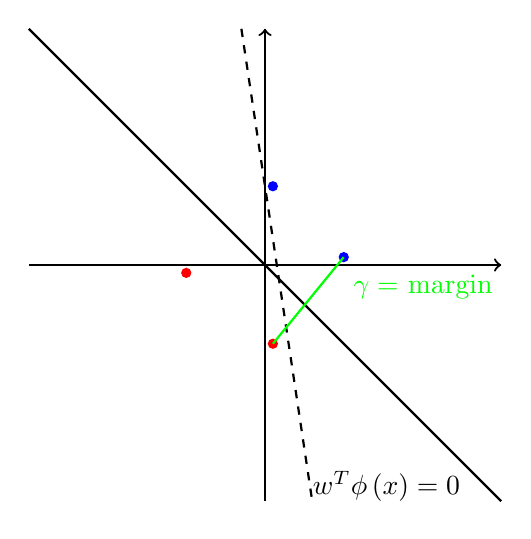
\begin{tikzpicture} [scale = 1] 
\draw[->, thick] (-3.0, 0.0) -- (3.0, 0.0);
\draw[->, thick] (0.0, -3.0) -- (0.0, 3.0);
\draw[thick] (-3.0, 3.0) -- (3.0, -3.0);
\draw[blue, fill=blue, thick] (0.1, 1.0) circle [radius = 0.05];
\draw[blue, fill=blue, thick] (1.0, 0.1) circle [radius = 0.05];
\draw[red, fill=red, thick] (-1.0, -0.1) circle [radius = 0.05];
\draw[red, fill=red, thick] (0.1, -1.0) circle [radius = 0.05];
\draw[dashed, thick] (-0.3, 3.0) -- (0.6, -3.0);
\draw[green, thick] (1.0, 0.1) -- (0.1, -1.0);
\node[below left] at (2.6, -2.5){$w^{T} \phi\left(x\right) = 0$};
\node[green, below right] at (1.0, 0.0){$\gamma =$ margin};
\end{tikzpicture} \end{figure}
solid line is $\displaystyle\max$ margin separtor
\\* dashed line is separator but not $\displaystyle\max$ margin

sum of hinge losses
\begin{align*}
H\left(w\right)  &= \displaystyle\sum_{i=1}^{n} \left(1 - y_{i} w^{T} \phi\left(x_{i}\right)\right)_{+}
\end{align*}
linearly separable $\Rightarrow  \exists w \text{\;such that\;} H\left(w\right) = 0$

$\displaystyle\max$-margin separator
\\* $w $ with smallest norm
\\* and $y_{i} w^{T} \phi\left(x_{i}\right) \geq  1$ for all $i $



\subsection{$\displaystyle\max$-margin opt}
\begin{align*}
\displaystyle\min_{w} \| w \|^{2} \text{\;such that\;} y_{i} w^{T} \phi\left(x_{i}\right) &\geq  1
\\ \text{\;such that\;} \displaystyle\sum_{i=1}^{n} \left(1 - y_{i} w^{T} \phi\left(x_{i}\right)\right)_{+} &= 0
\end{align*}
Lagrangian form:
\begin{align*}
&\displaystyle\min_{w} \displaystyle\sum_{i=1}^{n} \left(1 - y_{i} w^{T} \phi\left(x_{i}\right)\right)_{+} + \underbrace{\lambda}_{\text{\;Lagrange mult\;}} \| w \|^{2}
\end{align*}
for $\lambda > 0$ tiny



\subsection{Perceptron}
\begin{align*}
\left\{\left(x_{i}, y_{i}\right)\right\} \hat{y}_{i} &= \text{sign}\left(w^{T} x_{i}\right)
\\ w_{1} &= \text{\;init\;}
\\ w_{t+1} &= w_{t} + \mu \underbrace{\left(y_{i_{t}} - \hat{y}_{i_{t}}\right)}_{\text{\;error\;}} x_{i_{t}}, t \geq  1
\\ y &= 1, w^{T} x > 0
\end{align*}
\[ y - \hat{y} =\left\{ \begin{array}{ll}
0& \text{\;if\;} y = 1, w^{T} x > 0 \\
0& \text{\;if\;} y = -1, w^{T} x < 0 \\
2& \text{\;if\;} y = 1, w^{T} x < 0 \\
-2& \text{\;if\;} y = -1, w^{T} x > 0 \\
\end{array}\right. \]
\[ y - \hat{y} =\left\{ \begin{array}{ll}
0& \text{\;if\;} y w^{T} x > 0 \\
2 y& \text{\;if\;} y w^{T} x < 0 \\
\end{array}\right. \]
\begin{align*}
w_{t+1} &= w_{t} + \mu \left(2 y_{i_{t}}\right) \mathbbm{1}_{\left\{y_{i_{t}} w_{t}^{T} x_{i_{t}} < 0\right\}} x_{i_{t}}
\\ &= w_{t} + 2 \mu \mathbbm{1}_{\left\{y_{i_{t}} w_{t}^{T} x_{i_{t}} < 0\right\}} y_{i_{t}} x_{i_{t}}
\end{align*}
SGD with loss function $l $ with derivative $l'$
\begin{align*}
w_{t+1} &= w_{t} + \gamma \left(-l'\left(y_{i_{t}} w_{t}^{T} x_{i_{t}}\right)\right) y_{i_{t}} x_{i_{t}}
\\ &= w_{t} - \gamma \dfrac{\partial l}{\partial w} \bigg|_{w = w_{t}}
\\ \gamma &= 2 \mu
\end{align*}
-$l'\left(z\right) = \mathbbm{1}_{\left\{z < 0\right\}}$
\\* $\hat{y} = f\left(w^{T} x\right)$, single layer perceptron



\subsection{Multilayer Neural Network}
\begin{align*}
\hat{y} &= W_{L} f\left(W_{L-1} ... \left(W_{2} f\left(W_{1} x + b_{1}\right) + b_{2}\right) + ... + b_{L-1}\right) + b_{L}
\end{align*}
$W  x$ affine linear map
\\* $f\left(\cdot \right) $ nonlinear coodinate-wise
\\* $f\left(v\right)  = \begin{bmatrix} f\left(v_{1}\right) \\ ... \\ f\left(v_{n}\right) \end{bmatrix}, v \in \mathbb{R}^{n}$, "activation" function
\begin{align*}
&\displaystyle\min_{\left(w_{j}, b_{j}\right)_{j=1}^{L}} \displaystyle\sum_{i=1}^{n} l\left(y_{i} \hat{y}_{i}\left(\left\{w_{j}, b_{j}\right\}\right)\right)
\end{align*}


\subsection{Two-Layer Neural Net}
\begin{align*}
\hat{y} &= W_{2} f\left(W_{1} + b_{1}\right) + b_{2}
\end{align*}
linear in $W_{2}, b_{2}$, but nonlinear in $w_{1}, b_{1}$



\subsection{Kernel Machine $= 2$ Layer Net}
\begin{align*}
\hat{y} &= \displaystyle\sum_{i=1}^{n} \alpha_{i} K\left(x_{i}, x\right)
\end{align*}
linear  in parameter
\begin{align*}
W_{2} &= \begin{bmatrix} \alpha_{1} & ... & \alpha_{n} \end{bmatrix}
\\ K\left(x_{i}, x\right)  &= f\left(x_{i}^{T} + b_{i}\right)
\end{align*}
\begin{eg} \label{eg:km1} 
$\left(w_{i}^{T} x + 1\right)^{k}, f\left(\cdot \right) = \left(\cdot \right)^{k}$
\end{eg}
\begin{eg} \label{eg:km2} 
$\exp\left(x_{i}^{T} x\right), f\left(\cdot \right) = \exp\left(\cdot \right)$
\end{eg}
\begin{eg} \label{eg:km3} 
$\exp\left(- \dfrac{1}{2} \| x_{i} - x \|^{2}\right) = \exp\left(x_{i}^{T} x - \underbrace{\dfrac{1}{2} \left(\| x \|^{2}  + \| x_{i} \|^{2}\right)}_{b_{1}}\right)$
\end{eg}
\begin{align*}
W_{1}^{T} &= \begin{bmatrix} x_{1} & ... & x_{n} \end{bmatrix}
\\ \hat{y} &= W_{2} f\left(W_{1} x + b_{1}\right)
\\ &\begin{bmatrix} x_{1}^{T} x \\ ... \\ x_{n}^{T} x \end{bmatrix}
\end{align*}


\subsection{Difference}
$W_{1}, b_{1}$ fixed for kernel machine
\\* layer $1$ width $= n $
\\* Kernel machines are neural nets

Variable parameter for neural net
\\* layer $2$ width $=$ anything
\\* But note all neural nets are kernal mahines







\section{Lecture $23$} 

\subsection{Two-Layer NNs}
\begin{align*}
y  &= W_{2} f \left(W_{1} x + b_{1}\right)
\end{align*}
$W_{1}, b_{1}$ are fixed in kernel



\subsection{Convolutions NNs}
$1$ network layer (in general)
\begin{align*}
y  &= f\left(w_{i}^{T} x + b_{i}\right)
\\ W_{1} &= \begin{bmatrix} w_{1}^{T} \\ w_{2}^{T} \\ ... \\ w_{n}^{T} \end{bmatrix}
\end{align*}
CNN
\begin{align*}
y_{i} &= f\left(\| w_{i} \star x \|_{\infty} - b_{i}\right)
\end{align*}
convolution
\begin{align*}
\left(w_{i} \star x\right)_{k} &= \displaystyle\sum_{j=1}^{d} w_{ij} x_{k-j}
\end{align*}
$\displaystyle\max$ pooling: $\displaystyle\max$ output of conv
\begin{align*}
&\| w_{i} \star x \|_{\infty}
\\ f\left(z\right)  &= \displaystyle\max\left\{0, z \right\}
\end{align*}


\subsection{Backprop  $=$ SGD}



\subsection{Stone-Weierstrauss Thm (informal)}
any continuous function $\left[0, 1\right]^{d}$ can be approximated point-wise to arbitrary accurracy with a polynomial.
\begin{thm} \label{thm:sw} 
for any continuous $f $ on $\left[0, 1\right]^{d}$ there exists a neural net
\begin{align*}
g\left(x\right)  &= W_{2} f\left(W_{1} x\right)
\\ &W_{1} \in \mathbb{R}^{D \times d}
\\ f\left(u_{i}^{T} x\right)  &= \left(u_{i}^{T} + 1\right)^{k}
\\ W_{1} &= \begin{bmatrix} u_{1}^{T} \\ ... \\ u_{n}^{T} \end{bmatrix}
\end{align*}
for $k $ and $n $ sufficiently large, $n  = D $ and
\begin{align*}
&u_{i} \in \mathbb{R}^{d}
\\ &u_{i} \stackrel{iid}{\sim} p 
\end{align*}
where $p $ is any continuous density on $\left[0, 1\right]^{d}$
\end{thm}
Example:
\begin{align*}
&g  : \mathbb{R}^{d} \to  \mathbb{R}
\\ g\left(x\right)  &= v^{T} f\left(W, x \right)
\\ &= v^{T} \begin{bmatrix} \left(v_{1}^{T} x + 1\right)^{k} \\ ... \\ \left(v_{n}^{T} x + 1\right)^{k} \end{bmatrix}
\\ &= v^{T} \begin{bmatrix} \phi\left(u_{1}\right)^{T} \phi\left(x\right) \\ ... \\ \phi\left(u_{n}\right)^{T} \phi\left(x\right) \end{bmatrix}
\\ \phi\left(x\right) \in \mathbb{R}^{D}, D &= \dbinom{d+k}{k}
\\ g\left(x\right)  &= \displaystyle\sum_{i=1}^{n} v_{i} \phi\left(u_{i}\right)^{T} \phi\left(x\right)
\\ &= \left(\Phi^{T} v\right)^{T} \phi\left(x\right)
\\ &= w^{T} \phi\left(x\right)
\\ \Phi^{T} &= \begin{bmatrix} \phi\left(u_{1}\right) & ... & \phi\left(u_{D}\right) \end{bmatrix}
\end{align*}
general polynomial
\\* If $\Phi^{T}$ is invertible
\begin{align*}
v  &= \left(\Phi^{T}\right)^{-1} w 
\end{align*}
\begin{lem} \label{lem:polyf} 
If $h  : \mathbb{R}^{d} \to  \mathbb{R}$ is a polynomial function $\neq  0$ and if $u  \in \mathbb{R}^{d}$ is a continuous random point, then $\mathbb{P}\left\{h\left(u\right) = 0\right) = 0$
\end{lem}
Intuition:
\begin{align*}
&\phi\left(u_{1}\right) \in \mathbb{R}^{D}
\end{align*}
$v_{1}, ..., v_{D-1}$ be a basis for othogonal subspace
\begin{align*}
&  \phi\left(u_{2}\right)
\\ &  \mathbb{P}\left\{v_{j}^{T} \phi\left(u_{2}\right) = 0\right\} = 0
\\ &\Rightarrow  \phi\left(u_{2}\right) \text{\;is linearly independent of\;} \phi\left(u_{1}\right)
\end{align*}





\section{Lecture $24$} 

\subsection{Probably Approx Correct Learning}
$\mathcal{X} =$ feature space, $\mathcal{X} = \mathbb{R}^{d}, \hat{y} = f\left(x\right), f \in \mathcal{F}$
\\* $\mathcal{Y} =$ label space, $\mathcal{Y} = \left\{-1, +1\right\}$
\\* $\mathcal{F} =$ hypothesis space, $\mathcal{F} = \left\{\text{\;linear classifiers\;}\right\}$
\\* $l  =$ loss function, $l  : \mathcal{Y} \times \mathcal{Y} \mathbb{R}_{+}$



\subsection{Empirical Risk Minimization (ERM)}
\begin{align*}
\hat{f} &= \arg\displaystyle\min_{f \in \mathcal{F}} \dfrac{1}{n} l\left(y_{i}, f\left(x_{i}\right)\right)
\\ &\left\{\left(x_{i}, y_{i}\right)\right\}_{i=1}^{n} \stackrel{iid}{\sim} P 
\end{align*}
Emp Risk:
\begin{align*}
\hat{R}\left(f\right) &= \dfrac{1}{n} \displaystyle\sum_{i=1}^{n} l\left(y_{i}, f\left(x_{i}\right)\right)
\end{align*}
True Risk:
\begin{align*}
R\left(f\right)  &= \mathbb{E}_{\left(x_{i}, y_{i}\right) \sim  P} \left[l\left(y, f\left(x\right)\right)\right]
\\ f^\star  &= \arg\displaystyle\min_{f \in \mathcal{F}} R\left(f \right)
\end{align*}
Want $\hat{R}\left(f\right) \approx R\left(f \right)$ for all $f $, uniformly close
\begin{align*}
\mathbb{P}\left\{| \hat{R}\left(f\right) - R\left(f\right) | \geq  t\right\} &\leq  \mathbb{P}\left\{| \hat{R}\left(f\right) - R\left(f\right) |^{2} \geq  t^{2}\right\}
\\ &\leq  \dfrac{\mathbb{E}\left[\left(\hat{R}\left(f\right) - R\left(f\right)\right)^{2}\right]}{t^{2}}
\\ &= \dfrac{\mathbb{V}\left[\hat{R}\left(f\right)\right]}{t^{2}}
\\ &\leq  \dfrac{c^{2}}{4 n t^{2}}
\end{align*}
Markov's Inequality
\begin{align*}
\hat{R}\left(f\right) &= \dfrac{1}{n} \left(\displaystyle\sum_{i=1}^{n} \left[\underbrace{l\left(y_{i}, f\left(x_{i}\right)\right]}_{\text{\;bounded by\;} c }\right)\right.
\\ 0 &\leq  l \leq  c
\end{align*}
$l = 0$ with probability $\dfrac{1}{2}$
\\* $l = c$ with porbability $\dfrac{1}{2}$
\begin{align*}
&\Rightarrow  \mathbb{V}\left[l\right] \leq  \dfrac{c^{2}}{4}
\end{align*}


\subsection{Chernoff's Bound}
\begin{align*}
&\mathbb{P}\left\{\hat{R}\left(f\right) - R\left(f\right) \geq  t\right\}
\\ \mathbb{P}\left\{e^{\lambda \left(\hat{R}\left(f\right) - R\left(f\right)\right)} \geq  e^{\lambda t}\right\} &\leq  e^{-\lambda t} \mathbb{E}\left[e^{\lambda \left(\hat{R}\left(f\right) - R\left(f\right)\right)}\right]
\\ \mathbb{P}\left\{\hat{R}\left(f\right) - R\left(f\right) \geq  t\right) &\leq  e^{- \dfrac{2 n t^{2}}{c^{2}}}
\\ \mathbb{P}\left\{| \hat{R}\left(f\right) - R\left(f\right) | \geq  t\right\} &= \mathbb{P}\left\{\hat{R}\left(f\right) - R\left(f\right) \geq  t \text{\;or\;} R\left(f\right) - \hat{R}\left(f\right) \geq  t\right)
\\ &\leq  2 e^{- \dfrac{2 n t^{2}}{c^{2}}}
\end{align*}
by union bound
\begin{align*}
\mathbb{P}\left\{ \hat{R}\left(f_{1}\right) - R\left(f_{1}\right) \geq  t \text{\;or\;} \hat{R}\left(f_{2}\right) - R\left(f_{2}\right) \geq  t \text{\;or\;} ...\right\} &\leq  \text{\;small bound\;}
\end{align*}
Assume $\mathcal{F}$ is finte.
\\* $k  = | \mathcal{F} |$ is the number of classifiers in $\mathcal{F}$.



\subsection{Uniform Bound}
\begin{align*}
&\mathbb{P}\left\{ \hat{R}\left(f_{1}\right) - R\left(f_{1}\right) \geq  t \text{\;or\;} \hat{R}\left(f_{2}\right) - R\left(f_{2}\right) \geq  t \text{\;or\;} ... \underbrace{\hat{R}\left(f_{k}\right) - R\left(f_{k}\right) \geq  t}_{\text{\;bad things\;}}\right\}
\\ &\leq  \displaystyle\sum_{i=1}^{k} \left\{ | \hat{R}\left(f_{i}\right) - R\left(f_{i}\right) | \geq  t \right\}, \text{\;union bound\;}
\\ &\leq  \underbrace{| \mathcal{F} | 2 e^{- \dfrac{2 n t^{2}}{c^{2}}}}_{\delta}
\\ \delta &= 2 | \mathcal{F} | e^{- \dfrac{2 n t^{2}}{c^{2}}}
\\ \log \dfrac{2 \mathcal{|F}|}{\delta} &= \dfrac{2 n t^{2}}{c^{2}}
\\ t  &= \sqrt{\dfrac{c^{2} \log\left(\dfrac{2 \mathcal{|F}|}{\delta}\right)}{2 n}}
\end{align*}
with probabiliy $\geq  1 - \delta$,
\begin{align*}
\displaystyle\max_{f \in \mathcal{F}} | \hat{R}\left(f\right) - R\left(f\right) | &\leq  \sqrt{\dfrac{c^{2} \log\left(\dfrac{2 \mathcal{|F}|}{\delta}\right)}{2 n}}
\end{align*}
\begin{align*}
f^\star  &= \arg\displaystyle\min_{f \in \mathcal{F}} \mathbb{E}\left[l\left(y, f\left(x\right)\right)\right]
\\ &= \arg\displaystyle\min_{f \in \mathcal{F}} R\left(f\right) 
\\ \hat{f} &= \arg\displaystyle\min_{f \in \mathcal{F}} \dfrac{1}{n} \displaystyle\sum_{i=1}^{n} l\left(y_{i}, f\left(x_{i}\right)\right)
\\ &= \arg\displaystyle\min_{f \in \mathcal{F}} \hat{R}\left(f\right)
\\ R\left(\hat{f}\right)  &\leq  \hat{R}\left(\hat{f}\right) + \sqrt{\dfrac{c^{2} \log\left(\dfrac{2 \mathcal{|F}|}{\delta}\right)}{2 n}} \text{\;wp\;} \geq  1 - \delta
\\ &\leq  \hat{R}\left(f^\star \right) + \sqrt{\dfrac{c^{2} \log\left(\dfrac{2 \mathcal{|F}|}{\delta}\right)}{2 n}}, \text{\;since\;} \hat{f} \displaystyle\min \hat{R}
\\ &\leq  R\left(f^\star \right) + \sqrt{\dfrac{c^{2} \log\left(\dfrac{2 \mathcal{|F}|}{\delta}\right)}{n}}
\end{align*}
Generalization Bound

decreases like $\dfrac{1}{\sqrt{n}}$
\\* inreases with $\log\left(\dfrac{1}{\delta}\right)$ and $\log | \mathcal{F} |$
\begin{align*}
n  &\geq  \log | \mathcal{F} |
\\ \Delta &= \displaystyle\min_{f \neq  f^\star } R\left(f\right) - R\left(f^\star \right)
\end{align*}
with prob $\geq  1 - \delta$
\begin{align*}
R\left(\hat{f}\right)  &\leq  R\left(f^\star \right) + \sqrt{\dfrac{2 \log\left(\dfrac{2 \mathcal{|F}|}{\delta}\right)}{n}}
\\ \mathbb{E}\left[R\left(\hat{f}\right)\right] &\leq  \left(1 - \delta\right) \left[R\left(f^\star \right) + \sqrt{\dfrac{2 \log\left(\dfrac{2 \mathcal{|F}|}{\delta}\right)}{n}}\right] + \delta c , \text{\;take\;} \delta = \dfrac{1}{\sqrt{n}}
\\ &\leq  R\left(f^\star \right) + \tilde{O}\left(\sqrt{\dfrac{\log \mathcal{|F}| + \log n}{n}}\right)
\end{align*}


\subsection{Infinite $\mathcal{F}$}
\begin{align*}
\mathcal{F} &= \left\{\text{\;all linear classifiers on\;} \left[0, 1\right]^{k}\right\}
\\ | \mathcal{F}_{\varepsilon} | &= o\left(\left(\dfrac{1}{\varepsilon}\right)^{d}\right)
\\ &\log | \mathcal{F}_{\varepsilon} | \sim  d \log \dfrac{1}{\varepsilon}
\\ t  &= \sqrt{\dfrac{c^{2} \log\left(\dfrac{2 \mathcal{|F}|}{\delta}\right)}{n}}
\end{align*}


\subsection{Hyperparameter Tuning}
\begin{align*}
\hat{w}_{\lambda} &= \arg\displaystyle\min_{w \in \mathbb{R}^{d}} \displaystyle\sum_{i=1}^{n} \left(1 - y_{i} w^{T} x_{i}\right)_{+} \lambda \| w \|^{2}, \lambda \in \Lambda
\end{align*}
want "tune" $\lambda$
\begin{align*}
&\left\{\left(x_{i}, y_{i}\right)\right\}_{i=1}^{n}
\\ n &= n_{T} + n_{H}
\\ w_{\lambda} &= \arg\displaystyle\min \displaystyle\sum_{i=1}^{n_{T}} \left(1 - y_{i} w^{T} x_{i}\right)_{+} + \lambda \| w \|^{2}
\end{align*}
use hold out set $\left\{\left(x_{i}, y_{i}\right)\right\}_{i = n_{T} + 1}^{n}$ validate, tune $\lambda$
\begin{align*}
\hat{R}\left(w_{\lambda}\right) &= \dfrac{1}{n_{H}} = \displaystyle\sum_{i = n_{T} + 1}^{n} \mathbbm{1}_{\left\{y_{i} w^{T}_{\lambda} x_{i} < 0\right\}}
\end{align*}
number of mistakes $w_{\lambda}$ makes on hold out
\begin{align*}
\lambda^\star  &= \arg\displaystyle\min_{\lambda \in \Lambda} \mathbb{E}\left[\mathbbm{1}_{\left\{y w_{\lambda}^{T} x < 0\right\}}\right]
\\ \hat{\lambda} &= \arg\displaystyle\min_{\lambda \in \Lambda} \hat{R}\left(w_{\lambda}\right)
\end{align*}
Assume $\Lambda$ is finite
\begin{align*}
\Lambda &= \left\{\lambda_{1}, \lambda_{2}, ..., \lambda_{k}\right\}
\\ | \hat{R}\left(w_{\lambda}\right) - R\left(w_{\lambda}\right) | &\leq  \sqrt{\dfrac{2 \log \dfrac{2 | \Lambda |}{\delta}}{n_{H}}}, \text{\;wp\;} \geq  1 - \delta
\end{align*}





\section{Lecture $25$} 
Feature space $\mathcal{X}$
\\* Label sapce $\mathcal{Y}$
\\* Predictor $f  : \mathcal{X} \to  \mathcal{Y}, f \in \mathcal{F}$
\\* Loss function $l  : l : \mathcal{Y} \times \mathcal{Y} \to  \left[0, \infty\right)$
\begin{align*}
&\left\{\left(x_{i}, y_{i}\right)\right\}_{i = 1, 2, ..., n} \stackrel{iid}{\sim} P 
\\ R\left(f\right)  &= \mathbb{E}_{\left(x, y\right) \sim  P}\left[l\left(y, f\left(x\right)\right)\right]
\\ \hat{R}_{n}\left(f\right) &= \dfrac{1}{n} \displaystyle\sum_{i=1}^{n} l\left(y_{i}, f\left(x_{i}\right)\right)
\\ f^\star  &= \arg\displaystyle\min_{f \in \mathcal{F}} R\left(f\right) 
\\ \hat{f} &= \arg\displaystyle\min_{f \in \mathcal{F}} \hat{R}\left(f\right)
\\ &  \mathbb{P}\left\{| R\left(\hat{f}\right) - R\left(f^\star \right) | \geq  t\right\}
\\ &\leq  2 | \mathcal{F} | \exp\left(- \dfrac{2 n t^{2}}{c^{2}}\right)
\\ t &< \sqrt{\dfrac{\log | \mathcal{F} | + \log n}{n}}
\end{align*}

\subsection{Markov Ineq}
$X  > 0, \phi$ increasing
\begin{align*}
\mathbb{P}\left\{\phi\left(X\right) > \phi\left(t\right)\right\} &= \mathbb{P}\left\{X \geq  t\right\} \leq  \dfrac{\mathbb{E}\left[X\right]}{t}
\\ \mathbb{E}\left[X\right] &\geq  \mathbb{E}\left[X \mathbbm{1}_{\left[X \geq  t\right]}\right] \geq  \mathbb{E}\left[t \mathbbm{1}_{\left[X \geq  t\right]}\right] = t \mathbb{P}\left\{X \geq  t\right\}
\end{align*}


\subsection{Chebyshev Inequality}
\begin{align*}
&  \mathbb{P}\left\{| X - \mathbb{E}\left[X\right] | \geq  t\right\}
\\ &= \mathbb{P}\left\{| X - \mathbb{E}\left[X\right] |^{2} \geq  t^{2}\right\}
\\ &\leq  \dfrac{\mathbb{V}\left[X\right]}{t^{2}}
\end{align*}


\subsection{Cherboeff Bound}
\begin{align*}
&  \mathbb{P}\left\{X - \mathbb{E}\left[X\right] \geq  t\right\}
\\ &= \mathbb{P}\left\{\exp\left(s \left(X - \mathbb{E}\left[X\right]\right)\right) \geq  e^{s t}\right\}
\\ &\leq  \dfrac{\mathbb{E}\left[\exp\left(s \left(X - \mathbb{E}\left[X\right]\right)\right)\right]}{e^{s t}}
\\ &\leq  \displaystyle\min_{s > 0} \dfrac{\mathbb{E}\left[e^{s X}\right]}{e^{s t} e^{s \mathbb{E}\left[X\right]}}
\end{align*}


\subsection{Sub Gaussian Random Variables}
Assume $\mathbb{E}\left[X\right] = 0$,
\begin{align*}
\mathbb{E}\left[e^{s X}\right] &\leq  e^{\dfrac{c s^{2}}{2}}, c > 0
\\ \mathbb{P}\left\{| X | \geq  t\right\} &\leq  \dfrac{e^{\dfrac{c s^{2}}{2}}}{e^{s t}} = e^{\dfrac{c s^{2}}{2} - s t}
\\ &\leq  e^{- \dfrac{t^{2}}{2 c}}
\\ s  &= \dfrac{t}{c}
\end{align*}
X is subGaussian with param $c, $
\begin{align*}
S_{n} &= \displaystyle\sum_{i=1}^{n} x_{i}
\\ \mathbb{E}\left[e^{s S_{n}}\right] &= \mathbb{E}\left[e^{s \displaystyle\sum_{i=1}^{n} x_{i}}\right]
\\ &= \displaystyle\prod_{i=1}^{n} \mathbb{E}\left[e^{s X_{i}}\right] \leq  \exp\left(\dfrac{n c s^{2}}{2}\right)
\\ \mathbb{P}\left\{ | S_{n} | \geq  t\right\} &\leq  \exp\left(- \dfrac{t^{2}}{2 n c}\right)
\\ \mathbb{P}\left\{ \dfrac{|1}{n} \displaystyle\sum x_{i} | \geq  t\right\} &\leq  \exp\left(- \dfrac{n t^{2}}{2 c}\right)
\end{align*}
X is bounded, $x  \in \left[a, b \right]$
\begin{align*}
\mathbb{E}\left[e^{s X}\right] &\leq  e^{\dfrac{\left(b - a\right)^{2} s^{2}}{2}}
\end{align*}


\subsection{Shattering Coefficient of $\mathcal{F}$}
\begin{align*}
D_{n} &= \left\{\left(x_{i}, y_{i}\right)\right\}_{i = 1, ..., n}
\\ \mathcal{S}\left(\mathcal{F}, n\right) &= \displaystyle\max_{x_{1}, ..., x_{n}} \left| \left\{\left(f\left(x_{1}\right), f\left(x_{2}\right), ..., f\left(x_{n}\right)\right), f \in \mathcal{F}\right\} \right|
\end{align*}
Examples:
\\* $\mathcal{F}: 1$-dim linear classifier
\begin{align*}
\mathcal{F}_{D_{n}} &= \left\{\left(+, +, +\right), \left(-, -, -\right), \left(+, -, -\right), \left(-, -, +\right), \left(-, +, +\right), \left(+, +, -\right)\right\}
\\ VC  \left(\mathcal{F}\right) &\geq  2
\end{align*}
$\mathcal{F}': 2$-dim linear classifier
\begin{align*}
\mathcal{F}_{D_{n}} &= \left\{-1, +1\right\}^{3}
\\ VC  \left(\mathcal{F}\right) &\geq  3
\end{align*}
The total number of classifiers is,
\begin{align*}
&2 \dbinom{n}{d}
\end{align*}
$\mathcal{F}$ shatter $D_{n}$ if $\mathcal{F}_{D_{n}}$ contains all tuples of $\left\{+1, -1 \right\}^{n} \Rightarrow  | \mathcal{F}_{D_{n}} | = 2^{n}$ .
\\* $VC  \left(\mathcal{F}\right) = k $ if $k $ is the largest integer there exist $D_{k}$ such that $\mathcal{F}$ shatter $D_{k}$
\\* VC of $d $ dim linear classifiers is $d  + 1$



\subsection{FTSLT}
\begin{align*}
\mathbb{P}\left\{\displaystyle\sup_{f \in \mathcal{F}} | \hat{R}_{n}\left(f\right) - R\left(f\right) | \geq  \varepsilon\right\} &\leq  8 \mathcal{S}\left(\mathcal{F}, n\right) e^{- \dfrac{n \varepsilon^{2}}{32}}
\\ &= O\left(e^{0 \dfrac{n \varepsilon^{2}}{c} + VC  \log n}\right)
\\ \mathcal{S}\left(\mathcal{F}, n\right) &\leq  \left(n + 1\right)^{VC }
\end{align*}
\begin{align*}
D_{n} &= \left\{\left(x_{i}, y_{i}\right)\right\}_{i = 1, ..., n}
\\ D'_{n} &= \left\{\left(x'_{i}, y'_{i}\right)\right\}_{i = 1, ..., n}
\\ \hat{R} '_{n}\left(f\right) &= \dfrac{1}{n} \displaystyle\sum_{i=1}^{n} \mathbbm{1}_{\left[f\left(x'_{i}\right) \neq  y_{i}\right]}
\end{align*}
Step $1$:
\begin{align*}
\mathbb{P}\left\{\displaystyle\sup_{f \in \mathcal{F}} | \hat{R}_{n}\left(f\right) - R\left(f\right) | \geq  \varepsilon\right\} &\leq  2 \mathbb{P}\left\{\displaystyle\sup_{f \in \mathcal{F}} | \hat{R}_{n}\left(f\right) - \hat{R} '_{n}\left(f\right) | > \dfrac{\varepsilon}{2}\right\}
\end{align*}
\[ \left\{\sigma_{i}\right\}_{i = 1, ..., n} =\left\{ \begin{array}{ll}
+1& \text{\;with probability\;} \dfrac{1}{2} \\
-1& \text{\;with probability\;} \dfrac{1}{2} \\
\end{array}\right. \]
\begin{align*}
&  \mathbb{P}\left\{\displaystyle\sup_{f \in \mathcal{F}} | \hat{R}_{n}\left(f\right) - \hat{R} '_{n}\left(f\right) | > \dfrac{\varepsilon}{2}\right\}
\\ &= \mathbb{P}\left\{\displaystyle\sum_{f \in \mathcal{F}} \dfrac{1}{n} \left| \displaystyle\sum_{i=1}^{n} \sigma_{i} \left(\mathbbm{1}_{\left\{f\left(x_{i}\right) \neq  y_{i}\right\}} - \mathbbm{1}_{\left\{f\left(x'_{i}\right) \neq  y'_{i}\right\}}\right) \right| \geq  \dfrac{\varepsilon}{2}\right\}
\\ &\leq  \mathbb{P}\left\{\displaystyle\sum_{f \in \mathcal{F}} \dfrac{1}{n} \left| \displaystyle\sum_{i=1}^{n} \sigma_{i} \left(\mathbbm{1}_{\left\{f\left(x_{i}\right) \neq  y_{i}\right\}}\right) \right| \geq  \dfrac{\varepsilon}{4}\right\} + \mathbb{P}\left\{\displaystyle\sum_{f \in \mathcal{F}} \dfrac{1}{n} \left| \displaystyle\sum_{i=1}^{n} \sigma_{i} \left(\mathbbm{1}_{\left\{f\left(x'_{i}\right) \neq  y'_{i}\right\}}\right) \right| \geq  \dfrac{\varepsilon}{4}\right\}
\\ &  \mathbb{P}\left\{\displaystyle\sum_{f \in \mathcal{F}} \dfrac{1}{n} \left| \displaystyle\sum_{i=1}^{n} \sigma_{i} \left(\mathbbm{1}_{\left\{f\left(x_{i}\right) \neq  y_{i}\right\}}\right) \right| \geq  \varepsilon\right\}
\\ &= \mathbb{E}\left[\mathbbm{1}_{\left\{ \displaystyle\sup_{f \in \mathcal{F}_{D_{n}}} \dfrac{1}{n} \left| \displaystyle\sum_{i=1}^{n} \sigma_{i} \left(\mathbbm{1}_{\left\{f\left(x_{i}\right) \neq  y_{i}\right\}}\right) \right| \geq  \varepsilon \right\}} | D_{n}\right]
\\ &\leq  \mathcal{S}\left(\mathcal{F}, n\right) \mathbb{E}\left[\displaystyle\sup_{f \in \mathcal{F}} \mathbb{P}\left\{\dfrac{1}{n} \left| \displaystyle\sum_{i=1}^{n} \underbrace{\sigma_{i} \left(\mathbbm{1}_{\left\{f\left(x_{i}\right) \neq  y_{i}\right\}}\right)}_{iid, bounded by 1, expecation 0} \right| \geq  \varepsilon | D_{n}\right\}\right.
\\ &\leq  \mathcal{S}\left(\mathcal{F}, n\right) e^{- \dfrac{n \varepsilon^{2}}{32}}
\end{align*}





\section{Lecture $26$} 
\begin{align*}
R\left(f\right)  &= \mathbb{P}\left\{f\left(X\right) \neq  y\right\}
\\ \hat{R}\left(f\right) &= \dfrac{1}{n} \displaystyle\sum_{i=1}^{n} \mathbbm{1}_{\left\{f\left(x_{i}\right) \neq  y_{i}\right\}}
\\ f  \in \mathcal{F}, \hat{f} &= \arg\displaystyle\min_{f \in \mathcal{F}} \hat{R}\left(f\right)
\\ f^\star  &= \arg\displaystyle\min_{f \in \mathcal{F}} R\left(f\right) 
\end{align*}

\subsection{Uniform Derivation Bound}
\begin{align*}
\displaystyle\sup_{f \in \mathcal{F}} | R\left(f\right) - \hat{R}_{n} \left(f\right) | &\leq  6 \sqrt{\dfrac{\underbrace{d_{\mathcal{F}}}_{VC dim\left(\mathcal{F}\right)} \log\left(\dfrac{n}{\delta}\right)}{n}} \text{\;wp\;} \geq  1 - \delta
\\ R\left(\hat{f}\right)  &\leq  \hat{R}\left(\hat{f}\right) + 6 \sqrt{\dfrac{d_{\mathcal{F}} \log\left(\dfrac{n}{\delta}\right)}{n}}
\\ &\leq  \hat{R}\left(f^\star \right) + 6 \sqrt{\dfrac{d_{\mathcal{F}} \log\left(\dfrac{n}{\delta}\right)}{n}}
\\ &\leq  R\left(\hat{f}\right) + 12 \sqrt{\dfrac{d_{\mathcal{F}} \log\left(\dfrac{n}{\delta}\right)}{n}}
\end{align*}
generalization bound



\subsection{VC Dimensions}
VC dim of axis-aligned rectangles in $\mathbb{R}^{d} = 2 d $



\subsection{Sample Complexity}
\begin{align*}
n  &>> d_{\mathcal{F}}
\end{align*}


\subsection{Neural nets}
VC dim of $L $ layer ReLU $= O\left(L \cdot  W\right) $
\\* $W $ is total number of weights $\neq  d $
\\* $L $ is number of layers



\subsection{Cross Validation}
hold out $\dfrac{n}{10}$
\begin{align*}
\hat{f} &= \arg\displaystyle\min_{\dfrac{9}{10} n}
\\ R\left(\hat{f}\right)  &\leq  \hat{R}\left(\hat{f}\right) + \sqrt{\dfrac{2 \log\left(\dfrac{1}{\delta}\right)}{n}}
\end{align*}
Chernoff bound



\subsection{Convex Loss Functions}
\begin{align*}
l\left(z\right)  &= \left(1 - z\right)_{+}
\\ \mathbb{P}\left\{\text{\;err\;} \right\} &\leq  R\left(f\right) = \mathbb{E}\left[\hat{l}\left(y f\left(x\right)\right)\right]
\\ \hat{R}\left(f\right) &= \dfrac{1}{n} \displaystyle\sum_{i=1}^{n} l\left(y_{i} f\left(x_{i}\right)\right)
\\ \hat{f}&= \arg\displaystyle\min_{f \in \mathcal{F}} \hat{R}\left(f\right)
\\ f^\star  &= \arg\displaystyle\min_{f \in \mathcal{F}} R\left(f\right) 
\end{align*}


\subsection{Linear Classifiers}
\begin{align*}
f\left(x\right)  &= w^{T} x 
\\ &\displaystyle\min_{w \in \mathbb{R}^{d}} \displaystyle\sum_{i=1}^{n} \left(1 - y_{i} w^{T} x_{i}\right)_{+}
\\ \displaystyle\sup_{f \in \mathcal{F}} | R\left(f\right) - \hat{R}\left(f\right) | &\leq  \mathbb{E}\left[\displaystyle\sup_{f \in \mathcal{F}} | R\left(f\right) - \hat{R}\left(f\right) |\right] + \sqrt{\dfrac{2 \log \dfrac{1}{\delta}}{n}} \text{\;wp\;} 1 - \delta
\end{align*}
McDiramid's Inequality



\subsection{Rademacher Complexity}
\begin{align*}
\mathbb{E}\left[\displaystyle\sup_{f} | R\left(f\right) - \hat{R}\left(f\right) |\right] &\leq  \mathbb{E}\left[\displaystyle\sup_{f} | \hat{R}'\left(f\right) - \hat{R}\left(f\right) |\right]
\\ &= \mathbb{E}\left[\displaystyle\sup_{f} \dfrac{1}{n} | \displaystyle\sum_{i=1}^{n} \left(l\left(y'_{i} f\left(x'_{i}\right)\right) - l\left(y_{i} f\left(x_{i}\right)\right)\right) |\right]
\\ &= \mathbb{E}\left[\displaystyle\sup_{f} \dfrac{1}{n} \sigma_{i} \left(\left(l\left(y'_{i} f\left(x'_{i}\right)\right) - l\left(y_{i} f\left(x_{i}\right)\right)\right)\right) |\right]
\\ &\leq  2 \mathbb{E}\left[\displaystyle\sup_{f \in \mathcal{F}} \dfrac{1}{n} | \displaystyle\sum_{i=1}^{n} \sigma_{i} l\left(y_{i} f\left(x_{i}\right)\right) |\right]
\\ &\sigma_{i} \text{\;iid\;} \pm 1 \text{\;wp\;} \dfrac{1}{2}
\end{align*}
Rademacher Complexity $\mathcal{R}_{n}\left(\mathcal{F}\right)$

$\| x_{i} \| \leq  1$ for all $i $
\begin{align*}
\mathcal{W}_{M} &= \left\{w \in \mathbb{R}^{d} : \| w \| \leq  M \right\}
\\ &\displaystyle\min_{w \in \mathcal{W}_{M}} \displaystyle\sum_{i=1}^{n} \left(1 - y_{i} w^{T} x_{i}\right)_{+}
\\ \mathcal{R}_{n}\left(\mathcal{W}_{M}\right) &= 2 \mathbb{E}\left[\displaystyle\sup_{w \in \mathcal{W}_{n}} \dfrac{1}{n} | \displaystyle\sum_{i=1}^{n} l\left(y_{i} w^{T} x_{i}\right) |\right]
\\ &\leq  4 \mathbb{E}\left[\displaystyle\sup_{w \in \mathcal{W}_{n}} \dfrac{1}{n} | \displaystyle\sum_{i=1}^{n} \sigma_{i} y_{i} x_{i} |\right]
\\ &\leq  4 \mathbb{E}\left[\displaystyle\sup_{w \in \mathcal{W}_{n}} \dfrac{1}{n} \| M \| \| \displaystyle\sum_{i=1}^{n} \sigma_{i} x_{i} \|\right]
\\ &\leq  \dfrac{4 M}{\sqrt{n}}
\end{align*}
\begin{thm} \label{thm:nnnew} 
('$17, '18) \mathcal{F} =$ neural nets with $L $ layers, $M $, using hinge or logistic
\begin{align*}
R\left(\hat{f}\right)  &\leq  \hat{R}\left(\hat{f}\right) + O\left(\sqrt{\dfrac{L M^{2}}{n}}\right)
\end{align*}
$M $ is product of Frobenius norms of all weight matrix
\end{thm}

\newpage




\section{Problem Set $1$} 


\subsection{Q1}
No



\subsection{Q2}
No



\subsection{Q3}
Strategy $1$: completely randomized,
\begin{align*}
\mathbb{P}\left\{X = \hat{X}, Y = \hat{Y}\right\} &= \mathbb{P}\left\{X = \hat{X}\right\} \mathbb{P}\left\{Y = \hat{Y}\right\}
\\ &= \dfrac{1}{6} \dfrac{1}{6}
\\ &= \dfrac{1}{36}
\end{align*}
Strategy $2$: guess the other players number,
\begin{align*}
\mathbb{P}\left\{X = Y\right\} &= \dfrac{1}{6}
\\ &< \dfrac{1}{36}
\end{align*}
This is minimal because,
\begin{align*}
\mathbb{P}\left\{X = \hat{X}, Y = \hat{Y}\right\} &\leq  \mathbb{P}\left\{X = \hat{X}\right\}
\\ &\leq  \dfrac{1}{6}
\end{align*}





\section{Problem Set $2$} 


\subsection{Q1}
\begin{align*}
\mathbb{P}\left\{g\left(x\right) \neq  Y | X = x\right\} &= \mathbb{P}\left\{Y = 1 | X = x\right\} \mathbb{P}\left\{g\left(X\right) = 0 | X = x\right\} + \mathbb{P}\left\{Y = 0 | X = x\right\} \mathbb{P}\left\{g\left(X\right) = 1 | X = x\right\}
\\ &= \eta\left(x\right) \left(1 - \mathbb{P}\left\{g\left(X\right) = 1 | X = x\right\}\right) + \left(1 - \eta\left(x\right)\right) \mathbb{P}\left\{g\left(X\right) = 1 | X = x\right\}
\\ \mathbb{P}\left\{g\left(x\right) \neq  Y | X = x\right\} - \mathbb{P}\left\{f^\star \left(x\right) \neq  Y | X = x\right\} &= \left(2 \eta\left(x\right) - 1\right)\left(\mathbb{P}\left\{f^\star \left(x\right) = 1 | X = x\right\} - \mathbb{P}\left\{g\left(x\right) = 1 | X = x\right\}\right)
\\ &\geq  0
\end{align*}
If $\eta\left(x\right) \geq  \dfrac{1}{2}$, then,
\begin{align*}
2 \eta\left(x\right) - 1 &\geq  0
\\ \mathbb{P}\left\{f^\star \left(x\right) = 1 | X = x\right\} - \mathbb{P}\left\{g\left(x\right) = 1 | X = x\right\} &= 1 - \mathbb{P}\left\{g\left(x\right) = 1 | X = x\right\} \geq  0
\end{align*}
If $\eta\left(x\right) < \dfrac{1}{2}$, then,
\begin{align*}
2 \eta\left(x\right) - 1 &< 0
\\ \mathbb{P}\left\{f^\star \left(x\right) = 1 | X = x\right\} - \mathbb{P}\left\{g\left(x\right) = 1 | X = x\right\} &= 1 - \mathbb{P}\left\{g\left(x\right) = 1 | X = x\right\} \leq  0
\end{align*}
Therefore,
\begin{align*}
\mathbb{P}\left\{g\left(X\right) \neq  Y\right\} &= \mathbb{E}\left[\mathbb{P}\left\{g\left(X\right) \neq  Y\right\} | X\right]
\\ &\geq  \mathbb{E}\left[\mathbb{P}\left\{f^\star \left(X\right) \neq  Y\right\} | X\right]
\\ &= \mathbb{P}\left\{f^\star \left(X\right) \neq  Y\right\}
\end{align*}


\subsection{Q2}
\begin{align*}
\mathbb{E}\left[Z\right] &= \mathbb{E}\left[Z | Z < t\right] \mathbb{P}\left\{Z < t\right\} + \mathbb{E}\left[Z | Z \geq  t\right] \mathbb{P}\left\{Z \geq  t\right\}
\\ &\geq  \mathbb{E}\left[Z | Z \geq  t\right] \mathbb{P}\left\{Z \geq  t\right\}
\\ &\geq  t \mathbb{P}\left\{Z \geq  t\right\}
\end{align*}


\subsection{Q3}
Start with showing mean $= 0$,
\begin{align*}
\mathbb{E}\left[\mathbbm{1}_{f\left(X_{i}\right) \neq  Y_{i}} - p_{f}\right] &= \mathbb{P}\left\{f\left(X_{i}\right) \neq  Y_{i}\right\} - p_{f}
\\ &= 0
\end{align*}
Use Markov,
\begin{align*}
\mathbb{P}\left\{| \hat{p}_{f} - p_{f} | > \varepsilon\right\} &\leq  \dfrac{\mathbb{E}\left[\left(\hat{p}_{f} - p_{f}\right)^{2}\right]}{\varepsilon^{2}}
\\ &= \dfrac{1}{\varepsilon^{2}} \mathbb{E}\left[\left(\dfrac{1}{n} \displaystyle\sum_{i=1}^{n} \mathbbm{1}_{f\left(X_{i}\right) \neq  Y_{i}} - p_{f}\right)^{2}\right]
\\ &= \dfrac{1}{\varepsilon^{2}} \mathbb{V}\left[\dfrac{1}{n} \displaystyle\sum_{i=1}^{n} \mathbbm{1}_{f\left(X_{i}\right) \neq  Y_{i}} - p_{f}\right]
\\ &= \dfrac{1}{\varepsilon^{2}} \dfrac{1}{n^{2}} \displaystyle\sum_{i=1}^{n} \mathbb{V}\left[\mathbbm{1}_{f\left(X_{i}\right) \neq  Y_{i}} - p_{f}\right]
\\ &= \dfrac{1}{\left(n \varepsilon\right)^{2}} \displaystyle\sum_{i=1}^{n} \mathbb{E}\left[\mathbbm{1}_{f\left(X_{i}\right) \neq  Y_{i}} - 2 p_{f} \mathbbm{1}_{f\left(X_{i}\right) \neq  Y_{i}} + p_{f}^{2}\right]
\\ &= \dfrac{1}{\left(n \varepsilon\right)^{2}} \displaystyle\sum_{i=1}^{n} \left(p_{f} - p_{f}^{2}\right)
\\ &= \dfrac{p_{f} \left(1 - p_{f}\right)}{n \varepsilon^{2}}
\end{align*}


\subsection{Q4}
By convexity,
\begin{align*}
g\left(x\right)  &\geq  g\left(t\right) + g'\left(t\right)\left(x - t \right)
\\ \mathbb{E}\left[g\left(x\right)\right] &\geq  g\left(t\right) + g'\left(t\right)\left(\mathbb{E}\left[x\right] - t \right)
\end{align*}
With $t  = \mathbb{E}\left[x\right]$ and $g\left(x\right)  = x^{2}$
\begin{align*}
\mathbb{E}\left[x^{2}\right] &\geq  \mathbb{E}\left[x\right]^{2}
\end{align*}


\subsection{Q5}
\begin{align*}
\mathbb{E}\left[X\right] &= \displaystyle\sum_{k=0}^{\infty} k e^{-\lambda} \dfrac{\lambda^{k}}{k!}
\\ &= \lambda \displaystyle\sum_{k=1}^{\infty} e^{-\lambda} \dfrac{\lambda^{k-1}}{\left(k-1\right)!}
\\ &= \lambda
\end{align*}


\subsection{Q6}
\begin{align*}
\mathbb{P}\left\{X_{1} + X_{2} = n\right\} &= \displaystyle\sum_{i=0}^{n} \mathbb{P}\left\{X_{1} = i, X_{2} = n - i\right\}
\\ &= \displaystyle\sum_{m=0}^{n} e^{-\lambda_{1}} \dfrac{\lambda_{1}^{i}}{i!} e^{-\lambda_{2}} \dfrac{\lambda_{2}^{n-i}}{\left(n - i\right)!}
\\ &= e^{-\lambda_{1-\lambda_{2}}} \dfrac{1}{n!} \displaystyle\sum_{i=0}^{n} \dbinom{n}{i} \lambda_{1}^{i} \lambda_{2}^{n-i}
\\ &= e^{-\lambda_{1-\lambda_{2}}} \dfrac{\left(\lambda_{1} + \lambda_{2}\right)^{n}}{n!}
\\ \mathbb{P}\left\{X_{1} = k | X_{1} + X_{2} = n\right\} &= \dfrac{\mathbb{P}\left\{X_{1} = k, X_{1} + X_{2} = n\right\}}{\mathbb{P}\left\{X_{1} + X_{2} = n\right\}}
\\ &= \dfrac{e^{-\lambda_{1}} \dfrac{\lambda_{1}^{k}}{k!} e^{-\lambda_{2}} \dfrac{\lambda_{2}^{n-k}}{\left(n-k\right)!}}{e^{-\lambda_{1-\lambda_{2}}} \dfrac{\left(\lambda_{1} + \lambda_{2}\right)^{n}}{n!}}
\\ &= \dbinom{n}{k} \delta^{k} \left(1 - \delta\right)^{n-k}, \delta = \dfrac{\lambda_{1}}{\lambda_{1} + \lambda_{2}}
\end{align*}


\subsection{Q7}
Define $\eta\left(x, k \right) = \mathbb{P}\left\{Y = k | X = x \right\}$ for $k  = 1, ..., m $, then
\begin{align*}
f^\star \left(x\right) &= \arg\displaystyle\max_{k} \eta\left(x, k\right)
\end{align*}


\subsection{Q8}
The minimum error is $p_{f} = 1 - \mathbb{E}_{x\left[\displaystyle\max_{k} \eta\left(x, k\right)\right]}$



\subsection{Q9}
An estimator is,
\begin{align*}
\hat{p}_{f} &= \dfrac{1}{n} \displaystyle\sum_{i=1}^{n} \mathbbm{1}_{f\left(X_{i}\right) \neq  Y_{i}}
\end{align*}


\subsection{Q10}
Use the result from Q3,
\begin{align*}
&  \mathbb{P}\left\{p_{f} - \hat{p}_{f} > \varepsilon\right\} \leq  \dfrac{p_{f} \left(1 - p_{f}\right)}{n \varepsilon^{2}} \leq  \dfrac{0.25}{n \varepsilon^{2}}
\\ &\Rightarrow  \mathbb{P}\left\{p_{f} > 0.05 + 0.05\right\} \leq  \dfrac{0.25}{1000 \cdot  0.05^{2}}
\\ &\Rightarrow  p_{f} < 0.1
\end{align*}





\section{Problem Set $3$} 


\subsection{Q1}
\begin{align*}
\mathbb{P}\left\{f\left(x\right) \neq  Y | X = x\right\} - \mathbb{P}\left\{f^\star \left(x\right) \neq  Y | X = x\right\} &= \eta\left(x\right) \left(1 - \mathbbm{1}_{f\left(x\right) = 1}\right) + \left(1 - \eta\left(x\right)\right) \mathbbm{1}_{f\left(x\right) = 1} - \eta\left(x\right) \left(1 - \mathbbm{1}_{f^\star \left(x\right) = 1}\right) - \left(1 - \eta\left(x\right)\right) \mathbbm{1}_{f^\star \left(x\right) = 1}
\\ &= \eta\left(x\right) \left(2 \mathbbm{1}_{f^\star \left(x\right) = 1} - 2 \mathbbm{1}_{f\left(x\right) = 1}\right) + \mathbbm{1}_{f\left(x\right) = 1} - \mathbbm{1}_{f^\star \left(x\right) = 1}
\\ &= \left(2 \eta\left(x\right) - 1\right) \left(\mathbbm{1}_{f^\star \left(x\right) = 1} - \mathbbm{1}_{f\left(x\right) = 1}\right)
\end{align*}
This is,
\[ \left\{ \begin{array}{ll}
0& \text{\;if\;} \eta\left(x\right) \geq  \dfrac{1}{2} \text{\;and\;} \tilde{\eta}\left(x\right) \geq  \dfrac{1}{2} \\
0& \text{\;if\;} \eta\left(x\right) < \dfrac{1}{2} \text{\;and\;} \tilde{\eta}\left(x\right) < \dfrac{1}{2} \\
2 \left(\eta\left(x\right) - \dfrac{1}{2}\right) \leq  2 \left(\eta\left(x\right) - \tilde{\eta}\left(x\right)\right)& \text{\;if\;} \eta\left(x\right) \geq  \dfrac{1}{2} \text{\;and\;} \tilde{\eta}\left(x\right) < \dfrac{1}{2} \\
2 \left(\eta\left(x\right) - \dfrac{1}{2}\right) \leq  2 \left(\eta\left(x\right) - \tilde{\eta}\left(x\right)\right)& \text{\;if\;} \eta\left(x\right) < \dfrac{1}{2} \text{\;and\;} \tilde{\eta}\left(x\right) \geq  \dfrac{1}{2} \\
\end{array}\right. \]
Therefore,
\begin{align*}
\mathbb{P}\left\{f\left(x\right) \neq  Y | X = x\right\} - \mathbb{P}\left\{f^\star \left(x\right) \neq  Y | X = x\right\} &\leq  2 |\eta\left(x\right) - \tilde{\eta}\left(x\right)|
\end{align*}


\subsection{Q2}

\begin{enumerate}
\item The loss function is,
\[ \left\{ \begin{array}{ll}
c_{01}& \text{\;if\;} f\left(x\right) = 0, y = 1 \\
c_{10}& \text{\;if\;} f\left(x\right) = 1, y = 0 \\
\end{array}\right. \]
Then the expect loss given f and $f^\star $ is,

\begin{align*}
\mathbb{E}\left[l\left(f, X, Y\right) | X = x\right] - \mathbb{E}\left[l\left(f^\star , X, Y\right) | X = x\right] &= c_{01} \eta\left(x\right) \left(1 - \mathbbm{1}_{f\left(x\right) = 1}\right) + c_{10} \left(1 - \eta\left(x\right)\right) \mathbbm{1}_{f\left(x\right) = 1} - c_{01} \eta\left(x\right) \left(1 - \mathbbm{1}_{f^\star \left(x\right) = 1}\right) - c_{10} \left(1 - \eta\left(x\right)\right) \mathbbm{1}_{f^\star \left(x\right) = 1}
\end{align*}
$= \eta\left(x\right) \left(- \left(c_{01} + c_{10}\right) \mathbbm{1}_{f\left(x\right) = 1} + \left(c_{01} + c_{10}\right) \mathbbm{1}_{f^\star \left(x\right) = 1}\right) + c_{10} \left(\mathbbm{1}_{f\left(x\right) = 1} - \mathbbm{1}_{f^\star \left(x\right) = 1}\right)$)
\\* $= \left(\eta\left(x\right) \left(c_{01} + c_{10}\right) - c_{10}\right) \left(\mathbbm{1}_{f^\star \left(x\right) = 1}\right) - \mathbbm{1}_{f\left(x\right) = 1}$))

To minimize the expected loss,
\\* Set $f^\star \left(x\right) = 1$ if and only if,
\begin{align*}
\eta\left(x\right) \left(c_{01} + c_{10}\right) - c_{10} &\geq  0
\\ \eta\left(x\right) &\geq  \dfrac{c_{10}}{c_{01} + c_{10}}
\end{align*}
Therefore, the optimal classifier is,
\[ \left\{ \begin{array}{ll}
1& \text{\;if\;} \eta\left(x\right) \geq  \dfrac{c_{10}}{c_{01} + c_{10}} \\
0& \text{\;otherwise\;} \\
\end{array}\right. \]
\item No. $f^\star \left(x\right)$ does minimize the average probability of error for any $p. $
\end{enumerate}

\begin{enumerate}
\setcounter{enumii}{2}
\item The same as (a), $\pi_{i}$ is already contained in $\eta\left(x\right) = \dfrac{p\left(x | Y = 1\right) \pi_{1}}{p\left(x\right)}$.
\end{enumerate}



\subsection{Q3}

\begin{enumerate}
\item The optimal classifier is $\hat{y} = x_{1}, R^\star  = 0$
\end{enumerate}

\begin{enumerate}
\setcounter{enumii}{1}
\item All possible data points are $y  = 1$ and $x  = \left(1, 1\right)$ or $\left(1, -1\right)$ and $y  = -1$ and $x  = \left(-1, 1\right)$ or (-$1, -1$), the probability of error is, assuming the original data are $\left(1, x_{1}\right)$ and (-$1, x_{2}$), and the new data $\left(1, \delta\right)$ has label $1$,
\begin{align*}
\mathbb{P}\left\{f_{n}\left(x\right) \neq  1\right\} &= \dfrac{1}{2} \mathbb{P}\left\{\delta \neq  x_{1}\right\} \mathbb{P}\left\{x_{1} \neq  x_{2}\right\}
\\ &= \dfrac{1}{2} \dfrac{1}{2} \dfrac{1}{2}
\\ &= \dfrac{1}{8}
\end{align*}
\item Assume the new data has label $1$, and the training data are $u  = \left(1, u_{2}, ..., u_{d}\right)$ and $v  = \left(-1, v_{2}, ..., v_{d}\right)$,
Let $U  = \displaystyle\sum_{j} |u_{j} - x_{j}| \sim  \text{\;Bin\;} \left(d - 1, \dfrac{1}{2}\right)$ and $V  = \displaystyle\sum_{j} |v_{j} - x_{j}| - 1 \sim  \text{\;Bin\;} \left(d - 1, \dfrac{1}{2}\right)$,
\\* and note that $d  - 1 + U - V \sim  \text{\;Bin\;} \left(2 d - 2, \dfrac{1}{2}\right)$,
\begin{align*}
\mathbb{P}\left\{f_{n}\left(x\right) \neq  1\right\} &= \mathbb{P}\left\{\left\|u - x\right\| < \left\|v - x\right\|\right\} + \dfrac{1}{2} \mathbb{P}\left\{\left\|u - x\right\| = \left\|v - x\right\|\right\}
\\ &= \mathbb{P}\left\{U + 1 < V\right\} + \dfrac{1}{2} \mathbb{P}\left\{1 + U = V\right\}
\\ &= \mathbb{P}\left\{d - 1 + V - U > d\right\} + \dfrac{1}{2} \mathbb{P}\left\{d - 1 + V - U = d\right\}
\\ &= \displaystyle\sum_{i=d+1}^{2d-2} \dbinom{2 d - 2}{i} \dfrac{1}{2^{2d-2}} + \dfrac{1}{2} \dbinom{2 d - 2}{d} \dfrac{1}{2^{2d-2}}
\end{align*}
\item As $d  \to  \infty, \text{\;Bin\;} \left(2 d - 2, \dfrac{1}{2}\right)$ is approximately $N\left(d - 1, \dfrac{d - 1}{2}\right) $ or $N\left(d, \dfrac{d}{2}\right) $
\begin{align*}
\mathbb{P}\left\{f_{n}\left(x\right) \neq  1\right\} &= \mathbb{P}\left\{d - 1 + V - U > d\right\} + \dfrac{1}{2} \mathbb{P}\left\{d - 1 + V - U = d\right\}
\\ &= \dfrac{1}{2} + 0
\\ &= \dfrac{1}{2}
\end{align*}
\end{enumerate}


\subsection{Q4}

\begin{enumerate}
\item The MLE is,
\begin{align*}
\hat{y}\left(x\right) &= \arg\displaystyle\max_{l} p\left(y = l | x \right)
\\ &= \arg\displaystyle\max_{l} p\left(x | y = l\right) p\left(y = l \right)
\\ &= \arg\displaystyle\max_{l} \log p\left(x | y = 1\right) + \log p\left(y = l \right)
\\ &= \arg\displaystyle\max_{l} \dfrac{-1}{2} \log | \Sigma_{l} | - \dfrac{1}{2} \left(x - \mu_{l}\right)^{T} \Sigma_{l^{-1}} \left(x - \mu_{l}\right) + \log \pi_{l}
\end{align*}
Given data,
\begin{align*}
\hat{y}\left(x\right) &= \arg\displaystyle\max_{l} \dfrac{-1}{2} \log | \hat{\Sigma}_{l} | - \dfrac{1}{2} \left(x - \hat{\mu}_{l}\right)^{T} \hat{\Sigma}_{l^{-1}} \left(x - \hat{\mu}_{l}\right) + \log \hat{\pi}_{l}
\end{align*}
\item Use a common covariance matrix $\hat{\Sigma}$ instead of individual $\Sigma_{l,}$
\begin{align*}
\hat{y}\left(x\right) &= \arg\displaystyle\max_{l} \dfrac{-1}{2} \log | \hat{\Sigma} | - \dfrac{1}{2} \left(x - \hat{\mu}_{l}\right)^{T} \left(\hat{\Sigma}\right)^{-1} \left(x - \hat{\mu}_{l}\right) + \log \hat{\pi}_{l}
\\ &= \arg\displaystyle\max_{l} - \dfrac{1}{2} \left(x - \hat{\mu}_{l}\right)^{T} \hat{\Sigma}^{-1} \left(x - \hat{\mu}_{l}\right) + \log \hat{\pi}_{l}
\\ &= \arg\displaystyle\max_{l} - x^{T} \left(\hat{\Sigma}\right)^{-1} x + 2 \hat{\mu}^{T}_{l} \hat{\Sigma}^{-1} x - \hat{\mu}^{T}_{l} \hat{\Sigma}^{-1} \hat{\mu}_{l} + \log \hat{\pi}_{l}
\\ &= \arg\displaystyle\max_{l} - x^{T} \left(\hat{\Sigma}\right)^{-1} x + 2 \hat{\mu}^{T}_{l} \hat{\Sigma}^{-1} x - \hat{\mu}^{T}_{l} \hat{\Sigma}^{-1} \hat{\mu}_{l} + \log \hat{\pi}_{l}
\\ &= \arg\displaystyle\max_{l} \left(2 \hat{\mu}^{T}_{l} \hat{\Sigma}^{-1}\right) x - \left(\hat{\mu}^{T}_{l} \hat{\Sigma}^{-1} \hat{\mu}_{l} + \log \hat{\pi}_{l}\right)
\end{align*}
\end{enumerate}


\subsection{Q5}
Use Markov's Inequality,
\begin{align*}
\mathbb{P}\left\{X \geq  t\right\} &\leq  \mathbb{P}\left\{X^{2} \geq  t^{2}\right\} \leq  \dfrac{\mathbb{E}\left[X^{2}\right]}{t^{2}}
\end{align*}


\subsection{Q6}
The event $\left\{X  + Y  > t \right\} \subseteq \left\{X  > \dfrac{t}{2}\right\} \cup \left\{Y  > \dfrac{t}{2}\right\}$
\begin{align*}
\mathbb{P}\left\{X + Y > t\right\} &\leq  \mathbb{P}\left\{X > \dfrac{t}{2}\right\} + \mathbb{P}\left\{Y > \dfrac{t}{2}\right\}
\end{align*}


\subsection{Q7}
\begin{enumerate}
\item The optimal Bayes classifier is always,
\[ f^\star \left(x\right) =\left\{ \begin{array}{ll}
1& \text{\;if\;} \eta\left(x\right) > \dfrac{1}{2} \\
-1& \text{\;otherwise\;} \\
\end{array}\right. \]
To simplify $\eta\left(x\right)$,
\begin{align*}
\eta\left(x\right) &> \dfrac{1}{2} \Leftrightarrow  \mathbb{P}\left\{Y = 1 | X = x\right\} > \dfrac{1}{2}
\\ &\Leftrightarrow  \mathbb{P}\left\{X = x | Y = 1\right\} \mathbb{P}\left\{Y = 1\right\} > \dfrac{1}{2} \mathbb{P}\left\{X = x\right\}
\\ &\Leftrightarrow  2 \mathbb{P}\left\{X = x | Y = 1\right\} \mathbb{P}\left\{Y = 1\right\} > \mathbb{P}\left\{X = x | Y = 1\right\} \mathbb{P}\left\{Y = 1\right\} + \mathbb{P}\left\{X = x | Y = -1\right\} \mathbb{P}\left\{Y = -1\right\}
\\ &\Leftrightarrow  \mathbb{P}\left\{X = x | Y = 1\right\} \mathbb{P}\left\{Y = 1\right\} > \mathbb{P}\left\{X = x | Y = -1\right\} \mathbb{P}\left\{Y = -1\right\}
\\ &\Leftrightarrow  \log \mathbb{P}\left\{X = x | Y = 1\right\} + \log \mathbb{P}\left\{Y = 1\right\} > \log \mathbb{P}\left\{X = x | Y = -1\right\} + \log \mathbb{P}\left\{Y = -1\right\}
\\ &\Leftrightarrow  - \dfrac{1}{2} \dfrac{1}{\sigma} \left(x - \theta\right)^{T} \left(x - \theta\right) + \log \pi_{1} > - \dfrac{1}{2} \dfrac{1}{\sigma} \left(x + \theta\right)^{T} \left(x + \theta\right) + \log \pi_{-1}
\\ &\Leftrightarrow  - \dfrac{1}{2} \dfrac{1}{\sigma} \left(x^{T} x - 2 x^{T} \theta + \theta^{T} \theta - x^{T} x - 2 x^{T} \theta - \theta^{T} \theta\right) > \log \pi_{-1} - \log_{\pi_{1}}
\\ &\Leftrightarrow  \dfrac{2}{\sigma} x^{T} \theta > \log \pi_{-1} - \log \pi_{1}
\\ &\Leftrightarrow  x^{T} \theta > \dfrac{\sigma}{2} \left(\log \pi_{-1} - \log \pi_{1}\right)
\end{align*}
Therefore, the optimal Bayes classifier is,
\[ f^\star \left(x\right) =\left\{ \begin{array}{ll}
1& \text{\;if\;} x^{T} \theta > \dfrac{\sigma}{2} \left(\log \pi_{-1} - \log \pi_{1}\right) \\
-1& \text{\;otherwise\;} \\
\end{array}\right. \]
when $\pi_{1} = \pi_{-1,}$
\[ f^\star \left(x\right) =\left\{ \begin{array}{ll}
1& \text{\;if\;} x^{T} \theta > 0 \\
-1& \text{\;otherwise\;} \\
\end{array}\right. \]
\item The MLE is,
\begin{align*}
\hat{\theta} &= \arg\displaystyle\max_{\theta} \displaystyle\sum_{i=1}^{n} \log \mathbb{P}\left\{x_{i}, y_{i} | \theta\right\}
\\ &= \arg\displaystyle\max_{\theta} \displaystyle\sum_{i=1}^{n} \dfrac{-1}{2} \dfrac{1}{\sigma} \left(x_{i} - \theta y_{i}\right)^{T} \left(x_{i} - \theta y_{i}\right) + \log \pi_{y_{i}}
\\ &= \arg\displaystyle\min_{\theta} \displaystyle\sum_{i=1}^{n} \left(x_{i} - \theta y_{i}\right)^{T} \left(x_{i} - \theta y_{i}\right)
\\ &= \arg\displaystyle\min_{\theta} \displaystyle\sum_{i=1}^{n} \left(x^{T}_{i} x_{i} - 2 y_{i} \theta^{T} x_{i} + y_{i}^{2} \theta^{T} \theta\right)
\\ &= \arg\displaystyle\min_{\theta} \displaystyle\sum_{i=1}^{n} \left(- 2 y_{i} \theta^{T} x_{i} + \theta^{T} \theta\right)
\\ &= \theta : \displaystyle\sum_{i=1}^{n} - 2 y_{i} x_{i} + 2 \theta = 0
\\ &= \dfrac{1}{n} \displaystyle\sum_{i=1}^{n} x_{i} y_{i}
\end{align*}
\item The plug-in classifier is
\[ \hat{f}\left(x\right) =\left\{ \begin{array}{ll}
1 x^{T} \hat{\theta} > \dfrac{\hat{\sigma}}{2} \left(\log \hat{\pi}_{-1} - \log \hat{\pi}_{1}\right) & \\
-1& \text{\;otherwise\;} \\
\end{array}\right. \]
where,
\begin{align*}
\hat{\sigma} &= \dfrac{1}{n d} \left(x_{i} - \theta y_{i}\right)^{T} \left(x_{i} - \theta y_{i}\right)
\\ \hat{\pi}_{j} &= \dfrac{n_{y_{i} = j}}{n}
\end{align*}
\item The error probability for $x $ with true label -$1$ is,
\begin{align*}
\mathbb{P}\left\{\tilde{f}\left(x\right) = 1\right\} &= \mathbb{P}\left\{x^{T} \hat{\theta} > \dfrac{\hat{\sigma}}{2} \left(\log \hat{\pi}_{-1} - \log \hat{\pi}_{1}\right)\right\}
\end{align*}
where
\begin{align*}
&x  \sim  N\left(-\theta, \sigma^{2} I \right)
\\ &\theta  \sim  N\left(\theta, \dfrac{\sigma^{2}}{n} I \right)
\end{align*}
\item The error probability from the previous part, and define $e_{1} = x + \theta$ and $e_{2} = \hat{\theta} - \theta$
\begin{align*}
\mathbb{P}\left\{\tilde{f}\left(x\right) = 1\right\} &\leq  \mathbb{P}\left\{x^{T} \hat{\theta} > 0\right\}
\\ &= \mathbb{P}\left\{\left(e_{1} - \theta\right)^{T} \left(e_{2} + \theta\right) > 0\right\}
\\ &= \mathbb{P}\left\{\left(e_{1}^{T} e_{2} + e_{1}^{T} \theta - e_{2}^{T} \theta - \theta^{T} \theta\right) > 0\right\}
\\ &\leq  \mathbb{P}\left\{\left(e_{1}^{T} - e_{2}^{T}\right) \theta > \dfrac{1}{2} \theta^{T} \theta\right\} + \mathbb{P}\left\{e_{1}^{T} e_{2} > \dfrac{1}{2} \theta^{T} \theta\right\}
\\ &\leq  \dfrac{\mathbb{E}\left[\left(\left(e_{1}^{T} - e_{2}^{T}\right) \theta\right)^{2}\right]}{\left(\dfrac{1}{2} \theta^{T} \theta\right)^{2}} + \dfrac{\mathbb{E}\left[\left(e_{1}^{T} e_{2}\right)^{2}\right]}{\left(\dfrac{1}{2} \theta^{T} \theta\right)^{2}}
\\ &= \dfrac{\sigma^{2} \left(1 + \dfrac{1}{n}\right) \theta^{T} \theta + \sigma^{4} \dfrac{d^{2}}{n}}{\left(\dfrac{1}{2} \theta^{T} \theta\right)^{2}}
\\ &= O\left(\displaystyle\max\left\{\dfrac{\sigma^{2}}{\theta^{T} \theta}, \dfrac{\sigma^{4} d^{2}}{n \left(\theta^{T} \theta\right)^{2}}\right\}\right)
\end{align*}
To reduce the error, both of the following needs to hold,
\begin{align*}
\sigma^{2} &<< \theta^{T} \theta
\\ \sigma^{4} &<< \dfrac{n}{d^{2}} \left(\theta^{T} \theta\right)^{2}
\end{align*}
or,
\begin{align*}
\sigma^{2} &<< \displaystyle\min\left\{\theta^{T} \theta, \dfrac{\sqrt{n}}{d} \left(\theta^{T} \theta\right)\right\}
\end{align*}

\end{enumerate}




\section{Problem Set $4$} 


\subsection{Q1}
\begin{enumerate}
\item Use formula,
\begin{align*}
x  \sim  N\left(\mu, \Sigma\right) &\Rightarrow  A x + b \sim  N\left(A \mu + b, A \Sigma A^{T}\right)
\\ w^{T} x \sim  N\left(0, w^{T} \Sigma w \right) & 
\end{align*}
\item Similarly,
\begin{align*}
z  &= A x \sim  N\left(0, A \Sigma A^{T}\right)
\\ &\Rightarrow  A \Sigma A^{T} = I 
\\ &\Rightarrow  A = \Sigma^{- \dfrac{1}{2}} = U D^{- \dfrac{1}{2}} U^{T}
\end{align*}
\end{enumerate}


\subsection{Q2}
\begin{enumerate}
\item $p\left(x_{i} | \theta\right)  = \dfrac{1}{\theta} \mathbbm{1}_{x \leq  \theta}$
\begin{align*}
\hat{\theta}_{n} &= \arg\displaystyle\max_{\theta} p\left(x_{1}, ..., x_{n} | \theta\right) 
\\ &= \arg\displaystyle\max_{\theta} \displaystyle\prod_{i=1}^{n} p\left(x_{i} | \theta\right)
\\ &= \arg\displaystyle\max_{\theta} \dfrac{1}{\theta^{n}} \mathbbm{1}_{\displaystyle\max_{i} \left(x_{i}\right) \leq  \theta}
\\ &= \displaystyle\max_{i} \left\{x_{i}\right\}
\end{align*}
\item The CDF,
\begin{align*}
F_{\hat{\theta}_{n}}\left(x\right) &= \mathbb{P}\left\{\hat{\theta}_{n} \leq  x\right\}
\\ &= \mathbb{P}\left\{\displaystyle\max_{i} \left\{x_{i}\right\} \leq  x\right\}
\\ &= \displaystyle\prod_{i=1}^{n} \mathbb{P}\left\{x_{i} \leq  x\right\}
\\ &= \left(\dfrac{x}{\theta}\right)^{n}
\end{align*}
Then the PDF,
\begin{align*}
f_{\hat{\theta}_{n}}\left(x\right) &= F'_{\hat{\theta}_{n}}\left(x\right)
\\ &= n \dfrac{x^{n-1}}{\theta^{n}}
\end{align*}
\item The MSE is,
\begin{align*}
\mathbb{E}\left[\left(\hat{\theta}_{n} - \theta\right)^{2}\right] &= \displaystyle\int_{0}^{\theta} \left(x - \theta\right)^{2} n \dfrac{x^{n-1}}{\theta^{n}} dx
\\ &= n \displaystyle\int_{0}^{\theta} \dfrac{x^{n+1}}{\theta^{n}} - 2 \dfrac{x^{n}}{\theta^{n-1}} + \dfrac{x^{n-1}}{\theta^{n-2}} dx
\\ &= \dfrac{n}{\theta^{n}} \displaystyle\int_{0}^{\theta} x^{n+1} - 2 x^{n} \theta + x^{n-1} \theta^{2} dx
\\ &= \dfrac{n}{\theta^{n}} \left[ \dfrac{x^{n+2}}{n+2} - 2 \dfrac{x^{n+1}}{n+1} \theta + \dfrac{x^{n}}{n} \theta^{2} \right]_{x=0}^{\theta}
\\ &= \dfrac{n}{\theta^{n}} \left( \dfrac{\theta^{n+2}}{n+2} - 2 \dfrac{\theta^{n+2}}{n+1} + \dfrac{\theta^{n+2}}{n} \right)
\\ &= n \theta^{2} \dfrac{ \left(n + 1\right) n - 2 \left(n + 2\right) n + \left(n + 1\right) \left(n + 2\right) }{n \left(n + 1\right) \left(n + 2\right)}
\\ &= \dfrac{2 \theta^{2}}{\left(n + 1\right)\left(n + 2\right)}
\\ &  \to  0 \text{\;as\;} n  \to  \infty
\end{align*}
\end{enumerate}


\subsection{Q3}
\begin{enumerate}
\item The first derivative test for $e_{1}$ is,
\begin{align*}
&  \displaystyle\sum_{i=1}^{n} \text{sign}\left(\hat{\theta}_{1} - x_{i}\right) = 0
\\ &\Rightarrow  \hat{\theta}_{1} = \text{\;median\;}\left(x\right)
\end{align*}
The first derivative test for $e_{2}$ is,
\begin{align*}
&  \displaystyle\sum_{i=1}^{n} 2 \left(\hat{\theta}_{2}  - x_{i}\right) = 0
\\ &\Rightarrow  \hat{\theta}_{2} = \dfrac{1}{n} \displaystyle\sum_{i=1}^{n} x_{i}
\end{align*}
\item The data is $\left(0.9, 1.0, 1.1\right)$,
\begin{align*}
\hat{\theta}_{1} &= 1
\\ \hat{\theta}_{2} &= 1
\end{align*}
\item The data is $\left(0.9, 1.1, 100\right)$,
\begin{align*}
\hat{\theta}_{1} &= \dfrac{102}{3}
\\ \hat{\theta}_{2} &= 1.1
\end{align*}
\end{enumerate}


\subsection{Q4}
Use the invariance property and find the MLE for $\theta$ first,
\begin{align*}
\hat{\theta} &= \arg\displaystyle\max_{\theta} \displaystyle\prod_{i=1}^{N} p\left(\tau_{i} | \theta\right)
\\ &= \arg\displaystyle\max_{\theta} \displaystyle\sum_{i=1}^{N} \left(\log \theta - \tau_{i} \theta\right)
\\ &= \theta : \dfrac{N}{\theta} - \displaystyle\sum_{i=1}^{N} \tau_{i} = 0
\\ &= \hat{\theta} = \dfrac{N}{\displaystyle\sum_{i=1}^{N} \tau_{i}}
\end{align*}
Then,
\begin{align*}
\hat{\mathbb{P}}\left\{\tau < 10\right\} &= \displaystyle\int_{0}^{10} \hat{\theta} e^{-\tau \hat{\theta}} d \tau
\\ &= 1 - e^{-10 \hat{\theta}}
\\ &= 1 - e^{-10 \dfrac{N}{\displaystyle\sum_{i=1}^{N} \tau_{i}}}
\end{align*}





\section{Problem Set $5$} 


\subsection{Q1}
Use Factorization Theorem,
\begin{align*}
p\left(x | a, b\right)  &= \displaystyle\prod_{i=1}^{N} \dfrac{1}{b - a} \mathbbm{1}_{a \leq  x_{i} \leq  b}
\\ &= \dfrac{1}{\left(b - a\right)^{N}} \mathbbm{1}_{a \leq  x_{1} \leq  x_{2} \leq  ... \leq  x_{n} \leq  b}
\\ &= \dfrac{1}{\left(b - a\right)^{N}} \mathbbm{1}_{a \leq  x_{\left(1\right)} \leq  x_{\left(n\right)} \leq  b}
\end{align*}
Therefore, $x_{\left(1\right)}$ and $x_{\left(n\right)}$ are sufficient




\subsection{Q2}
\begin{enumerate}
\item The covariance matrix is,
\begin{align*}
\Sigma &= \mathbb{E}\left[X X^{T}\right] - \mathbb{E}\left[X\right] \mathbb{E}\left[X\right]^{T}
\\ &= Q - \mu^{2} e e^{T}
\end{align*}
Use Sherman-Morrison formula,
\begin{align*}
\Sigma^{-1} &= Q^{-1} + \dfrac{\mu^{2} Q^{-1} e e^{T} Q^{-1}}{1 - \mu^{2} e^{T} Q^{-1} e}
\end{align*}
Then,
\begin{align*}
\log p\left(x | \mu\right) &= \left(X - \mu e\right)^{T} \Sigma^{-1} \left(X - \mu e \right)
\\ &= X^{T} \Sigma^{-1} X + \mu^{2} e^{T} \Sigma^{-1} e - 2 \mu X^{T} \Sigma^{-1} e 
\\ &= X^{T} Q^{-1} X + \dfrac{\mu^{2} X^{T} Q^{-1} e e^{T} Q^{-1} X}{1 - \mu^{2} e^{T} Q^{-1} e} - 2 \mu \left(X^{T} Q^{-1} e + \dfrac{\mu^{2} X^{T} Q^{-1} e e^{T} Q^{-1} e}{1 - \mu^{2} e^{T} Q^{-1} e}\right)
\end{align*}
Therefore, by Factorization Theorem,
\begin{align*}
t\left(X\right)  &= X^{T} Q^{-1} e 
\\ &= X^{T} \left(\begin{bmatrix} 1 & \rho \\ \rho & 1 \end{bmatrix}\right)^{-1} \begin{bmatrix} 1 \\ 1 \end{bmatrix}
\\ &= \dfrac{1}{\rho + 1} \left(X_{1} + X_{2}\right)
\end{align*}
Note that, $X_{1} + X_{2}$ is another sufficient statistics.

\item $\mathbb{E}\left[X_{1}\right] = \mu$
\end{enumerate}

\begin{enumerate}
\setcounter{enumii}{2}
\item First note that,
\begin{align*}
\mathbb{E}\left[X_{1} | T_{X} = X_{1} + X_{2}\right] &= \dfrac{T_{X}}{2}
\end{align*}
Then,
\begin{align*}
\mathbb{E}\left[\dfrac{T_{X}}{2}\right] &= \mu
\end{align*}
and,
\begin{align*}
\mathbb{V}\left[\dfrac{T_{X}}{2}\right] &= \dfrac{1}{4} \left(\mathbb{V}\left[X_{1}\right] + \mathbb{V}\left[X_{2}\right] + 2 Cov\left[X_{1}, X_{2}\right]\right)
\\ &= \dfrac{1}{2} \left(1 + \rho\right)
\\ &\leq  \dfrac{1}{2} \left(1 + 1\right)
\\ &= 1
\\ &= \mathbb{V}\left[X_{1}\right]
\end{align*}
\end{enumerate}


\subsection{Q3}
\begin{enumerate}
\item MLE is invariant,
\begin{align*}
\hat{\phi} &= \hat{p}_{1} - \hat{p}_{2}
\\ &= \dfrac{x_{1}}{n_{1}} - \dfrac{x_{2}}{n_{2}}
\end{align*}
\item The Log-Like is for $p_{i}$ is $x_{i} \log p_{i} + \left(n_{i} - x_{i}\right) \log \left(1 - p_{i}\right)$
\begin{align*}
\dfrac{\partial \log \left(x | p\right)}{\partial p_{i}} &= \dfrac{x_{i}}{p_{i}} - \dfrac{n_{i} - x_{i}}{1 - p_{i}}
\\ \dfrac{\partial^2 \log \left(x | p\right)}{\partial p_{i}^2} &= - \dfrac{x_{i}}{p_{i}^{2}} - \dfrac{n_{i} - x_{i}}{1 - p_{i}}^{2}
\\ \mathbb{E}\left[x_{i}\right] &= n_{i} p_{i}
\\ \mathbb{E}\left[- \dfrac{\partial^2 \log\left(x | p\right)}{\partial p_{i}^2}\right] &= \dfrac{n_{i}}{p_{i}} - \dfrac{n_{i}}{1 - p_{i}}
\\ &= \dfrac{n_{i}}{p_{i} \left(1 - p_{i}\right)}
\\ \mathbb{E}\left[- \dfrac{\partial \log\left(x | p\right)}{\partial p_{i} \partial p_{j}}\right] &= 0
\end{align*}
Therefore,
\begin{align*}
I\left(p\right)  &= \begin{bmatrix} \dfrac{n_{1}}{p_{1} \left(1 - p_{1}\right)} & 0 \\ 0 & \dfrac{n_{2}}{p_{2} \left(1 - p_{2}\right)} \end{bmatrix}
\end{align*}
\item Use MLE Asypt theorem,
\begin{align*}
&\hat{p} \sim  N\left(p, I \right)
\\ &\hat{\phi} \sim  N\left(p_{1} - p_{2}, \dfrac{p_{1} \left(1 - p_{1}\right)}{n_{1}} + \dfrac{p_{2} \left(1 - p_{2}\right)}{n_{2}}\right)
\end{align*}
\item Use results from (c),
\begin{align*}
\mathbb{P}\left\{\hat{|\phi} - \phi| > 0.01\right\} &< 0.05 \Rightarrow  \mathbb{P}\left\{\dfrac{| \hat{\phi} - \phi |}{\sigma} > \dfrac{0.01}{\sigma}\right\} < 0.05
\\ &\Rightarrow  \dfrac{0.01}{\dfrac{1}{\sqrt{2 n}}} > 2
\\ &\Rightarrow  n > 20000
\end{align*}
\item NO
\end{enumerate}



\subsection{Q4}
\begin{enumerate}
\item For the estimator $\hat{N}_{1} = \dfrac{2}{n} \left(\displaystyle\sum_{i=1}^{n} x_{i}\right) - 1$,
\begin{align*}
\mathbb{E}\left[x_{i}\right] &= \displaystyle\sum_{i=1}^{N} \dfrac{i}{N}
\\ &= \dfrac{N + 1}{2}
\\ &\mathbb{E}\left[x_{i}^{2}\right] \displaystyle\sum_{i=1}^{N} \dfrac{i^{2}}{N}
\\ &= \dfrac{\left(N + 1\right)\left(2 N + 1\right)}{6}
\\ \mathbb{E}\left[\hat{N}_{1}\right] &= \dfrac{2}{n} \displaystyle\sum_{i=1}^{n} \mathbb{E}\left[x_{i}\right] - 1
\\ &= \dfrac{2}{n} n \dfrac{N + 1}{2}
\\ &= N 
\\ \mathbb{V}\left[\hat{N}_{1}\right] &= \dfrac{4}{n^{2}} \displaystyle\sum_{i=1}^{n} \mathbb{V}\left[x_{i}\right]
\\ &= \dfrac{4}{n^{2}} n \left(\dfrac{\left(N + 1\right)\left(2 N + 1\right)}{6} - \dfrac{\left(N + 1\right)^{2}}{4}\right)
\\ &= \dfrac{N^{2} - 1}{3 n}
\\ \text{\;MSE\;} \left[\hat{N}_{1}\right] &= \dfrac{N^{2} - 1}{3 n}
\end{align*}
$\hat{N}_{1}$ is unbiased.

\item MLE,
\begin{align*}
\hat{N}_{2} &= \arg\displaystyle\max_{N} p\left(x | N \right)
\\ &= \arg\displaystyle\max_{N} \displaystyle\sum_{i=1}^{n} - \log\left(N\right) + \log\left(\mathbbm{1}_{x_{i} \leq  N}\right)
\\ &= \arg\displaystyle\max_{N} - n \log\left(N\right) + \log\left(\mathbbm{1}_{x_{\left(n\right)} \leq  N}\right)
\\ &= x_{\left(n\right)}
\\ \mathbb{E}\left[\hat{N}_{2}\right] &= \displaystyle\sum_{i=1}^{N} i \mathbb{P}\left\{\hat{N}_{2} = i\right\}
\\ &= \displaystyle\sum_{i=1}^{N} i \left(\left(\dfrac{i}{N}\right)^{N} - \left(\dfrac{i-1}{N}\right)^{N}\right)
\\ &= \dfrac{1}{N^{N}} \left(\displaystyle\sum_{i=1}^{N} i i^{N} - \displaystyle\sum_{i=1}^{N-1} \left(i+1\right) i^{N}\right)
\\ &= \dfrac{1}{N^{N}} \left(N^{N+1} + \displaystyle\sum_{i=1}^{N-1} i i^{N} - \displaystyle\sum_{i=1}^{N-1} \left(i+1\right) i^{N}\right)
\\ &= N  - \dfrac{1}{N^{N}} \displaystyle\sum_{i=1}^{N-1} i^{N}
\\ \mathbb{E}\left[\hat{N}_{2}^{2}\right] &= \displaystyle\sum_{i=1}^{N} i^{2} \mathbb{P}\left\{\hat{N}_{2} = i\right\}
\\ &= \displaystyle\sum_{i=1}^{N} i^{2} \left(\left(\dfrac{i}{N}\right)^{N} - \left(\dfrac{i-1}{N}\right)^{N}\right)
\\ &= \dfrac{1}{N^{N}} \left(\displaystyle\sum_{i=1}^{N} i^{2} i^{N} - \displaystyle\sum_{i=1}^{N-1} \left(i+1\right)^{2} i^{N}\right.
\\ &= N^{2} - \dfrac{1}{N^{N}} \displaystyle\sum_{i=1}^{N} \left(2 i + 1\right) i^{N}
\\ \mathbb{V}\left[\hat{N}_{2}^{2}\right] &= N^{2} - \dfrac{1}{N^{N}} \displaystyle\sum_{i=1}^{N} \left(2 i + 1\right) i^{N} - \left(N  - \dfrac{1}{N^{N}} \displaystyle\sum_{i=1}^{N-1} i^{N}\right)^{2}
\\ \text{\;MSE\;} \left[\hat{N}_{2}\right] &= N^{2} - 2 N \mathbb{E}\left[\hat{N}_{2}\right] + \mathbb{E}\left[\hat{N}_{2}^{2}\right]
\\ &= N^{2} - 2 N \left(N  - \dfrac{1}{N^{N}} \displaystyle\sum_{i=1}^{N-1} i^{N}\right) + N^{2} - \dfrac{1}{N^{N}} \displaystyle\sum_{i=1}^{N} \left(2 i + 1\right) i^{N}
\\ &= \dfrac{2}{N} \displaystyle\sum_{i=1}^{N-1} i^{N} - \dfrac{1}{N^{N}} \displaystyle\sum_{i=1}^{N} \left(2 i + 1\right) i^{N}
\end{align*}
\item MLE is biased.
Use Rao-Blackwell, and define,
\begin{align*}
\hat{N}_{3} &= \mathbb{E}\left[\hat{N}_{1} | x_{\left(n\right)}\right]
\end{align*}
\end{enumerate}


\subsection{Q5}
No



\subsection{Q6}
No






\section{Sample Midterm} 


\subsection{Q1}
\begin{enumerate}
\item Guess and check,
\begin{align*}
w^\star  &= \begin{bmatrix} 1 \\ 1 \end{bmatrix}
\end{align*}
\item Use formula,
\begin{align*}
\hat{w} &= \left(X^{T} X\right)^{-1} X^{T} y 
\\ &= \begin{bmatrix} \dfrac{4}{3} \\ \dfrac{4}{3} \end{bmatrix}
\\ \hat{y} &= \begin{bmatrix} \dfrac{4}{3} \\ - \dfrac{2}{3} \\ - \dfrac{2}{3} \end{bmatrix}
\\ \hat{y} &= \text{sign}\left(x^{T} \hat{w}\right)
\end{align*}
\end{enumerate}


\subsection{Q2}
\begin{enumerate}
\item Least Squares
\begin{align*}
&\displaystyle\min_{w} \| y - X w \|^{2}
\end{align*}
\item A lot
\begin{align*}
\hat{w} &= \begin{bmatrix} 0 \\ 0 \\ 1 \\ 0 \end{bmatrix} , \hat{w} = \begin{bmatrix} 1 \\ 0 \\ 0 \\ 1 \end{bmatrix}
\end{align*}
\item $0$
\end{enumerate}

\begin{enumerate}
\setcounter{enumii}{3}
\item No
\end{enumerate}

\begin{enumerate}
\setcounter{enumii}{4}
\item $3$
\end{enumerate}



\subsection{Q3}
\begin{enumerate}
\item Sample means for each $y_{i} = j \in \left\{000, 001, 010, 011, ..., 111\right\}$.
\begin{align*}
\hat{\mu}_{j} &= \dfrac{1}{\#_{y_{i} = j}} \displaystyle\sum_{i : y_{i} = j} x_{i}
\\ \hat{\Sigma}_{j} &= \dfrac{1}{\#_{y_{i} = j}} \displaystyle\sum_{i : y_{i} = j} \left(x_{i} - \hat{\mu}_{j}\right)\left(x_{i} - \hat{\mu}_{j}\right)^{T}
\end{align*}
\item Naive Bayes
\begin{align*}
x  : 000 &= \arg\displaystyle\max_{j} p\left(x | y = j \right)
\end{align*}
\item Histogram
\begin{align*}
p\left(y = j\right)  &= \dfrac{\#_{y_{i} = j}}{n}
\end{align*}
\item Marginal
\begin{align*}
p\left(x\right)  &= \displaystyle\sum_{j} p\left(x | y = j\right) p\left(y = j \right)
\end{align*}
\item Marginal
\begin{align*}
p\left(x | y_{i} = 1\right)  &= \dfrac{p\left(x, y_{i} = 1\right)}{p\left(y_{i} = 1\right)}
\\ &= \dfrac{\displaystyle\sum_{y_{i} = 1} p\left(x | y\right) p\left(y\right)}{\displaystyle\sum_{y_{i} = 1} p\left(y\right)}
\end{align*}
\item Naive Bayes: has disease if $p\left(x | y = 000\right)  < p\left(x | y \neq  000\right) $, where,
\begin{align*}
p\left(x | y \neq  0\right)  &= \dfrac{\displaystyle\sum_{y \neq  000} p\left(x | y\right) p\left(y\right)}{\displaystyle\sum_{y \neq  000} p\left(y\right)}
\end{align*}
\end{enumerate}


\subsection{Q4}
\begin{enumerate}
\item Algorithm $5$
\end{enumerate}

\begin{enumerate}
\setcounter{enumii}{1}
\item Chernoff bound for mean is,
\begin{align*}
&\pm \sqrt{\dfrac{\log\left(\dfrac{10}{\delta}\right)}{2 n}}
\end{align*}
For $\delta = 0.05$ and $n  = 50$, this is $\pm 0.23$
\\* The standard deviation is,
\begin{align*}
\sigma &= n^{- \dfrac{1}{2}}
\end{align*}
For $n  = 50$, this is $\pm 0.14$

\item No
\end{enumerate}



\subsection{Q5}
\begin{enumerate}
\item Let the classes by $\pm 1$
$p\left(y = 1 | x\right)  = \dfrac{\exp\left(w_{1}^{T} x\right)}{\exp\left(w_{1}^{T} x\right) + \exp\left(w_{-1}^{T} x\right)}$)
\\* $= \dfrac{1}{1 + \exp\left(\left(w_{-1} - w_{1}\right)^{T} x\right)}$)
\\* Define $w  = w_{-1} - w_{1}$

\item Given generative model,
\begin{align*}
p\left(y = k | x\right)  &= \dfrac{p\left(x | y = k\right) p\left(y = k\right)}{p\left(x\right)}
\\ &= \dfrac{e^{- \dfrac{1}{2} \left(x - \theta_{k}\right)^{T} \left(x - \theta_{k}\right)} \dfrac{1}{c}}{\displaystyle\sum_{j=1}^{c} e^{- \dfrac{1}{2} \left(x - \theta_{j}\right)^{T} \left(x - \theta_{k}\right)} \dfrac{1}{c}}
\\ &= \dfrac{e^{- \theta_{k}^{T} x + \theta_{k}^{T} \theta_{k}}}{\displaystyle\sum_{j=1}^{c} e^{- \theta_{j}^{T} x + \theta_{j}^{T} \theta_{j}}}
\\ &= \left(\dfrac{e^{- \theta_{k}^{T} x}}{\displaystyle\sum_{j=1}^{c} e^{- \theta_{j}^{T} x}}\right.
\end{align*}
since $\| \theta_{k} \| = \| \theta_{j} \|$ for each $j. $

\item The gradient is,
\begin{align*}
\dfrac{\partial }{\partial \theta_{k}} - \log\left(p\left(y|x\right)\right) &= \dfrac{\partial }{\partial \theta_{k}} \left(- \theta_{y}^{T} x + \log\left(\displaystyle\sum_{j=1}^{c} e^{\theta_{j}^{T} x}\right)\right)
\\ &= - \mathbbm{1}_{y = k} x + \dfrac{e^{- \theta_{k}^{T} x}}{\displaystyle\sum_{j=1}^{c} e^{- \theta_{j}^{T} x}} x 
\\ &= \left(- \mathbbm{1}_{y = k} + p\left(y = k | x\right)\right) x 
\end{align*}
\end{enumerate}


\subsection{Q6}
\begin{enumerate}
\item Uniform sampling without replacement,
\begin{align*}
\mathbb{E}\left[\displaystyle\sum_{j \in S_{i}} \exp\left(w_{j}^{T} x_{i}\right)\right] &= \dfrac{m-1}{c-1} \displaystyle\sum_{j \neq  i} \exp\left(w_{j}^{T} x_{i}\right)
\end{align*}
\item Use Popoviciu, and -$1 \leq  w_{j}^{T} x_{i} \leq  1$
\begin{align*}
\mathbb{V}\left[\displaystyle\sum_{j \in S_{i}} \exp\left(w_{j}^{T} x_{i}\right)\right] &\leq  \dfrac{1}{4} \left(m - 1\right)\left(e - \dfrac{1}{e}\right)^{2}
\end{align*}
\item Use Markov,
\begin{align*}
&  \mathbb{P}\left\{| \displaystyle\sum_{j \in S_{i}} \exp\left(w_{j}^{T} x_{i}\right) - \mu | \geq  \varepsilon\right\}
\\ &= \mathbb{P}\left\{\left(\displaystyle\sum_{j \in S_{i}} \exp\left(w_{j}^{T} x_{i}\right) - \mu\right)^{2} \geq  \varepsilon^{2}\right\}
\\ &\leq  \dfrac{1}{\varepsilon^{2}} \mathbb{E}\left[\left(\displaystyle\sum_{j \in S_{i}} \exp\left(w_{j}^{T} x_{i}\right) - \mu\right)^{2}\right]
\\ &\leq  \dfrac{1}{\varepsilon^{2}} \sigma^{2}
\end{align*}
Use $\delta = \dfrac{1}{\varepsilon^{2}} \sigma^{2}$ ,
\begin{align*}
\varepsilon &= \sqrt{\dfrac{\sigma^{2}}{\delta}}
\end{align*}
Therefore,
\begin{align*}
\mathbb{P}\left\{ \displaystyle\sum_{j \in S_{i}} \exp\left(w_{j}^{T} x_{i}\right) - \mu \leq  \sqrt{\dfrac{\sigma^{2}}{\delta}}\right\} &= 1 - \delta
\end{align*}
\item With probabiliy $1 - \delta$,
\begin{align*}
\displaystyle\sum_{j \in S_{i}} \exp\left(w_{j}^{T} x_{i}\right) &\leq  \dfrac{m-1}{c-1} \displaystyle\sum_{j \neq  i} \exp\left(w_{j}^{T} x_{i}\right) + \sqrt{\dfrac{\sigma^{2}}{\delta}}
\end{align*}
Therefore,
\begin{align*}
&  p\left(y_{i} = k | x_{i}\right)  - \tilde{p} \left(y_{i} = k | x_{i}\right)
\\ &\leq  \dfrac{\exp\left(w_{k}^{T} x_{i}\right)}{\displaystyle\sum_{j=1}^{c} \exp\left(w_{j}^{T} x_{i}\right)} + \dfrac{\exp\left(w_{k}^{T} x_{i}\right)}{\exp\left(w_{k}^{T} x_{i}\right) + \dfrac{m-1}{c-1} \displaystyle\sum_{j \neq  i} \exp\left(w_{j}^{T} x_{i}\right) + \sqrt{\dfrac{\sigma^{2}}{\delta}}}
\end{align*}
\end{enumerate}


\subsection{Q7}
\begin{enumerate}
\item $X  \sim $ Binomial$\left(n , \dfrac{\pi}{4}\right)$, estimate by,
\begin{align*}
\hat{\pi} &= \dfrac{4 X}{n}
\end{align*}
\item Mean and variance are,
\begin{align*}
\mathbb{E}\left[\hat{\pi}\right] &= \mathbb{E}\left[\dfrac{4 X}{n}\right]
\\ &= \dfrac{4}{n} n \dfrac{\pi}{4}
\\ &= \pi
\\ \mathbb{V}\left[\hat{\pi}\right] &= \left(\dfrac{4}{n}\right)^{2} n \dfrac{\pi}{4} \left(1 - \dfrac{\pi}{4}\right)
\\ &= \dfrac{1}{n} \pi \left(4 - \pi\right)
\end{align*}
\item Use Chebyshev,
\begin{align*}
\mathbb{P}\left\{| \hat{\pi} - \pi | \geq  0.001\right\} &\leq  \dfrac{\mathbb{V}\left[\hat{\pi}\right]}{0.001^{2}}
\\ &= \dfrac{1}{n} \pi \left(4 - \pi\right) 1000000
\end{align*}
\end{enumerate}


\subsection{Q8}
\begin{enumerate}
\item Factorization Theorem,
\begin{align*}
p\left(x_{1}, x_{2} | \mu\right)  &= c\left(\mu, \theta\right) \exp\left(- \dfrac{1}{2} \dfrac{\left(x_{1} - \mu\right)^{2}}{\sigma_{1}^{2}} + \dfrac{\left(x_{2} - \mu\right)^{2}}{\sigma_{2}^{2}}\right)
\\ &= c\left(\mu, \theta\right) \exp\left(\mu \left(\dfrac{x_{1}}{\sigma_{1}^{2}} + \dfrac{x_{2}}{\sigma_{2}^{2}}\right)\right)
\\ &\Rightarrow  T\left(x_{1}, x_{2}\right) = \dfrac{x_{1}}{\sigma_{1}^{2}} + \dfrac{x_{2}}{\sigma_{2}^{2}}
\end{align*}
\item The expectation,
\begin{align*}
\mathbb{E}\left[T\left(x_{1}, x_{2}\right)\right] &= \mu \left(\dfrac{1}{\sigma_{1}^{2}} + \dfrac{1}{\sigma_{2}^{2}}\right)
\end{align*}
\item Unbiased estimator,
\begin{align*}
f\left(x_{1}, x_{2}\right)  &= \dfrac{1}{\dfrac{1}{\sigma_{1}^{2}} + \dfrac{1}{\sigma_{2}^{2}}} T\left(x_{1}, x_{2}\right)
\end{align*}
\item Same
\end{enumerate}



\subsection{Q9}
\begin{enumerate}
\item MLE is,
\begin{align*}
\hat{\alpha} &= \arg\displaystyle\max_{\alpha} \displaystyle\sum_{i=1}^{n} \log\left(\alpha\right) - \left(1+\alpha\right) \log\left(x_{i}\right)
\\ &= \alpha : \dfrac{n}{\alpha} - \displaystyle\sum_{i=1}^{n} \log\left(x_{i}\right) = 0
\\ &= \dfrac{n}{\displaystyle\sum_{i=1}^{n} \log\left(x_{i}\right)}
\end{align*}
\item A sufficient statistic is,
\begin{align*}
T\left(x\right)  &= \displaystyle\sum_{i=1}^{n} \log\left(x_{i}\right)
\end{align*}
\item Yes.
\begin{align*}
\hat{\alpha} &= \dfrac{n}{T\left(x\right)}
\end{align*}
\end{enumerate}


\subsection{Q10}
\begin{align*}
D\left(p \| q\right)  &= \mathbb{E}_{p\left[\dfrac{\log\left(p\left(x\right)\right)}{\log\left(q\left(x\right)\right)}\right]}
\\ &= \mathbb{E}_{\theta\left[\dfrac{1}{2 \sigma^{2}} \left(\left(x - \theta^\star \right)^{2} - \left(x - \theta\right)^{2}\right)\right]}
\\ &= \mathbb{E}_{\theta\left[\dfrac{1}{2 \sigma^{2}} \left(2 x \theta - 2 x \theta^\star  - \theta^{2} + \left(\theta^\star \right)^{2}\right)\right]}
\\ &= \mathbb{E}_{\theta\left[\dfrac{1}{2 \sigma^{2}} \left(2 \theta^{2} - 2 \theta \theta^\star  - \theta^{2} + \left(\theta^\star \right)^{2}\right)\right]}
\\ &= \dfrac{1}{2 \sigma^{2}} \left(\theta - \theta^\star \right)^{2}
\\ \dfrac{\partial^2 D\left(\theta \| \theta^\star \right) }{\partial \theta^2} &= \dfrac{1}{\sigma^{2}}
\\ \mathbb{E}\left[- \dfrac{\partial^2 \log p\left(x | \theta\right)}{\partial \theta^2}\right] &= \mathbb{E}\left[- \dfrac{\partial^2 }{\partial \theta^2} \left(\dfrac{1}{2 \sigma^{2}} \left(x - \theta\right)^{2}\right)\right]
\\ &= \mathbb{E}\left[- \left(- \dfrac{1}{\sigma^{2}}\right)\right]
\\ &= \dfrac{1}{\sigma^{2}}
\end{align*}


\subsection{Q11}
\begin{enumerate}
\item Poisson distribution,
\begin{align*}
p\left(y\right)  &= \dfrac{1}{k!} \lambda^{y} e^{-\lambda}
\\ &= \dfrac{1}{k!} \exp\left(y \log\left(\lambda\right) - \lambda\right)
\\ &= b\left(y\right) \exp\left(\theta y - a\left(\theta\right)\right), \theta = \log\left(\lambda\right)
\end{align*}
\item $\theta = \log\left(\lambda\right)$
\end{enumerate}

\begin{enumerate}
\setcounter{enumii}{2}
\item The loglikelihood,
\begin{align*}
l\left(x | \theta\right)  &= \displaystyle\sum_{i=1}^{n} \left(y_{i} w^{T} x_{i} - \exp\left(w^{T} x_{i}\right) - \log\left(y_{i} !\right)\right)
\end{align*}
\item The derivative,
\begin{align*}
\dfrac{\partial }{\partial w} l\left(x | w\right) &= \displaystyle\sum_{i=1}^{n} \left(y_{i} x_{i} - \exp\left(w^{T} x_{i}\right) x_{i}\right)
\end{align*}
\end{enumerate}


\subsection{Q12}
\begin{enumerate}
\item No
\end{enumerate}

\begin{enumerate}
\setcounter{enumii}{1}
\item No
\end{enumerate}

\begin{enumerate}
\setcounter{enumii}{2}
\item Second is incorrect.
\end{enumerate}

\begin{enumerate}
\setcounter{enumii}{3}
\item Use bounds,
\begin{align*}
\gamma &< \dfrac{2}{\lambda_{\displaystyle\max} \left(X^{T} X\right)}
\end{align*}
where,
\begin{align*}
\left(\lambda - 5\right)\left(\lambda - 6\right) - 9 &= 0
\\ \lambda^{2} - 11 \lambda + 21 &= 0
\\ \lambda &= \dfrac{11}{2} \pm \dfrac{1}{2} \sqrt{37} < \dfrac{17}{2}
\end{align*}
Therefore,
\begin{align*}
\gamma &= 0.2
\\ &< \dfrac{2}{\dfrac{17}{2}} = \dfrac{4}{17}
\end{align*}
\item Use formula,
\begin{align*}
w_{1} &= w_{0} + \gamma x^{T} \left(y - x^{T} w\right)
\\ &= \begin{bmatrix} -1 \\ 0.8 \\ -0.7 \end{bmatrix}
\end{align*}

\end{enumerate}




\section{Midterm} 


\subsection{Q1}
\begin{enumerate}
\item No.
\end{enumerate}

\begin{enumerate}
\setcounter{enumii}{1}
\item No.
\end{enumerate}

\begin{enumerate}
\setcounter{enumii}{2}
\item One point is misclassified.
\end{enumerate}

\begin{enumerate}
\setcounter{enumii}{3}
\item Empirical error rate is,
\begin{align*}
\hat{p} &= \dfrac{1}{n} \displaystyle\sum_{i=1}^{n} \mathbbm{1}_{\hat{y} \neq  y}
\end{align*}
Actual error rate is,
\begin{align*}
p  &= \mathbb{P}\left\{\hat{y} \neq  y\right\}
\end{align*}
Expected value and variance of empirical error rate is,
\begin{align*}
\mathbb{E}\left[\hat{p}\right] &= \mathbb{E}\left[\dfrac{1}{n} \displaystyle\sum_{i=1}^{n} \mathbbm{1}_{\hat{y} \neq  y}\right]
\\ &= \dfrac{1}{16} \displaystyle\sum_{i=1}^{16} p 
\\ &= p 
\\ \mathbb{V}\left[\hat{p}\right] &= \mathbb{V}\left[\dfrac{1}{n} \displaystyle\sum_{i=1}^{n} \mathbbm{1}_{\hat{y} \neq  y}\right]
\\ &= \dfrac{1}{n^{2}} \displaystyle\sum_{i=1}^{n} \mathbb{V}\left[\mathbbm{1}_{\hat{y} \neq  y}\right]
\\ &= \dfrac{1}{n^{2}} n p \left(1 - p \right)
\\ &= \dfrac{p \left(1 - p\right)}{n}
\end{align*}
Use Markov Inequality (Chebyshev), with $n  = 16$ in the diagram,
\begin{align*}
\mathbb{P}\left\{p - \hat{p} \geq  \dfrac{1}{4}\right\} &\leq  \mathbb{P}\left\{| \hat{p} - \mathbb{E}\left[\hat{p}\right] | \geq  \dfrac{1}{16}\right\}
\\ &= \mathbb{V}\left[\hat{p}\right] \cdot  16
\\ &= 16 \dfrac{p \cdot  \left(1 - p\right)}{n}
\\ &\leq  \dfrac{16}{4 n}
\\ &= \dfrac{1}{4}
\end{align*}
Therefore,
\begin{align*}
\mathbb{P}\left\{p \leq  \hat{p} + \dfrac{1}{4}\right\} &= 1 - \mathbb{P}\left\{p - \hat{p} \geq  \dfrac{1}{4}\right\}
\\ &\geq  \dfrac{3}{4}
\end{align*}
\end{enumerate}


\subsection{Q2}

\begin{enumerate}
\item No
\end{enumerate}

\begin{enumerate}
\setcounter{enumii}{1}
\item Same as usual.
\end{enumerate}

\begin{enumerate}
\setcounter{enumii}{2}
\item Same as usual.
\end{enumerate}

\begin{enumerate}
\setcounter{enumii}{3}
\item Same.
\end{enumerate}



\subsection{Q3}

\begin{enumerate}
\item The densities are,
\begin{align*}
p\left(x | y = 0\right)  &= 1 \mathbbm{1}_{x \in \left[0, 1\right]}
\\ p\left(x | y = 1\right)  &= \dfrac{1}{\theta} \mathbbm{1}_{x \in \left[0, \theta\right]}
\end{align*}
Therefore, the optimal classifier is,
\[ \hat{y} =\left\{ \begin{array}{ll}
1& \text{\;if\;} x \leq  \theta \\
0& \text{\;if\;} x > \theta \\
\end{array}\right. \]
The probability of error is,
\begin{align*}
\mathbb{P}\left\{\hat{y} \neq  y\right\} &= \mathbb{P}\left\{y = 0, x \leq  \theta\right\} + \mathbb{P}\left\{y = 1, x > \theta\right\}
\\ &= \mathbb{P}\left\{x \leq  \theta | y = 0\right\} \cdot  \mathbb{P}\left\{y = 0\right\} + \mathbb{P}\left\{x > \theta | y = 1\right\} \cdot  \mathbb{P}\left\{y = 1\right\}
\\ &= \theta \cdot  \dfrac{1}{2} + 0 \cdot  \dfrac{1}{2}
\\ &= \dfrac{\theta}{2}
\end{align*}
\item The usual MLE,
\begin{align*}
\hat{\theta} &= \displaystyle\max_{\theta} \displaystyle\prod_{i=1}^{n} \left(\dfrac{1}{\theta} \mathbbm{1}_{x \in \left[0, \theta\right]}\right)
\\ &= \displaystyle\max_{\theta} \left(\dfrac{1}{\theta^{n}} \mathbbm{1}_{\displaystyle\max_{i} x_{i} \in \left[0, \theta\right]}\right)
\\ &= \displaystyle\max_{i} x_{i}
\end{align*}
\item The probability is,
\begin{align*}
\mathbb{P}\left\{\hat{\theta} \leq  \left(1 - \varepsilon\right) \theta\right\} &= \mathbb{P}\left\{\displaystyle\max_{i} x_{i} \leq  \left(1 - \varepsilon\right) \theta\right\}
\\ &= \left(\mathbb{P}\left\{x_{i} \leq  \left(1 - \varepsilon\right) \theta\right\}\right)^{n}
\\ &= \left(\dfrac{\left(1 - \varepsilon\right) \theta}{\theta}\right)^{n}
\\ &= \left(1 - \varepsilon\right)^{n}
\end{align*}
\item The probability is given $\hat{\theta}$,
\begin{align*}
\mathbb{P}\left\{\hat{y} \neq  y\right\} &= \mathbb{P}\left\{y = 0, x \leq  \hat{\theta}\right\} + \mathbb{P}\left\{y = 1, x > \theta\right\}
\\ &= \mathbb{P}\left\{x \leq  \hat{\theta} | y = 0\right\} \cdot  \mathbb{P}\left\{y = 0\right\} + \mathbb{P}\left\{x > \hat{\theta} | y = 1\right\} \cdot  \mathbb{P}\left\{y = 1\right\}
\\ &= \hat{\theta} \cdot  \dfrac{1}{2} + \dfrac{\theta - \hat{\theta}}{\theta} \cdot  \dfrac{1}{2}
\end{align*}
Then the probability that the plug in classifier is at most $\dfrac{\varepsilon}{2}$ greater than the minimum is,
\begin{align*}
\mathbb{P}\left\{\mathbb{P}\left\{\hat{y} \neq  y\right\} \leq  \mathbb{P}\left\{\hat{y} \neq  y\right\} + \dfrac{\varepsilon}{2}\right\} &= \mathbb{P}\left\{\hat{\theta} \cdot  \dfrac{1}{2} + \dfrac{\theta - \hat{\theta}}{\theta} \cdot  \dfrac{1}{2} \leq  \dfrac{\theta}{2} + \dfrac{\varepsilon}{2}\right\}
\\ &= \mathbb{P}\left\{\theta \hat{\theta} + \theta - \hat{\theta} - \theta^{2} - \varepsilon \theta \leq  0\right\}
\\ &= \mathbb{P}\left\{\theta \left(1 - \varepsilon\right) - \hat{\theta} \leq  \theta \left(\theta - \hat{\theta}\right)\right\}
\\ &\geq  \mathbb{P}\left\{\theta \left(1 - \varepsilon\right) - \hat{\theta} \leq  0\right\}
\\ &= \mathbb{P}\left\{\hat{\theta} \geq  \left(1 - \varepsilon\right) \theta\right\}
\end{align*}
\end{enumerate}


\subsection{Q4}
\begin{enumerate}
\item Use as test set,
\begin{align*}
\hat{p} &= \dfrac{1}{m} \displaystyle\sum_{i=1}^{n} \mathbbm{1}_{\hat{y}_{i} \neq  y_{i}}
\end{align*}
\item Only use data in that class,
\begin{align*}
\hat{p}_{j} &= \dfrac{\displaystyle\sum_{i=1}^{n} \mathbbm{1}_{\hat{y}_{i} \neq  y_{i}, y_{i} = j}}{\displaystyle\sum_{i=1}^{n} \mathbbm{1}_{y_{i} = j}}
\end{align*}
\item Use the binomial probability again,
\begin{align*}
\mathbb{V}\left[\hat{p}\right] &= \dfrac{p \left(1 - p\right)}{m}
\\ \mathbb{V}\left[\hat{p}_{j}\right] &= \dfrac{p_{j} \left(1 - p_{j}\right)}{n_{j}}
\end{align*}
\item Use the one with smallest test set error, use the one with smallest,
\begin{align*}
k^\star  &= \arg\displaystyle\min_{k} \left(\displaystyle\max_{j} \hat{p}_{j,k}\right)
\end{align*}
Can also use the confidence interval with Chernoff bounds,
\begin{align*}
\left[L_{j,k} , U_{j,k}\right] &= \left[\hat{p}_{j,k} \pm \sqrt{\dfrac{\log\left(\dfrac{6 l}{\delta}\right)}{2 n_{j}}}\right]
\end{align*}
For worse case best performance, use the one with smallest
\begin{align*}
k^\star  &= \arg\displaystyle\min_{k} \left(\displaystyle\max_{j} \hat{p}_{j,k} + \sqrt{\dfrac{\log\left(\dfrac{6 l}{\delta}\right)}{2 n_{j}}}\right)
\end{align*}
For a fixed $\delta$, confident that $k^\star $ is the best if,
\begin{align*}
\hat{p}_{j,k^\star } + \sqrt{\dfrac{\log\left(\dfrac{6 l}{\delta}\right)}{2 n_{j}}} &\geq  \hat{p}_{j,k} - \sqrt{\dfrac{\log\left(\dfrac{6 l}{\delta}\right)}{2 n_{j}}} \;\forall\; k \neq  k^\star 
\end{align*}

\end{enumerate}




\section{Problem Set $6$} 


\subsection{Q1}
\begin{enumerate}
\item Find the mean and the mode,
\begin{align*}
\arg\displaystyle\max_{\theta} p\left(\theta; \alpha\right) &= \arg\displaystyle\max_{\theta} \theta^{\alpha-1} \left(1 - \theta\right)^{\alpha-1}
\\ &= \arg\displaystyle\max_{\theta} \left(\alpha - 1\right) \log\left(\theta\right) + \left(\alpha - 1\right) \log\left(1 - \theta\right)
\\ &= \theta : \dfrac{1}{\theta} - \dfrac{1}{1 - \theta} = 0
\\ &= \theta : 2 \theta = 1
\\ &= \dfrac{1}{2}
\end{align*}
$\mathbb{E}\left[X\right] = \displaystyle\int_{\theta}$ Beta$\left(\alpha, \alpha\right) \theta^{\alpha} \left(1 - \theta\right)^{\alpha-1}$
\\* $= \displaystyle\int_{\theta}$ Beta$\left(\alpha + 1, \alpha\right) \theta^{\alpha} \left(1 - \theta\right)^{\alpha-1}$
\begin{align*}
&= \dfrac{\Gamma\left(\alpha + 1\right)}{\Gamma\left(2 \alpha + 1\right)} \dfrac{\Gamma\left(2 \alpha\right)}{\Gamma\left(\alpha\right)}
\\ &= \dfrac{\alpha}{2 \alpha}
\\ &= \dfrac{1}{2}
\end{align*}
\item The posterior is,
\begin{align*}
p\left(\alpha | \theta\right)  &  \propto p\left(\theta | \alpha\right) p\left(\alpha\right)
\end{align*}
$=$ Beta$\left(\alpha, \alpha\right) \theta^{\alpha-1} \left(1 - \theta\right)^{\alpha-1} \theta^{s} \left(1 - \theta\right)^{N-s}$
\begin{align*}
&\propto \theta^{\alpha-1+s} \left(1 - \theta\right)^{\alpha-1+N-s}
\end{align*}
This is the kernal of another Beta distribution.

\item The mean is,
\begin{align*}
&\dfrac{\alpha + s}{2 \alpha + n}
\end{align*}
As $n  \to  \infty, s  \to  n \theta$
\begin{align*}
&\dfrac{\alpha + s}{2 \alpha + n} \to  \theta
\end{align*}
\end{enumerate}




\subsection{Q2}
From Q1,
\begin{align*}
\hat{\theta} &= \dfrac{\alpha + x}{2 \alpha + n}
\end{align*}
Since $x  \sim $ Bin$\left(\theta, n \right)$,
\begin{align*}
M\left(\hat{\theta}\right)  &= \mathbb{V}\left[\hat{\theta}\right] + \left(\theta - \mathbb{E}\left[\hat{\theta}\right]\right)^{2}
\\ &= \dfrac{n \theta \left(1 - \theta\right)}{\left(2 \alpha + n\right)^{2}} + \left(\theta - \dfrac{\alpha + n \theta}{2 \alpha + n}\right)^{2}
\\ &= \dfrac{n \theta \left(1 - \theta\right) + \alpha^{2} \left(2 \theta - 1\right)^{2}}{\left(2 \alpha + n\right)^{2}}
\end{align*}
Need the derivative to be $0$,
\begin{align*}
&  n  \left(1 - 2 \theta\right) + 4 \alpha^{2} \left(2 \theta - 1\right) = 0
\\ &\Rightarrow  4 \alpha^{2} = n 
\\ &\Rightarrow  \alpha = \dfrac{1}{2} \sqrt{n}
\end{align*}
Therefore, the minimax optimal estimator is,
\begin{align*}
\hat{\theta} &= \dfrac{\sqrt{n} + 2 x}{2 \sqrt{n} + 2 n}
\end{align*}


\subsection{Q3}
No.



\subsection{Q4}
Maximize each coordinate separately,
\begin{align*}
&  \displaystyle\min_{w_{i}} \left(y_{i} - w_{i}\right)^{2} + \lambda \mathbbm{1}_{w_{i} \neq  0}
\\ &\Rightarrow  - 2 \left(y_{i} - w_{i}\right) + \lambda = 0 \text{\;or\;} w_{i} = 0
\\ &\Rightarrow  w_{i} = y_{i} \mathbbm{1}_{y_{i}^{2} > \lambda}
\end{align*}


\subsection{Q5}
\begin{enumerate}
\item SGD step is,
\begin{align*}
w_{t+1} &= w_{t} + \gamma_{t} x_{i} \left(y_{i} - x_{i}^{T} w_{t}\right)
\end{align*}
\item SGD step is,
\begin{align*}
w_{t+1} &= w_{t} + \gamma_{t} x_{i} \left(y_{i} - x_{i}^{T} w_{t}\right) - \lambda \gamma_{t} w_{t}
\end{align*}
\item SGD step is,
\begin{align*}
w_{t+1} &= w_{t} + \gamma_{t} x_{i} \left(y_{i} - x_{i}^{T} w_{t}\right) - \text{sign}\left(w_{t}\right) \gamma_{t}
\end{align*}
\item SGD step is,
\begin{align*}
w_{t+1} &= w_{t} + \gamma_{t} \dfrac{- y_{i} x_{i} \exp\left(- y_{i} w^{T} x_{i}\right)}{1 + \exp\left(- y_{i} w^{T} x_{i}\right)}
\end{align*}
\item SGD step is,
\begin{align*}
w_{t+1} &= w_{t} + \gamma_{t} y_{i} x_{i} \mathbbm{1}_{y_{i} w_{t}^{T} x_{i} > 1}
\end{align*}
\item SGD step is,
\begin{align*}
w_{t+1} &= w_{t} + \gamma_{t} y_{i} x_{i} \mathbbm{1}_{y_{i} w_{t}^{T} x_{i} > 1} - \lambda \gamma_{t} w_{t}
\end{align*}

\end{enumerate}




\section{Problem Set $7$} 

\subsection{Q1}
\begin{enumerate}
\item Show that $v^{T} K v \geq  0$ for all $v, $
\begin{align*}
v^{T} K v &= v^{T} x x^{T} v
\\ &= \left(v^{T} x\right)^{2}
\\ &\geq  0
\end{align*}
\item Use sums and constant products preserve PSD,
\begin{align*}
\left(1 + x^{T} x'\right)^{p} &= \displaystyle\sum_{i=1}^{n} \dbinom{p}{i} \left(x^{T} x'\right)^{i}
\end{align*}
\item Same as (a)
\end{enumerate}



\subsection{Q2}
\begin{enumerate}
\item Show that $v^{T} K v \geq  0$ for all $v, $
\begin{align*}
v^{T} K v &= v^{T} \left(K_{1} + K_{2}\right) v
\\ &= v^{T} K_{1} v + v^{T} K_{2} v
\\ &\geq  0
\end{align*}
\item Use eigenvalue decomposition,
\begin{align*}
K_{1} &= \displaystyle\sum_{i=1}^{n} \alpha_{i} a_{i} a_{i}^{T}
\\ K_{2} &= \displaystyle\sum_{i=1}^{n} \beta_{i} b_{i} b_{i}^{T}
\\ v^{T} K v &= v^{T} \left(K_{1} \cdot  K_{2}\right) v 
\\ &= v^{T} \left(\displaystyle\sum_{i=1}^{n} \alpha_{i} a_{i} a_{i}^{T} \cdot  \displaystyle\sum_{i=1}^{n} \beta_{i} b_{i} b_{i}^{T}\right) v 
\\ &= v^{T} \left(\displaystyle\sum_{ij} \alpha_{i} \beta_{j} \left(a_{i} \cdot  b_{j}\right) \left(a_{i} \cdot  b_{j}\right)^{T}\right) v 
\\ &= \displaystyle\sum_{ij} \alpha_{i} \beta_{j} \left(v^{T} a_{i} \cdot  b_{j}\right)^{2}
\\ &\geq  0
\end{align*}
\item From (a) and (b)
\end{enumerate}

\begin{enumerate}
\setcounter{enumii}{3}
\item Taylor expansion and use (c)
\end{enumerate}



\subsection{Q3}
\begin{enumerate}
\item If $f\left(x\right)  = 1$,
\begin{align*}
&  \| \phi\left(x\right) - \mu_{1} \| \leq  \| \phi\left(x\right) - \mu_{0} \|
\\ &\Rightarrow  \| \phi\left(x\right) \|^{2} - 2 <\mu_{1}, \phi\left(x\right)>  + \| \mu_{1} \|^{2} \leq  \| \phi\left(x\right) \|^{2} - 2 <\mu_{0}, \phi\left(x\right)>  + \| \mu_{0} \|^{2}
\\ &\Rightarrow  <\mu_{1} - \mu_{0}, \phi\left(x\right)> \geq  \dfrac{1}{2} \left(\| \mu_{1} \|^{2} + \| \mu_{0} \|^{2}\right)
\\ &\Rightarrow  <w, \phi\left(x\right)> + b \geq  0
\end{align*}
\item The first term is,
\begin{align*}
&<w, \phi\left(x\right)> = <\mu_{1}, \phi\left(x\right)> - <\mu_{0}, \phi\left(x\right)>
\\ &= < \dfrac{1}{n_{1}} \displaystyle\sum_{y_{i} = 1} \phi\left(x_{i}\right), \phi\left(x\right) > - < \dfrac{1}{n_{0}} \displaystyle\sum_{y_{i} = 0} \phi\left(x_{i}\right), \phi\left(x\right) >
\\ &= \displaystyle\sum_{y} \dfrac{1}{n_{y}} \displaystyle\sum_{y_{i} = y} <\phi\left(x_{i}\right), \phi\left(x\right)>
\\ &= \displaystyle\sum_{y} \dfrac{1}{n_{y}} \displaystyle\sum_{y_{i} = y} k\left(x_{i}, x\right)
\end{align*}
\item Use representer theorem,
\begin{align*}
L\left(\alpha\right)  &= \displaystyle\sum_{i=1}^{n} \left(y_{i} - <\displaystyle\sum_{j=1}^{n} \alpha_{j} \phi\left(x_{j}\right), \phi\left(x_{i}\right)>\right)^{2} + \lambda <\displaystyle\sum_{i=1}^{n} \alpha_{i} \phi\left(x_{i}\right), \displaystyle\sum_{i=1}^{n} \alpha_{i} \phi\left(x_{i}\right)>
\\ &= \displaystyle\sum_{i=1}^{n} \left(\left(y_{i} - \displaystyle\sum_{j=1}^{n} \alpha_{j} K_{ij}\right)^{2} + \lambda \displaystyle\sum_{j=1}^{n} \alpha_{i} \alpha_{j} K_{ij}\right)
\\ \dfrac{\partial L}{\partial \alpha_{j}} &= \displaystyle\sum_{i=1}^{n} \left(2 K_{ij} \left(y_{i} - \displaystyle\sum_{j=1}^{n} \alpha_{j} K_{ij}\right) + 2 \lambda \alpha_{i} K_{ij}\right)
\\ &= \displaystyle\sum_{i=1}^{n} 2 K_{ij} \left(y_{i} - \displaystyle\sum_{k=1}^{n} \alpha_{k} K_{ik}\right) + \displaystyle\sum_{i=1}^{n} 2 \lambda \alpha_{i} K_{ij}
\end{align*}
With only row $i_{t}$ from the data,
\begin{align*}
\dfrac{\partial L}{\partial \alpha_{j}} &= 2 K_{i_{t} j} \left(y_{i_{t}} - \displaystyle\sum_{k=1}^{n} \alpha_{k} K_{i_{t} k}\right) + 2 \lambda \alpha_{i_{t}} K_{i_{t} j}
\\ &= 2 K_{i_{t} j} \left(y_{i_{t}} - K_{i_{t}} \alpha\right) + 2 \lambda \alpha_{i_{t}} K_{i_{t} j}
\end{align*}
Put the derivatives together for all $j $ to get the gradient,
\begin{align*}
\nabla  L &= 2 K_{i_{t}}^{T} \left(y_{i_{t}} - K_{i_{t}} \alpha\right) + 2 \lambda K_{i_{t}} \alpha_{i_{t}}
\end{align*}
Note that $\alpha$ and $\alpha_{t}$ are the same thing, and add this to the SGD step,
\begin{align*}
\alpha_{t+1} &= \alpha_{t} - \gamma_{t} \nabla  L
\\ &= \alpha_{t} - \gamma_{t} \left(2 K_{i_{t}}^{T} \left(y_{i_{t}} - K_{i_{t}} \alpha\right) + 2 \lambda K_{i_{t}} \alpha_{i_{t}}\right.
\\ &= \left(1 - 2 \lambda \gamma_{t} K_{i_{t}} e_{i_{t}}^{T}\right) \alpha_{t} - 2 \gamma_{t} K_{i_{t}}^{T} \left(K_{i_{t}} \alpha_{t} - y_{i_{t}}\right)
\end{align*}
where $e_{i_{t}}^{T}$ is $\left[0, 0, ..., 0, \underbrace{1}_{\text{\;position\;} i_{t}}, 0, ..., 0\right]$.
\\* Therefore, the SGD step is,
\begin{align*}
\alpha_{t+1} &= \alpha_{t} - \gamma_{t} \left(2 K_{i_{t}}^{T} \left(K_{i_{t}} \alpha - y_{i_{t}}\right) + 2 \lambda K_{i_{t}} \alpha_{t}\right)
\end{align*}
\end{enumerate}


\subsection{Q4}
\begin{enumerate}
\item There are $d $ terms in the form $x_{ij}, d $ terms in the form $x_{ij}^{2}$ and $\dbinom{d}{2}$ terms in the form $x_{ij} x_{ik}$ and $1$ constant term,
\begin{align*}
1 + 2 d + \dbinom{d}{2} &= \dfrac{1}{2} \left(d + 1\right)\left(d + 2\right)
\end{align*}
Therefore the rank is at most,
\begin{align*}
&\displaystyle\min\left\{n, \dfrac{1}{2} \left(d + 1\right) \left(d + 2\right)\right\}
\end{align*}
\item 
The rank is at most,
\begin{align*}
&\displaystyle\min\left\{n - 1, \dfrac{1}{2} \left(d + 1\right) \left(d + 2\right)\right\}
\end{align*}
\end{enumerate}


\subsection{Q5}
All three are quadratic,
\\* Left: $\text{sign}\left(x_{1}, x_{2}\right)$
\\* Middle: $\text{sign}\left(a x_{1} + b\right)$
\\* Right: $\text{sign}\left(a \left(x_{1} - h\right)^{2} + b \left(x_{1} - k\right)^{2} + r\right)$






\section{Problem Set $8$} 

\subsection{Q1}
\begin{enumerate}
\item Larger than $0$ parts.
\begin{align*}
y_{1} &= \displaystyle\max\left\{x_{1}, 0\right\}
\\ y_{2} &= \displaystyle\max\left\{x_{2}, 0\right\}
\end{align*}
\item The required mapping is,
\begin{align*}
y_{1} &= a_{11} x_{1} + a_{12} x_{2}
\\ &= a_{11} \displaystyle\max\left\{0, x_{1}\right\} - a_{11} \displaystyle\max\left\{0, -x_{1}\right\} + a_{12} \displaystyle\max\left\{0, x_{2}\right\} - a_{12} \displaystyle\max\left\{0, -x_{2}\right\}
\end{align*}
Similar for the other one.

\item The specific mapping is,
\begin{align*}
y_{1} &= \dfrac{1}{2} \left(x_{1} - x_{2}\right)
\\ y_{2} &= \dfrac{1}{2} \left(x_{2} - x_{1}\right)
\\ &= -y_{1}
\end{align*}
\item The region is,
\begin{align*}
y_{1} &\geq  y_{2} \geq  0
\\ y_{1} &= \displaystyle\max\left\{x_{1}, 0\right\} + \displaystyle\max\left\{x_{2}, 0\right\}
\\ y_{2} &= \displaystyle\max\left\{x_{1}, 0\right\}
\end{align*}
\end{enumerate}


\subsection{Q2}
\begin{enumerate}
\item A tree can be trained to have zero error on any training set, just split on every data point.
\end{enumerate}

\begin{enumerate}
\setcounter{enumii}{1}
\item Error occurs if the curve pass through a cell: $11$ cells out of $64$ on both diagrams.
\begin{align*}
&\dfrac{11}{64}
\end{align*}
\item Suppose there are $m $ cells, and $\dfrac{1}{2}$ of cells are on one side, then for both histogram and decision trees,
\begin{align*}
\mathbb{P}\left\{y = 1 | x_{i} \in B_{i}, y_{i} = 0\right\} &= p  \dfrac{1}{2} + \left(1 - p \right) \dfrac{1}{2} = \dfrac{1}{2}
\end{align*}
\item The question is asking for the number of nodes in a tree with $2 \sqrt{m}$ leaves.
The fewest is a balanced tree,
\begin{align*}
&4 \sqrt{m}
\end{align*}
\item Same as (d)
\begin{align*}
2 O\left(m^{d-1}\right) &= O\left(m^{d-1}\right)
\end{align*}
\end{enumerate}


\subsection{Q3}
The collection of predictors are rankings,
\begin{align*}
\mathcal{F} &= \left\{f_{h} : h \text{\;is a ranking\;}\right\}
\end{align*}
The size is $m!  = O\left(m^{m}\right)$,
\begin{align*}
\log\left(m!\right) &= O\left(m \log m \right)
\\ \mathbb{E}\left[R\left(\hat{f}\right)\right] &\leq  R\left(f^\star \right) + O\left(\sqrt{\dfrac{\log | \mathcal{F} | + \log n}{n}}\right)
\\ &= R\left(f^\star \right) + \sqrt{\dfrac{m \log m + \log n}{n}}
\end{align*}


\subsection{Q4}
Hinge loss ignores the error in the positive half, the classifier is the mid point between the separation boundary, $5.11$ and $6.1$. Therefore, the classifier is,
\begin{align*}
&\text{sign}\left(x - \dfrac{1}{2} \left(5.11 + 6.1\right)\right)
\end{align*}
The support vector is the minimizer of the dual,
\begin{align*}
\alpha &= \left(0, 0, 1, 1\right)
\end{align*}


\subsection{Q5}
\begin{enumerate}
\item $y $ is constant
\begin{align*}
\hat{y} &= x_{1}
\end{align*}
\item Solve the following system
\begin{align*}
w_{1} + w_{2} &= 1
\\ w_{1} + w_{3} &= 1
\\ w  &= \left(1 + c, -c, -c\right).
\end{align*}
\item Minimize by choosing $c, $
\begin{align*}
\displaystyle\min_{w} \| w \|^{2} &= \displaystyle\min_{c} \left(1 + c\right)^{2} + c^{2} + c^{2}
\\ &= \displaystyle\min_{c} 3 c^{2} + 2 c + 1
\\ &\Rightarrow  6 c + 2
\\ &\Rightarrow  c = - \dfrac{1}{3}
\\ &\Rightarrow  w = \left(\dfrac{2}{3}, - \dfrac{1}{2}, - \dfrac{1}{2}\right)
\end{align*}
\item The minimization is,
\begin{align*}
\displaystyle\min_{\alpha} \| y - X X^{T} \alpha \|^{2} &= \displaystyle\min_{\alpha} \| \begin{bmatrix} 1 \\ 1 \end{bmatrix} - \begin{bmatrix} 2 & 1 \\ 1 & 2 \end{bmatrix} \begin{bmatrix} \alpha_{1} \\ \alpha_{2} \end{bmatrix} \|^{2}
\\ &= \displaystyle\min_{\alpha} \| \begin{bmatrix} 1 - 2 \alpha_{1} - \alpha_{2} \\ 1 - \alpha_{1} - 2 \alpha_{2} \end{bmatrix} \|^{2}
\\ &= \displaystyle\min_{\alpha} \left(1 - 2 \alpha_{1} - \alpha_{2}\right)^{2} + \left(1 - \alpha_{1} - 2 \alpha_{2}\right)^{2}
\\ &\Rightarrow  1 - 2 \alpha_{1} - \alpha_{2} = 1 - \alpha_{1} - 2 \alpha_{2} = 0
\\ &\Rightarrow  \alpha_{1} = \alpha_{2} = \dfrac{1}{3}
\\ &\Rightarrow  w = X^{T} \alpha = \left(\dfrac{2}{3}, - \dfrac{1}{2}, - \dfrac{1}{2}\right)
\end{align*}
\item Use $L_{1}$ norm,
\begin{align*}
\displaystyle\min_{c} | 1 + c | + | -c | + | -c | &\Rightarrow  w = \left(1, 0, 0\right)
\end{align*}
\end{enumerate}


\subsection{Q6}
\begin{enumerate}
\item Consider the linear model
\begin{align*}
&y  | w \sim  N\left(X w, \sigma_{v}^{2} I\right), w \sim  N\left(0, \sigma^{2}_{w} I \right)
\\ \hat{w} &= \arg\displaystyle\max_{w} \log p\left(y | w\right) + \log p\left(w \right)
\\ &= \arg\displaystyle\min_{w} \dfrac{1}{2 \sigma_{v}^{2}} \| y - X w \|^{2} + \dfrac{1}{2 \sigma_{w}^{2}} \| w \|^{2}
\\ &= \arg\displaystyle\min_{w} \| y - X w \|^{2} + \lambda \| w \|^{2}, \lambda = \dfrac{\sigma_{v}^{2}}{\sigma_{w}^{2}}
\end{align*}
\item Redefine the prior,
\begin{align*}
&w  \sim  N\left(0, \text{\;diag\;} \left(\sqrt{2} \sigma_{w}, \sigma_{w}, ..., \sigma_{w}\right)\right)
\end{align*}
\item Take the derivative,
\begin{align*}
&  -2 X^{T} \left(y - X w\right) + 2 \lambda w = 0
\\ &\Rightarrow  X^{T} y = \left(X^{T} X + \lambda I\right)^{-1} w 
\\ &\Rightarrow  w = \left(X^{T} X + \lambda I\right)^{-1} X^{T} y 
\\ &\Rightarrow  w = \dfrac{1}{1 + \lambda} y 
\end{align*}
For the other problem,
\begin{align*}
&  w = \left(X^{T} X + \lambda \text{\;diag\;} \left(\dfrac{1}{2}, 1, ..., 1\right) \right)^{-1} X^{T} y 
\\ &\Rightarrow  w = \text{\;diag\;} \left(\dfrac{1}{1 + \dfrac{1}{2} \lambda}, \dfrac{1}{1 + \lambda}, ..., \dfrac{1}{1 + \lambda}\right) y 
\end{align*}
\item Use Bernoulli Normal,
\begin{align*}
y  | w \sim  \text{\;Ber\;} \left(\mu_{i}\right), \mu_{i} &= \dfrac{1}{1 + e^{- w^{T} x_{i}}}, w \sim  N\left(0, \sigma_{w}^{2} I \right)
\\ \hat{w} &= \arg\displaystyle\max_{w} \log p\left(y | w\right) + \log p\left(w \right)
\\ &= \arg\displaystyle\min_{w} \log\left(\mu_{i}^{y_{i}} \left(1 - \mu_{i}\right)^{1 - y_{i}}\right) + \lambda \| w \|^{2}
\\ &= \arg\displaystyle\min_{w} y_{i} \log \mu_{i} + \left(1 - y_{i}\right) \log \left(1 - \mu_{i}\right) + \lambda \| w \|^{2}
\\ &= \arg\displaystyle\min_{w} \log\left(1 + e^{- y_{i} w^{T} x_{i}}\right) + \lambda \| w \|^{2}
\end{align*}
\item Use singular value decomposition,
\begin{align*}
X  &= U D V^{T}, \tilde{X} = U_{\left[1:r\right]}
\end{align*}
\end{enumerate}


\subsection{Q7}
\begin{enumerate}
\item The MLEs are,
\begin{align*}
p_{i} &= \dfrac{n_{i}}{n}
\\ p_{ij} &= \dfrac{n_{ij}}{n_{i}}
\end{align*}
\item Use $x_{k}$ to predict,
\begin{align*}
j  &= \arg\displaystyle\max_{j} p_{x_{k} j}
\end{align*}
\item Max over both,
\begin{align*}
j  &= \arg\displaystyle\max_{i j} p_{x_{k} i} p_{i j}
\end{align*}
\item Buy stocks.
\end{enumerate}



\subsection{Q8}
\begin{enumerate}
\item Use the one with minimum loss (error)
\begin{align*}
\hat{f} &= \arg\displaystyle\min_{f_{m}} \dfrac{1}{n} \displaystyle\sum_{i=1}^{n} l\left(y_{i}, f_{m}\left(x_{i}\right)\right)
\end{align*}
\item The truly best is,
\begin{align*}
f^\star  &= \arg\displaystyle\min_{f_{m}} \mathbb{E}\left[l_{m}\right]
\\ \mathbb{P}\left\{\hat{R}\left(f_{m}\right) - R\left(f_{m}\right) > t\right\} &\leq  \mathbb{E}\left[e^{\dfrac{\lambda}{n} \displaystyle\sum_{i=1}^{n} X_{i}}\right] e^{-\lambda t}
\\ &= \mathbb{E}\left[e^{\lambda X_{i}}\right] e^{-\lambda t}
\\ &= e^{\dfrac{\lambda^{2}}{8 n} - \lambda t}
\\ &\leq  e^{-2 n t^{2}}, \lambda = 4 n t 
\end{align*}
Then, union bound,
\begin{align*}
\mathbb{P}\left\{| \hat{R}\left(f_{m}\right) - R\left(f_{m}\right) | > t\right\} &\leq  2 e^{-2 n t^{2}}
\end{align*}
Union bound again,
\begin{align*}
\mathbb{P}\left\{\displaystyle\bigcup _{f_{m}} | \hat{R}\left(f_{m}\right) - R\left(f_{m}\right) | > t\right\} &\leq  2 M e^{-2 n t^{2}}
\\ \mathbb{P}\left\{R\left(\hat{f}\right) - \hat{R}\left(\hat{f}\right) < t\right\} &\leq  2 M e^{-2 n t^{2}}
\\ \mathbb{P}\left\{R\left(\hat{f}\right) - \hat{R}\left(f^\star \right) < t\right\} &\leq  2 M e^{-2 n t^{2}}
\\ \mathbb{P}\left\{R\left(\hat{f}\right) - R\left(f^\star \right) < 2 t\right\} &\leq  2 M e^{-2 n t^{2}}
\end{align*}
\item Given $\hat{R}\left(\hat{f}\right) = 0.1$,
\begin{align*}
\mathbb{P}\left\{0.1 - R\left(f^\star \right) < 2 t\right\} &\leq  2 M e^{-2 n t^{2}}
\\ \delta &= 2 M e^{-2 n t^{2}}
\\ n  &= \dfrac{1}{2 t^{2}} \log \dfrac{2 M}{\delta}
\end{align*}
\end{enumerate}


\subsection{Q9}
\begin{enumerate}
\item Given $x  | w \sim  N\left(w, \sigma_{v}^{2}\right)$
\begin{align*}
\hat{w} &= \arg\displaystyle\max_{w} \dfrac{1}{\sigma_{v}^{2}} \| x - w \|^{2}
\\ &\arg\displaystyle\max_{w} \| x - w \|^{2}
\\ &= x 
\\ \mathbb{E}\left[w\right] &= \mathbb{E}\left[x\right]
\\ &= w 
\\ \mathbb{V}\left[w\right] &= \sigma_{v}^{2}
\end{align*}
Same for MSE.

\item Use Gauss-Markov,
\begin{align*}
\hat{w} &= \mathbb{E}\left[w | x\right]
\\ &= \mathbb{E}\left[w\right] + \dfrac{Cov\left[w, x\right]}{\mathbb{V}\left[X\right]} \left(x - \mathbb{E}\left[x\right]\right)
\\ &= \dfrac{\sigma_{\theta}^{2} x}{\sigma_{\theta}^{2} + \sigma_{v}^{2}}
\end{align*}
\item This is Quiz $5$
\end{enumerate}



\subsection{Q10}
\begin{enumerate}
\item The empirical risk is,
\begin{align*}
\displaystyle\min_{w} \hat{R}\left(w\right) &= \displaystyle\min_{w} \dfrac{1}{n} \displaystyle\sum_{i=1}^{n} \left(y_{i} - w^{T} x_{i}\right)^{2}
\end{align*}
\item Approximate by a partition of $M $
\begin{align*}
| w^{T} x - \tilde{w}^{T} x | &\leq  \| w - \tilde{w} \| \| x \|
\\ &\leq  \dfrac{\sqrt{d}}{M}
\end{align*}
The size of the set is $M^{d}$

\item Same as Q8
\end{enumerate}

\begin{enumerate}
\setcounter{enumii}{3}
\item Set $\delta$
\begin{align*}
\delta &= 2 M^{d} e^{-2 n t^{2}}
\\ M  &= \left(\dfrac{1}{2} \delta e^{2 n t^{2}}\right)^{\dfrac{1}{d}}
\end{align*}
\item Use a smaller space $W_{s}$ the partitions with at most $k $ non-zero entries.
\end{enumerate}

\begin{enumerate}
\setcounter{enumii}{5}
\item The size of $W_{s}$ is
\begin{align*}
| W_{s} | &= \displaystyle\sum_{i=0}^{k} \dbinom{d}{i} \left(M - 1\right)^{i}
\end{align*}
Then same as Q8


\newpage

\end{enumerate}



\begin{itemize}
\item \textbf{\underline{Definitions}} :
\item Bayes Risk is $R^\star  = \displaystyle\inf_{f} R\left(f\right) = \displaystyle\inf_{f} \mathbb{E}\left[l\left(f, X, Y\right)\right] \overbrace{=}^{0-1 loss} \displaystyle\inf_{f} \mathbb{E}\left[\mathbbm{1}_{f\left(X\right) \neq  Y}\right] = \mathbb{P}\left\{f\left(X\right) \neq  Y\right\}$.
\item Optimal Bayes Classifier is $f^\star \left(x\right) = 1$ if $\eta\left(x\right) \geq  \dfrac{1}{2}$ and $0$ otherwise; and equivalently $f^\star \left(x\right) = 1$ if $\dfrac{\eta\left(x\right)}{1 - \eta\left(x\right)} \geq 1$ and $0$ otherwise; and equivalently $f^\star \left(x\right) = 1$ if $\dfrac{p\left(x | Y = 1\right) p\left(Y = 1\right)}{p\left(x | Y = 0\right) p\left(Y = 0\right)} \geq  1$ and $0$ otherwise.
\item Log Likelihood Ratio: $\Lambda\left(x\right) = \log \left(\dfrac{p_{1}\left(x\right)}{p_{0}\left(x\right)}\right)$, where $p_{j}\left(x\right) = p\left(x | Y = j\right)$.
\item Bayes Cost: $C  = \displaystyle\sum_{i,j=0}^{1} c_{i,j} \pi_{j} \mathbb{P}\left\{\text{\;decide\;} H_{i} | H_{j}\right\} = \displaystyle\sum_{i,j=0}^{1} c_{i,j} \pi_{j}  \displaystyle\int_{R_{i}} p_{j}\left(x\right) dx$, where $\pi_{j} = \mathbb{P}\left\{H_{j}\right\}$ and $R_{j} = \left\{x : \text{\;decide\;} H_{j}\right\}$.
\item MLE Risk: $R_{MLE}\left(q, p_{\theta}\right) = \mathbb{E}\left[- \log p\left(x | \theta\right)\right]$, Excess Risk: $R_{MLE}\left(q, p_{\theta}\right) - R_{MLE}\left(q, q\right) = D\left(q \| p_{\theta}\right) \geq  0$.
\item Probably Approximately Correct: $\mathbb{P}\left\{R\left(\hat{f}\right) - R\left(f^\star \right) \leq  \varepsilon\right\} \geq  1 - \delta$ where $\varepsilon = \sqrt{\dfrac{2 c^{2} \log\left(\dfrac{2 | \mathcal{F} |}{\delta}\right)}{n}}$ , take $\delta = \dfrac{1}{\sqrt{n}}, \mathbb{E}\left[R\left(\hat{f}\right)\right] \leq  R\left(f^\star \right) + O\left(\sqrt{\dfrac{\log | \mathcal{F} | + \log n}{n}}\right)$ .
\item \textbf{\underline{Estimators}} :
\item Empirical means and covariances: $\hat{\mu}_{j} = \dfrac{1}{\# \left\{y_{i} = j\right\}} \displaystyle\sum_{i : y_{i} = j} x_{i}$ and $\hat{\Sigma} = \dfrac{1}{n} \left(\displaystyle\sum_{j} \displaystyle\sum_{i : y_{i} = j} \left(x_{i} - \hat{\mu}_{j}\right) \left(x_{i} - \hat{\mu}_{j}\right)^{T}\right)$.
\item Gaussian GLM: $p\left(y | x^{T} w\right)  = \dfrac{1}{\sqrt{2 \pi}} \exp\left(\dfrac{-1}{2} \left(y - x^{T} w\right)^{2}\right)$, and $\hat{w} = \left(X^{T} X\right)^{-1} X^{T} y. $
\item Binomial GLM: $p\left(y | x^{T} w\right)  = \exp\left(y \log\left(\dfrac{1}{1 + e^{-x^{T} w}}\right) + \left(1 - y\right) \log\left(\dfrac{1}{1 + e^{x^{T} w}}\right)\right)$.
\item Multinomial GLM: $p\left(y | x^{T} w\right)  = \dfrac{\exp\left(x^{T} w_{l}\right)}{\displaystyle\sum_{j=1}^{k} \exp\left(x^{T} w_{j}\right)}$.
\item Max a Posterior: $\theta_{MAP} = \displaystyle\max_{\theta} p\left(\theta | y\right) \propto p\left(y | \theta\right) p\left(\theta\right)$ to minimize loss $L\left(\theta, \hat{\theta}\right)  = \mathbbm{1}_{\left\{\| \hat{\theta} - \theta \| > \varepsilon\right\}}$ .
\item Bayesian minimum MSE estimator: $\hat{\theta} = \mathbb{E}\left[\theta | y \right]$ to minimize loss $L\left(\theta, \hat{\theta}\right)  = \| \theta - \hat{\theta} \|^{2}$ .
\item Bayesian minimum MAE estimator: $\hat{\theta} = \text{\;median\;} \left[\theta | y \right]$ to minimize loss $L\left(\theta, \hat{\theta}\right)  = \| \theta - \hat{\theta} \|_{1}$ .
\item Gaussian Penalty Function: $\displaystyle\min_{w} \log p\left(y | w^{T} x\right) + \lambda \| w \|^{2}$ .
\item Laplacian Penalty Function: $\displaystyle\min_{w} \log p\left(y | w^{T} x\right) + \lambda \| w \|_{1}$ .
\item Sparsity Penalty Function: $\displaystyle\min_{w} \log p\left(y | w^{T} x\right) + \lambda \| w \|_{0}$ .
\item Minimax Optimal Estimator: $\hat{\theta} = \arg\displaystyle\min_{\hat{\theta}} \displaystyle\sup_{\theta} R\left(\hat{\theta}, \theta\right)$.
\item Support Vector Machine: $\displaystyle\min_{w} \displaystyle\sum_{i=1}^{n} \left(1 - y_{i} w^{T} \phi\left(x_{i}\right)\right)_{+} + \lambda \| w \|^{2}$ , or $\displaystyle\min_{w} \| w \| \text{\;such that\;} \displaystyle\sum_{i=1}^{n} \left(1 - y_{i} w^{T} \phi\left(x_{i}\right)\right)_{+} = 0$.
\item Exponential Kernel: $K\left(x, x'\right)  = \exp\left(x^{T} x'\right)$.
\item Gaussian Kernel: $K\left(x, x'\right)  = \exp\left(- \dfrac{\| x^{T} - x' \|^{2}}{\sigma^{2}}\right)$.
\item Laplacian Kernel: $K\left(x, x'\right)  = \exp\left(- \beta \| x^{T} - x' \|\right)$.
\item \textbf{\underline{Distributions}} :
\item Multivariate Normal Distribution: $p\left(x\right)  = \dfrac{1}{\sqrt{\left(2 \pi\right)^{d} | \Sigma |}} \exp \left(- \dfrac{1}{2} \left(x - \mu\right)^{T} \Sigma^{-1} \left(x - \mu\right)\right)$ or $\log p\left(x\right) \propto \log | \Sigma | - \dfrac{1}{2} \left(x - \mu\right)^{T} \Sigma^{-1} \left(x - \mu\right)$.
\item Binomial Distribution: $p\left(x\right)  = \dbinom{n}{x} p^{x} \left(1 - p\right)^{n - x}$.
\item Hypergeometric Distribution: $p\left(x\right)  = \dfrac{\dbinom{b}{x} \dbinom{N-b}{n-x}}{\dbinom{N}{n}}$ .
\item Multinomial Distribution: $p\left(x\right)  = \dbinom{n}{x_{1} x_{2} ... x_{k}} \displaystyle\prod_{i=1}^{k} p_{i}^{x_{i}}$ .
\item Exponential Distribution: $p\left(x\right)  = \lambda e^{- \lambda x}$ .
\item Gamma Distribution: $p\left(x\right)  = \dfrac{x^{a - 1} \exp\left(- \dfrac{x}{b}\right)}{\Gamma\left(a\right) b^{a}}$ .
\item Beta Distribution: $p\left(x\right)  = \dfrac{x^{a - 1} \left(1 - x\right)^{b - 1}}{Beta\left(a, b\right)}$ , where Beta(a, $b) = \dfrac{\Gamma\left(a\right) \Gamma\left(b\right)}{\Gamma\left(a + b\right)}$ .
\item Exponential Family: $p\left(y | \theta\right)  = b\left(y\right) \exp\left(\theta^{T} T\left(y\right) - \alpha\left(\theta\right)\right), \theta$ is the natural parameter and $T\left(y\right) $ is the sufficient statistic. Canonical form is when $T\left(y\right)  = y $, and $\log p\left(y | \theta\right) = \displaystyle\sum_{i=1}^{n} \left(w^{T} x_{i} y_{i} - \alpha\left(w^{T} x_{i}\right)\right) + \log b\left(y_{i}\right)$.
\item \textbf{\underline{Other Statistics, Algebra}} :
\item Kullback-Leibler Divergence: $D\left(p_{1} \| p_{0}\right)  = \mathbb{E}_{1\left[\Lambda\left(X\right)\right]} = \displaystyle\int p_{1}\left(x\right) \log \dfrac{p_{1}\left(x\right)}{p_{0}\left(x\right)} dx$.
\item Mahanalobis Distance: (x - $\mu)^{T} \Sigma^{-1} \left(x - \mu\right)$.
\item Sufficiency: $t\left(X\right) $ is sufficient if $p\left(x | t, \theta\right)  = p\left(x | t\right) $.
\item Rao-Blackwellization: If $f $ is an estimator and $t $ is a sufficient statistic, then $\mathbb{E}\left[f\left(X\right) | t\left(X\right)\right]$ is the improved Rao-Blackwell estimator (in terms of MSE).
\item Characteristic Equation of $X $ is det$\left(\lambda I - X\right) = 0$, where $\lambda$ are the eigenvalues.
\item Binomial Conjugate Prior: Binomial$\left(n , p \right)$ + Beta$\left(\alpha, \beta\right) =$ Beta$\left(\alpha + \displaystyle\sum_{i=1}^{n} x_{i}, \beta + n - \displaystyle\sum_{i=1}^{n} x_{i}\right)$, and Neg Binomal$\left(r , p \right)$ + Beta$\left(\alpha, \beta\right) =$ Beta$\left(\alpha + \displaystyle\sum_{i=1}^{n} x_{i}, \beta + r n \right)$.
\item Possion Conjugate Prior: Poisson$\left(\lambda\right) + \Gamma\left(k, \beta\right) =$ Neg Binomial$\left(k  + \displaystyle\sum_{i=1}^{n} x_{i}, \beta + n \right)$.
\item Normal Conjugate Prior: Normal$\left(\mu, \sigma\right)$ + Normal$\left(\mu_{0}, \sigma_{0}\right) =$ Normal$\left(\dfrac{1}{\dfrac{n}{\sigma^{2}} + \dfrac{1}{\sigma_{0}^{2}}} \left(\dfrac{n}{\sigma^{2}} \bar{x} + \dfrac{\mu}{\sigma_{0}^{2}}\right), \dfrac{1}{\dfrac{n}{\sigma^{2}} + \dfrac{1}{\sigma_{0}^{2}}}\right)$ and multivariate version is, Normal$\left(\mu, \Sigma\right)$ + Normal$\left(\mu_{0}, \Sigma_{0}\right) =$ Normal$\left(\left(\Sigma_{0}^{-1} + n \Sigma^{-1}\right)^{-1} \left(\Sigma_{0}^{-1} \mu_{0} + n \Sigma^{-1} \bar{x}\right), \left(\Sigma_{0}^{-1} + n \Sigma^{-1}\right)^{-1}\right)$.
\item Uniform Conjugate Prior: Uniform$\left(0, \theta\right)$ + Pareto$\left(x_{m}, k \right) =$ Pareto$\left(\displaystyle\max\left\{x_{1}, ..., x_{n}, x_{m}\right\}, k + n \right)$.
\item Gamma Conjugate Prior: Gamma $\left(\alpha, \beta\right)$ + Gamma $\left(\alpha_{0}, \beta_{0}\right) =$ Gamma $\left(\alpha_{0} + n \alpha, \beta_{0} + \displaystyle\sum_{i=1}^{n} x_{i}\right)$.
\item Dual Optimization: for $\displaystyle\min_{w} \displaystyle\sum_{i=1}^{m} l\left(1 - y_{i} x_{i}^{T} w\right) + \lambda \| w \|^{2}$ is $\displaystyle\min_{\alpha} \displaystyle\sum_{i=1}^{m} l\left(1 - y_{i} \displaystyle\sum_{j=1}^{m} \alpha_{j} x_{i}^{T} x_{j}\right) + \lambda \displaystyle\sum_{i=1}^{m} \displaystyle\sum_{j=1}^{m} \alpha_{i} \alpha_{j} x_{i}^{T} x_{j}  = \displaystyle\min_{\alpha} \displaystyle\sum_{i=1}^{m} l\left(1 - y_{i} K \alpha\right) + \lambda \alpha^{T} K \alpha$.
\item Shattering Coefficient: for class $\mathcal{F}$ is $\mathcal{S}\left(\mathcal{F}, n\right) = \displaystyle\max_{x \in X} |\left\{\left(f\left(x_{1}\right), ..., f\left(x_{n}\right)\right) \in \left\{-1, +1\right\}^{n}, f \in \mathcal{F}\right\}|$.
\item VC Dimension: largest integer $k $ such that $\mathcal{S}\left(\mathcal{F}, k\right) = 2^{k}$ .
\item VC Dimension of Linear Hyperplane: $d  + 1$.
\item VC Dimension of Hyper-Rectangle: $2 d. $
\item VC Dimension of Neural Net: with $\text{sign}$ activation: $O\left(|E| \log |E|\right) $, with sigmoid activation: $O\left(|E|^{2}\right) $.
\item \textbf{\underline{Inequalities, Bounds}} :
\item Cauchy-Schwarz Inequality: $| \mathbb{E}\left[X Y\right] | \leq  \sqrt{\mathbb{E}\left[X^{2}\right] \mathbb{E}\left[Y^{2}\right]}$ or $| u^{T} v | \leq  \| u \| \| v \|$.
\item Holder's Inequality: For $\dfrac{1}{p} + \dfrac{1}{q} = 1, \mathbb{E}\left[| X Y |\right] \leq  \left(E\left[|X^{p}|\right]\right)^{\dfrac{1}{p}} \left(E\left[|X^{q}|\right]\right)^{\dfrac{1}{q}}$.
\item Markov's Inequality: For $X  \geq  0$ and $a  > 0, \mathbb{P}\left\{X > a\right\} \leq  \dfrac{\mathbb{E}\left[X\right]}{a}$ .
\item Chebyshev's Inequality: For $t  > 0, \mathbb{P}\left\{| X - \mathbb{E}\left[X\right] | \geq  t\right\} \leq  \dfrac{\mathbb{V}\left[X\right]}{t^{2}}$ .
\item Chebyshev-Cantelli Inequality: For $t  \geq  0, \mathbb{P}\left\{X - \mathbb{E}\left[X\right] > t\right\} \leq  \dfrac{\mathbb{V}\left[X\right]}{\mathbb{V}\left[X\right] + t^{2}}$ .
\item Jensen's Inequality: if $f $ is convex, $\lambda f\left(x\right) + \left(1 - \lambda\right) f\left(y\right) \geq  f\left(\lambda x + \left(1 - \lambda\right) y\right)$, then $\mathbb{E}\left[f\left(X\right)\right] \geq  f\left(\mathbb{E}\left[X\right]\right)$.
\item Association Inequality: if $f $ and $g $ are increasing, $\mathbb{E}\left[f\left(X\right) g\left(X\right)\right] \geq  \mathbb{E}\left[f\left(X\right)\right] \mathbb{E}\left[g\left(X\right)\right]$, and if $f $ is increasing, $g $ is decreasing, then the following: $\mathbb{E}\left[f\left(X\right) g\left(X\right)\right] \leq  \mathbb{E}\left[f\left(X\right)\right] \mathbb{E}\left[g\left(X\right)\right]$.
\item Fourth Moment: $\mathbb{E}\left[| X |\right] \leq  \left(\mathbb{E}\left[X^{2}\right]\right)^{\dfrac{3}{2}} \left(\mathbb{E}\left[X^{4}\right]\right)^{- \dfrac{1}{2}}$ .
\item Chernoff bound $\left(1 - \delta\right)$ confidence intervals for mean of $x_{i} \in \left[0, 1\right]$ in $k $ dimensions: $\pm \sqrt{\dfrac{\log\left(\dfrac{2 k}{\delta}\right)}{2 n}}$, and for standard deviation: $\sigma = \dfrac{1}{\sqrt{n}}$ . The minimum number of data to ensure $\varepsilon$ error with $\delta$ probability is $n  \geq  \dfrac{1}{2 \varepsilon^{2}} \log\left(\dfrac{2 k}{\delta}\right)$.
\item Popoviciu's Inequality: If $\mathbb{P}\left\{m \leq  z \leq  M\right\} = 1$, then $\mathbb{V}\left[Z\right] \leq  \dfrac{1}{2} \left(M - m\right)^{2}$ .
\item Hoeffding's Inequality: $X_{i} \in \left[a_{i}, b_{i}\right], S_{n} = \displaystyle\sum_{i=1}^{n} X_{i}$, for each $t  > 0, \mathbb{P}\left\{| S_{n} - E\left[S_{n}\right] | \geq  t\right\} \leq  2 \exp\left(- 2 t^{2} \left(\displaystyle\sum_{i=1}^{n} \left(b_{i} - a_{i}\right)^{2}\right)^{-1}\right)$ .
\item Corollary to Hoeffding's Inequality: $X_{i} \in \left[a, b\right], c  = \left(b - a\right)^{2}, \hat{\mu} = \dfrac{1}{n} \displaystyle\sum_{i=1}^{n} X_{i}$, then $\mathbb{P}\left\{ | \hat{\mu} - \mu | \geq  t \right\} \leq  2 \exp\left(- \dfrac{2 n t^{2}}{c}\right)$ .
\item Lemma to proof Hoeffding's Inequality: $\mathbb{E}\left[Z\right] = 0, Z  \in \left[a, b\right]$, then $\mathbb{E}\left[e^{s Z}\right] \leq  \exp\left(\dfrac{1}{8} \left(s^{2} \left(b - 1\right)^{2}\right)\right)$ .
\item Sub Gaussian Tail Bound: if $\left\{Z_{i}\right\}_{i=1}^{n}$ are independent and $\mathbb{P}\left\{|Z_{i} - \mathbb{E}\left[Z_{i}\right]| \geq  t\right\} \leq  a \exp\left(-b \dfrac{t^{2}}{2}\right)$, then $\mathbb{P}\left\{\dfrac{1}{n} \displaystyle\sum_{i} Z_{i} - \mathbb{E}\left[Z\right] > \varepsilon\right\} \leq  e^{-c n \varepsilon^{2}}$ and $\mathbb{P}\left\{\mathbb{E}\left[Z\right] - \dfrac{1}{n} \displaystyle\sum_{i} Z_{i} > \varepsilon\right\} \leq  e^{-c n \varepsilon^{2}}$ with $c  = \dfrac{b}{16 a}$.
\item Gaussian Tail Bound: $\dfrac{1}{\sqrt{2 \pi}} \displaystyle\int_{t}^{\infty} \exp\left(- \dfrac{x^{2}}{2}\right) dx \leq  \displaystyle\min\left\{\dfrac{1}{2} \exp\left(- \dfrac{t^{2}}{2}\right), \dfrac{1}{\sqrt{2 \pi t^{2}}} \exp\left(- \dfrac{t^{2}}{2}\right)\right\}$
\item Exponential Bound: If $\mathbb{P}\left\{| X_{i} - \mathbb{E}\left[X_{i}\right] | \geq  t\right\} \leq  a \exp\left(- \dfrac{b t^{2}}{2}\right)$, then $\mathbb{E}\left[e^{s \left(X_{i} - \mathbb{E}\left[X_{i}\right]\right)}\right] \leq  \exp\left(\dfrac{4 a s^{2}}{b}\right)$
\item Empirical Risk Minimization: for loss functions bounded by $c , \mathbb{P}\left\{\hat{R}\left(f\right) - R\left(f\right) > t\right\} \leq  \dfrac{c^{2}}{2 n t^{2}}$ by Markov, $\leq  2 \exp\left(- \dfrac{2 n t^{2}}{c^{2}}\right)$ by Chernoff and Union bound. If finite, $\mathbb{P}\left\{\hat{R}\left(f\right) - R\left(f\right) > t\right\} \leq  \exp\left(- 2 n t^{2}\right)$. If multiple $f , \mathbb{P}\left\{ \displaystyle\bigcup _{f \in \mathcal{F}} | \hat{R}\left(f\right) - R\left(f\right) | > t\right\} \leq  2 | \mathcal{F} | \exp\left(- \dfrac{2 n t^{2}}{c^{2}}\right)$.
\item Empirical Risk Comparison: with probability $\delta, R\left(\hat{f}\right)  \leq  \hat{R}\left(\hat{f}\right) + t \leq  \hat{R}\left(f^\star \right) + t \leq  R\left(f^\star \right) + 2 t $, where $t  = \sqrt{\dfrac{c^{2} \log \dfrac{2 | \mathcal{F} |}{\delta}}{2 n}}$.
\item VC Dimension: $\mathbb{P}\left\{ \displaystyle\sup_{f \in \mathcal{F}} | \hat{R}\left(f\right) - R\left(f\right) | > \varepsilon \right\} \leq  8 \mathcal{S}\left(\mathcal{F}, n\right) \exp\left(- \dfrac{n \varepsilon^{2}}{32}\right)$ and $\mathbb{E}\left[ \displaystyle\sup_{f \in \mathcal{F}} | \hat{R}_{n} \left(f\right) - R\left(f\right) | \right] \leq  2 \sqrt{\dfrac{\log \mathcal{S}\left(\mathcal{F}, n\right) + \log 2}{n}}$.
\item Uniform Derivation Bound: $\mathbb{P}\left\{\displaystyle\sup_{f \in \mathcal{F}} R\left(f\right) - \hat{R}_{n}\left(f\right) \geq  1 - \delta\right\} \leq  6 \sqrt{\dfrac{\text{\;VC\;} \left(\mathcal{F}\right) \log\left(\dfrac{n}{\delta}\right)}{n}}$.
\item \textbf{\underline{Linear Algebra}} :
\item Singular Value Decomposition: $A  = U \Sigma V^{T}$ satisfy $A  v_{i} = \sigma_{i} u_{i}, A^{T} u_{i} = \sigma_{i} v_{i}$ , where $U^{T} U = U U^{T} = V^{T} V = V V^{T} = I. $
\item Schur Complements: $\begin{bmatrix} A & B \\ C & D \end{bmatrix} = \begin{bmatrix} I & 0 \\ C A^{-1} & I \end{bmatrix} \begin{bmatrix} A & 0 \\ 0 & D - C A^{-1} B \end{bmatrix} \begin{bmatrix} I & A^{-1} B \\ 0 & I \end{bmatrix} = \begin{bmatrix} I & B D^{-1} \\ 0 & I \end{bmatrix} \begin{bmatrix} A - B D^{-1} C & 0 \\ 0 & D \end{bmatrix} \begin{bmatrix} I & 0 \\ D^{-1} C & I \end{bmatrix}$ .
\item Matrix Inversion Lemma: (A - $B D^{-1} C)^{-1} = A^{-1} + A^{-1} B \left(D - C A^{-1} B\right)^{-1} C A^{-1}$ .
\item Sherman-Morrison Formula: $\left(A^{-1} u v^{T}\right)^{-1} = A^{-1} - \dfrac{A^{-1} u v^{T} A^{-1}}{1 + v^{T} A^{-1} u}$.
\item Vector derivatives: $\dfrac{d c^{T} x}{d x} = c, \dfrac{d x^{T} x}{d x} = 2 x, \dfrac{d x^{T} A x}{d x} = \left(A + A^{T}\right) x. $
\item Diagonal Metrix: $\left(\Sigma^{T} \Sigma + \lambda I\right)^{-1} \Sigma^{T} = \Sigma^{T} \left(\Sigma^{T} \Sigma + \lambda I\right)^{-1}$ .
\item Representation Theorem: $\arg\displaystyle\min_{w} \displaystyle\sum_{i=1}^{n} l\left(y_{i} w^{T} \phi\left(x_{i}\right)\right) - \lambda \| w \|^{2} = \displaystyle\sum_{i=1}^{n} \alpha_{i} \phi\left(x_{i}\right)$.
\item Kernel Requirement: A kernel is valid iff the Gram matrix $K_{ij} = K\left(x_{i}, x_{j}\right)$ is symmetric and PSD.
\item \textbf{\underline{Statistics Theorems}} :
\item weak Law of Large Numbers: $\mathbb{E}\left[| X_{i} |\right] < \infty \Rightarrow  \dfrac{1}{n} \displaystyle\sum_{i=1}^{n} X_{i} \to ^{p} \mathbb{E}\left[X_{i}\right]$.
\item strong Law of Large Numbers: $\mathbb{E}\left[| X_{i} |\right] < \infty \Rightarrow  \dfrac{1}{n} \displaystyle\sum_{i=1}^{n} X_{i} \to  \mathbb{E}\left[X_{i}\right] \text{\;as\;}$ .
\item Central Limit Theorem: $\mathbb{E}\left[Z_{i}\right] = 0, \mathbb{V}\left[Z_{i}\right] = \sigma^{2}, \sqrt{n} \left( \dfrac{1}{n} \displaystyle\sum_{i=1}^{n} Z_{i} \right) \to ^{d} N\left(0, \sigma^{2}\right)$.
\item Fisher-Neyman Factorization: $t\left(X\right) $ is sufficient iff $p\left(x | \theta\right)  = a\left(x\right) b\left(t, \theta\right)$.
\item Rao-Blackwell Theorem: let $t\left(X\right) $ be sufficient and define $g\left(t\left(X\right)\right)  = \mathbb{E}\left[f\left(X\right) | t\left(X\right)\right]$, then $\mathbb{E}\left[\left(g\left(t\left(X\right)\right) - \theta\right)^{2}\right] \leq  \mathbb{E}\left[\left(f\left(X\right) - \theta\right)^{2}\right]$, equal iff $f\left(X\right)  = g\left(t\left(X\right)\right) $.
\item Convergence of Log-Likelihood to KL: $\hat{\theta}_{n} = \arg\displaystyle\max_{\theta} p\left(x | \theta\right) = \arg\displaystyle\min_{\theta} \displaystyle\sum_{i=1}^{n} \log \dfrac{q\left(x_{i}\right)}{p\left(x_{i} | \theta\right)} \to  \arg\displaystyle\min_{\theta} D\left(q \| p_{\theta}\right)$.
\item Asyptotic Distribution of MLE: Let $\hat{\theta}_{n} = \arg\displaystyle\max_{\theta} p\left(x | \theta\right)$, and $\mathbb{E}\left[\dfrac{\partial \log p\left(x | \theta\right)}{\partial \theta}\right] = 0$, then $\hat{\theta}_{n} \stackrel{asymp}{\sim} N\left(\theta, n^{-1} I^{-1}\left(\theta^\star \right)\right)$ where information matrix $\left[I\left(\theta^\star \right)\right]_{j,k} = - \mathbb{E}\left[\dfrac{\partial \log p\left(x | \theta\right)}{\partial \theta_{j} \partial \theta_{k}} \bigg|_{\theta = \theta^\star }\right]$.
\item KL-Divergence Information Matrix identity: if $x  | \theta \sim  N\left(\theta, \sigma\right)$, then $\dfrac{\partial^2 D \left(p\left(x | \theta\right) \| p\left(x | \theta^\star \right)\right)}{\partial \theta^2} \bigg|_{\theta = \theta^\star } = I\left(\theta^\star \right)$.
\item Gauss-Markov Theorem: $\begin{bmatrix} x \\ y \end{bmatrix} \sim  N\left(\begin{bmatrix} \mu_{x} \\ \mu_{y} \end{bmatrix} , \begin{bmatrix} \Sigma_{x x} & \Sigma_{xy} \\ \Sigma_{yx} & \Sigma_{yy} \end{bmatrix} \right)$, then $y  | x \sim  N\left(\mu_{y} + \Sigma_{yx} \Sigma_{x x}^{-1} \left(x - \mu_{x}\right), \Sigma_{yy} - \Sigma_{yx} \Sigma_{x x}^{-1} \Sigma_{xy}\right)$, or, $\mathbb{E}\left[w | x\right] = \mathbb{E}\left[w\right] + \dfrac{Cov\left(w, x\right)}{\mathbb{V}\left(x\right)} \left(x - \mathbb{E}\left[X\right]\right)$
\item Direct Observation Model: $y  = W  + \varepsilon, \varepsilon \sim  N\left(0, \sigma^{2} I \right)$, and the soft-thresholding estimator $\hat{w}_{i} = \text{sign}\left(y_{i}\right) \displaystyle\max\left\{| y_{i} | - \lambda, 0\right\}$, oracle estimator $\hat{w}_{i} = y_{i} \mathbbm{1}_{\left\{| w_{i} |^{2} \geq  \sigma^{2}\right\}}$, with $\lambda = \sqrt{2 \sigma^{2} \log n}$, then $\mathbb{E}\left[\| \hat{w} - w \|^{2}\right] \leq  \left(2 \log n + 1\right) \left(\sigma^{2} + \displaystyle\sum_{i=1}^{n} \displaystyle\min\left\{ | w_{i} |^{2}, \sigma^{2} \right\}\right)$.
\item \textbf{\underline{Optimization}} :
\item Stepsize choice: if $v_{t} = w_{t} - w^\star  = \left(I - \gamma X^{T} X\right) v_{1}$, then $v_{t} \to  0$ if the eigenvalues of (I - $\gamma X^{T} X) < 1 \Rightarrow  \gamma < \dfrac{2}{\lambda_{\displaystyle\max} \left(X^{T} X\right)}$
\item Constant stepsize: If $\| \nabla  f_{t}\left(w\right) \| \leq  G$ and $w^\star  = \arg\displaystyle\min_{w} \displaystyle\sum_{t=1}^{T} f_{t}\left(w\right)$, then gradient descent with $\gamma_{t} = \gamma$ starting at $w_{1}$ satisfies the following: $\dfrac{1}{T} \displaystyle\sum_{t=1}^{T} \left(f_{t}\left(w_{t}\right) - f_{t}\left(w^\star \right)\right) \leq  \dfrac{\| w_{1} - w^\star  \|^{2}}{2 \gamma T} + \dfrac{\gamma}{2} G^{2}$ .
\item Diminishing stepsize: If $\| \nabla  f_{t}\left(w\right) \| \leq  G, \| w^\star  \| \leq  B$ and $w^\star  = \arg\displaystyle\min_{w} \displaystyle\sum_{t=1}^{T} f_{t}\left(w\right)$, then gradient descent with $\gamma_{t} = \dfrac{1}{\sqrt{t}}$ starting at $w_{1}$ satisfies: $\dfrac{1}{T} \displaystyle\sum_{t=1}^{T} \left(f_{t}\left(w_{t}\right) - f_{t}\left(w^\star \right)\right) \leq  \dfrac{2 B^{2} + G^{2}}{\sqrt{T}}$ .
\item Subgradients: for $\| w \|_{1}$ is $\text{sign}\left(w \right)$; for $\displaystyle\max\left\{0, x^{T} w \right\}$ is $x  \mathbbm{1}_{x^{T} w > 0}$.
\item Proimal Gradient: $\displaystyle\min_{w} f\left(w\right) + c\left(w\right) \Rightarrow  w_{k} = \text{\;prox\;} \left(w_{k-1} - t \nabla  f\left(w_{k-1}\right)\right), \text{\;prox\;} \left(v\right) = \arg\displaystyle\min_{u} \left(\dfrac{1}{2} \| u - v \|^{2} + t c\left(u\right)\right)$.
\item $1$ Norm Penalty: $\arg\displaystyle\min_{w} \| y - w \|^{2} - \lambda \| w \|_{1} = y - \text{sign}\left(y\right) \displaystyle\min\left\{| y |, \lambda\right\}$.
\item $2$ Norm Penalty: $\arg\displaystyle\min_{w} \|y - w \|^{2} - \lambda \| w \|^{2} = \left(X^{T} X + \lambda I\right)^{-1} X^{T} y. $
\item General loss funciton: $w  = w - 2 \mu l'\left(y_{i} w^{T} x_{i}\right) y_{i} x_{i}$ .
\item Perception: $w  = w + 2 \mu \mathbbm{1}_{\left\{y_{i} w^{T} x_{i} < 0\right\}} y_{i} x_{i}$ .
\item Backprop: given $y_{i}^{\left(l\right)} = f\left(z_{i}^{\left(l\right)}\right), \dfrac{\partial J}{\partial y_{i}^{\left(l\right)}} = \dfrac{\partial J}{\partial y_{i}^{\left(l\right)}} f'\left(z_{i}^{\left(l\right)}\right) y_{j}^{\left(l - 1\right)}$, and $\dfrac{\partial J }{\partial y_{i}^{\left(l\right)}} = \displaystyle\sum_{j} \dfrac{\partial J}{\partial y_{j}^{\left(l + 1\right)}} f'\left(z_{j}^{\left(l + 1\right)}\right) w_{ji}^{\left(l + 1\right)}, \dfrac{\partial J }{\partial y_{i}^{\left(L\right)}} = -\left(y_{i} - y_{i}^{\left(L\right)}\right)$.
\item \textbf{\underline{Other results, formulas}} :
\item Empirical Classifier Error: $\hat{p} = \dfrac{1}{n} \displaystyle\sum_{i=1}^{n} \mathbbm{1}_{\left\{\hat{y}_{i} \neq  y_{i}\right\}}$ with mean $\mathbb{E}\left[\hat{p}\right] = p $ and $\mathbb{V}\left[\hat{p}\right] = \dfrac{p \left(1 - p\right)}{n}$ , where $p  = \mathbb{P}\left\{\hat{y} \neq  y\right\} = \mathbb{E}\left[\mathbbm{1}_{\left\{\hat{y} \neq  y\right\}}\right]$ is the actual classifier error.
\item KL-Divergence of Normal Distribution: With same varaince: $X  | Y \sim  N\left(\mu_{j}, \Sigma\right)$ with common covariance is $D\left(p_{0} \| p_{1}\right)  = D\left(p_{1} \| p_{0}\right)  = \dfrac{1}{2} \left(\mu_{1} - \mu_{0}\right)^{T} \Sigma^{-1} \left(\mu_{1} - \mu_{0}\right)$. With different variances: $D\left(N\left(\mu_{0}, \Sigma_{0}\right) \| N\left(\mu_{1}, \Sigma_{1}\right)\right) $ is $\dfrac{1}{2} tr\left(\Sigma^{-1}_{1} \Sigma_{0}\right)  + \dfrac{1}{2} \left(\mu_{1} - \mu_{0}\right)^{T} \Sigma^{-1}_{1} \left(\mu_{1} - \mu_{0}\right) - d + \log\left(\dfrac{| \Sigma_{1} |}{| \Sigma_{0} |}\right)$ .
\item Optimal Bayes binary Classifier with common covariances and equal prior is $\hat{y}\left(x\right) = 1$ if $2 \left(\mu_{1} - \mu_{0}\right)^{T} \Sigma^{-1} x \geq  \mu_{0}^{T} \Sigma \mu_{0} - \mu_{1}^{T} \Sigma \mu_{1}$ is linear in $x. $
\item Non-negative Expected Value: If $Y  \geq  0$, then $\mathbb{E}\left[Y\right] = \displaystyle\sum_{i=1}^{\infty} \mathbb{P}\left\{Y \geq  i\right\}$.
\item Sum formulas: $\displaystyle\sum_{i=1}^{n} i = \dfrac{n \left(n + 1\right)}{2} ; \displaystyle\sum_{i=1}^{n} i^{2} = \dfrac{n \left(n + 1\right)\left(n + 2\right)}{6}$ .
\item Bayesian Linear Regression with prior $w  \sim  N\left(0, \sigma_{w}^{2} I\right)$ has $\hat{w} = \left(X^{T} X + \lambda I\right)^{-1} X^{T} y $, where $\lambda = \dfrac{\sigma^{2}}{\sigma_{w}^{2}}$ .
\item Minimax Optimal Estimator: if $\hat{\theta}_{p} = \arg\displaystyle\min_{\hat{\theta}} \displaystyle\int R\left(\hat{\theta}, \theta\right) p\left(\theta\right) d \theta$, and $\displaystyle\int R\left(\hat{\theta}_{p}, \theta\right) p\left(\theta\right) d \theta = \displaystyle\sup_{\theta} R\left(\hat{\theta}_{p}, \theta\right)$, then $\hat{\theta}_{p}$ is minimax optimal. In particular, if $R\left(\hat{\theta}_{p}, \theta\right) $ is constant, then it is minimax.
\item Two-layer Neural Net: $\hat{y} = W_{2} f\left(W_{1} + b_{1}\right) + b_{2}, W_{2} = \alpha, K\left(x_{i}, x\right) = f\left(x_{i}^{T} + b_{i}\right), W_{1} = x $ is a SVM.
\item Random Feature: if $u_{1}, ..., u_{n}, n \geq  D $ have continuous density, then polynomial mapping $\Phi_{n}^{T} = \left[\phi\left(u_{1}\right), ..., \phi\left(u_{n}\right)\right]$ has full rank $D $ with probability $1$.
\item Sauer's Lemma: $\mathcal{S}\left(\mathcal{F}, n\right) \leq  \left(n + 1\right)^{VC \left(\mathcal{F}\right)}$
\end{itemize}


\end{document}
